%!TeX encoding=utf8

% Description: This is the main file for the demonstration of the template.
%              It only loads 'content/demo/demo.tex'

%% Bug fixes and other packages to be loaded before the class
\RequirePackage[l2tabu, orthodox]{nag} % check for mistakes in the code
\RequirePackage{fix-cm} % permit Computer Modern fonts at arbitrary sizes.
%
%% Document Class (Koma Script) -----------------------------------------
\documentclass[%
   %draft,     % draft mode (no images, layout errors shown)
   final,      % final mode 
%%% --- Paper Settings ---
   paper=a4,% [Todo: add alternatives]
   paper=portrait, % landscape
   pagesize=auto, % driver
%%% --- Base Font Size ---
   fontsize=11pt,%
%%% --- Koma Script Version ---
   version=last, %
%%% --- Global Package Options ---
   english, % language (passed to babel and other packages)
            % (ngerman, english, french, ...)
 ]{scrbook} % Classes: scrartcl, scrreprt, scrbook

% ~~~~~~~~~~~~~~~~~~~~~~~~~~~~~~~~~~~~~~~~~~~~~~~~~~~~~~~~~~~~~~~~~~~~~~~~
% Must be loaded first!
% ~~~~~~~~~~~~~~~~~~~~~~~~~~~~~~~~~~~~~~~~~~~~~~~~~~~~~~~~~~~~~~~~~~~~~~~~
%\usepackage[errorlevel=error]{../templatebugs/templatebugs}
\usepackage{../packages/template/templatesection}
\usepackage{../packages/template/templatetools}
\usepackage{../packages/template/templatedemo}

% ~~~~~~~~~~~~~~~~~~~~~~~~~~~~~~~~~~~~~~~~~~~~~~~~~~~~~~~~~~~~~~~~~~~~~~~~
% encoding
% ~~~~~~~~~~~~~~~~~~~~~~~~~~~~~~~~~~~~~~~~~~~~~~~~~~~~~~~~~~~~~~~~~~~~~~~~

% automatic selection of encoding
% insert chars for umlaut a and sz
\usepackage{selinput}
\SelectInputMappings{adieresis={ä},germandbls={ß}} 

% Encoding of _files and directories_
% (ensures that any file can be loaded without problems)
\usepackage[%
   extendedchars, encoding, multidot, space,
   filenameencoding=latin1, % Windows XP, Vista, 7
   % filenameencoding=utf8,   % Linux, OS X
]{grffile}

% ~~~~~~~~~~~~~~~~~~~~~~~~~~~~~~~~~~~~~~~~~~~~~~~~~~~~~~~~~~~~~~~~~~~~~~~~
% Preambel
% ~~~~~~~~~~~~~~~~~~~~~~~~~~~~~~~~~~~~~~~~~~~~~~~~~~~~~~~~~~~~~~~~~~~~~~~~

%% select/load fonts
% ~~~~~~~~~~~~~~~~~~~~~~~~~~~~~~~~~~~~~~~~~~~~~~~~~~~~~~~~~~~~~~~~~~~~~~~~
% Fonts Fonts Fonts
% ~~~~~~~~~~~~~~~~~~~~~~~~~~~~~~~~~~~~~~~~~~~~~~~~~~~~~~~~~~~~~~~~~~~~~~~~

% Make PDF files searchable and copyable
% load before: fontenc
\usepackage{cmap} 

% T1 Schrift Encoding
\usepackage[T1]{fontenc} 

% Description: Additional Symbols (Text Companion font extension)
% Doc: encguide.pdf
\usepackage{textcomp}   

% DO NOT LOAD ae Package as a font !

%% ==== Font Families / Font Combinations  (Sans + Serif) ================

%% - Latin Modern (LaTeX Standard)
\usepackage{lmodern}
%% sans math, use with '\mathversion{sans}'
\IfPackageLoaded{lmodern}{\DeclareMathVersion{sans}
% Math letters from Latin Modern Sans
\SetSymbolFont{letters}{sans}{OML}{cmbr}{m}{it}
% Math operators
\SetSymbolFont{operators}{sans}{OT1}{lmss}{m}{n}
% Math symbols
\SetSymbolFont{symbols}{sans}{OMS}{lmsy}{m}{n}
% Large symbols
\SetMathAlphabet{\mathrm}{sans}{OT1}{lmr}{m}{n}
\SetMathAlphabet{\mathsf}{sans}{OT1}{lmss}{m}{n}
\SetMathAlphabet{\mathit}{sans}{OT1}{lmr}{m}{it}
}

%% -------------------
%
%% - Times, Helvetica, Courier (Word Standard...)
%\usepackage{mathptmx}                 %% --- Times (incl math)
%\usepackage[scaled=.90]{helvet}       %% --- Helvetica (Arial)
%\usepackage{courier}                  %% --- Courier
%% -------------------
%%
%% - Palantino , Helvetica, Courier
%\usepackage{mathpazo}                 %% --- Palantino (incl math)
%\usepackage[scaled=.95]{helvet}       %% --- Helvetica (Arial)
%\usepackage{courier}                  %% --- Courier
%% -------------------
%
%% - Charter, Bera Sans
%\usepackage{charter}\linespread{1.05} %% --- Charter
%\renewcommand{\sfdefault}{fvs}        %% --- Bera Sans
%\usepackage[charter]{mathdesign}      %% --- Charter (Math)
%\usepackage[scaled=0.85]{luximono}    %% --- Luxi Mono (Typewriter)
%% Note: There is a better Charter font by Linotype 
%%       called 'ITC Charter'
%% -------------------

%% - URW Garamond
%\renewcommand{\rmdefault}{ugm}         %% --- URW Garamond
%\renewcommand{\sfdefault}{fvs}         %% --- Bera Sans
%\usepackage[small]{eulervm}            %% --- EulerVM (MATH)
%%%\usepackage[garamond]{mathdesign}      %% --- Garamond (Math) - error
%\usepackage[scaled=0.85]{luximono}    %% --- Luxi Mono (Typewriter)
%% Note:  If you can efford it, combine with commercial 
%%        sans fonts like: Syntax, Frutiger or Thesis 
%%        (but then also use the commercial Garamond ...)
%% -------------------


%%%% =========== Typewriter =============

%\usepackage{courier}                   %% --- Courier
%\renewcommand{\ttdefault}{cmtl}        %% --- CmBright Typewriter Font
%\usepackage[scaled=0.9]{luximono}      %% --- Luxi Mono (Typewriter)
%\usepackage{ulgothic}                  %% --- Letter Gothic 

%%%% =========== Mathe ================

%% Recommanded to use with fonts: Aldus, Garamond, Melior, Sabon
%\usepackage[                           %% --- EulerVM (MATH)
%   small,       %for smaller Fonts
%  euler-digits % digits in euler fonts style
%]{eulervm}

%% combine with utopia, garamond or charter font
%\usepackage[
%%   utopia,
%%   garamond,
%%   charter
%]{mathdesign}



%%% ==== Font Families / Font Combinations  (Sans + Serif) ==========

%% - MininPro/MyriadPro
%% load after textcomp, amsmath and MnSymbol
\IfFileExists{MinionPro.sty}{
%
\ExecuteAfterPackage{amsmath}{
% Minion Pro
\usepackage[%
%%% Font selection
  %smallfamily, % (std) use only regular and bold face
  medfamily,    % use semibold face in addition to smallfamily
  %fullfamily,  % use medium face in addition to medfamily
  noopticals,   % (std) use only the optical size Text
  %opticals     % use the optical sizes Caption, Text, Subhead, and Display
  %slides,      % use only the optical size Caption (useful for slides)
  normalsize,   % (std) adapt optical sizes to the normal font size 
  %nonormalsize,% use static settings for the optical sizes
  % onlytext,   % only change the text fonts
  % onlymath,   % only change the math fonts
%%% Figure selection
  % textosf,    % use text figures in text mode
  % mathosf,    % use text figures in math mode
  % osf,        % (std) use text figures in text and math mode
  % textlf,     % use lining figures in text mode
  % mathlf,     % use lining figures in math mode
  lf,,          % use lining figures in text and math mode
  mathtabular,  % use tabular figures in math mode
%%% Miscellaneous options
  % scaled=1.0, % scale the font size by <factor>
%  minionint,    % take the integral symbols from MyriadPro, not from MnSymbol
]{MinionPro}
} % end of ExecuteAfter
%
% file not found:
}{\PackageWarning{template}{File 'MinionPro.sty' not found!\MessageBreak}{}}  %% --- MinionPro
%\IfFileExists{MyriadPro.sty}{
% load after textcomp, amsmath and MnSymbol
\ExecuteAfterPackage{amsmath}{
%% Myriad Math Fonts 
%\usepackage[onlysansmath]{MdSymbol}
%
\usepackage[%
%%% Font selection
  % smallfamily, % (std) use only regular and bold face
  medfamily,   % use semibold face in addition to smallfamily
  onlytext,    % only change the text fonts
  % onlymath   % only change the math fonts
  sansmath,     % provide math version sans and sansbold 
%%% Figure selection
  % textosf, % use text figures in text mode
  % mathosf, % use text figures in math mode
  % osf,       % (std) use text figures in text and math mode
  textlf,  % use lining figures in text mode
  mathlf,    % use lining figures in math mode
  % lf,      % use lining figures in text and math mode
  mathtabular, % use tabular figures in math mode
%%% Miscellaneous options
  % scaled=1.0, % scale the font size by <factor>
]{MyriadPro}[2012/01/07 v0.1c]

} % end of ExecuteAfter
%
% file not found:
}{\PackageWarning{template}{File 'MyriadPro.sty' not found!\MessageBreak}{}}

% set bold to medium bold by default
\renewcommand{\bfdefault}{sb}

%% If you want to use MyriadPro as your mainfont:
% \renewcommand{\familydefault}{\sfdefault}  %% --- MyriadPro
%\usepackage[scaled=0.85]{luximono} %% --- Luxi Mono (Typewriter)
%% -------------------

%% - Minion / Myriad
%\renewcommand{\rmdefault}{pmnx}   % Minion
%%\renewcommand{\rmdefault}{pmnj}  % Minion ()oldstyle digits)
%\renewcommand{\sfdefault}{pmy}    % Myriad
%% Minion Math Fonts 
%\ExecuteAfterPackage{amsmath}{\usepackage{MnSymbol}}
%% -------------------

%% ===== serif ( commercial fonts ) ================================

%% --- Adobe Aldus
%\renewcommand{\rmdefault}{pasx}
%\renewcommand{\rmdefault}{pasj} %%oldstyle digits
% math recommended: \usepackage[small]{eulervm}

%% --- Adobe Garamond
%\usepackage[garamond]{mathdesign}
%\usepackage[%
%   osf,        % oldstyle digits
%   scaled=1.05 %appropriate in many cases
%]{xagaramon}


% math recommended: \usepackage{eulervm}

%% --- Adobe Stempel Garamond
%\renewcommand{\rmdefault}{pegx}
%\renewcommand{\rmdefault}{pegj} %%oldstyle digits
%\usepackage[garamond]{mathdesign}

%% --- Adobe Melior
%\renewcommand{\rmdefault}{pml}
% math recommended: %\usepackage{eulervm}

%% --- Adobe Minion
%\renewcommand{\rmdefault}{pmnx}
%\renewcommand{\rmdefault}{pmnj} %oldstyle digits
% math recommended: \usepackage[small]{eulervm} or \usepackage{mathpmnt} % commercial
%\usepackage{MnSymbol}
%\renewcommand{\bfdefault}{sb}

%% --- Adobe Sabon
%\renewcommand{\rmdefault}{psbx}
%\renewcommand{\rmdefault}{psbj} %oldstyle digits
% math recommended: \usepackage{eulervm}

%% --- Adobe Times
% math recommended: \usepackage{mathptmx} % load first !
%\renewcommand{\rmdefault}{ptmx}
%\renewcommand{\rmdefault}{ptmj} %oldstyle digits

%% --- Linotype ITC Charter
%\renewcommand{\rmdefault}{lch}
%\usepackage[charter]{mathdesign}


%% --- Linotype Meridien
%\renewcommand{\rmdefault}{lmd}

%%% ===== sans serif (commercial fonts ) ============================

%% --- Adobe Frutiger
%\usepackage[
%   scaled=0.90
%]{frutiger}

%% --- Adobe Futura (=Linotype FuturaLT) : Sans Serif
%\usepackage[
%   scaled=0.94  % appropriate in many cases
%]{futura}

%% --- Adobe Gill Sans : Sans Serif
%\usepackage{gillsans}

%% -- Adobe Myriad  : Sans Serif
%\renewcommand{\sfdefault}{pmy}
%\renewcommand{\sfdefault}{pmyc} %% condensed Font

%% --- Syntax : sans serif font
%\usepackage[
%   scaled
%]{asyntax}

%% --- Adobe Optima : Semi Sans Serif
%\usepackage[
%   medium %darker medium weight fonts
%]{optima}

%% --- Linotype ITC Officina Sans
%\renewcommand{\sfdefault}{lo9}


%% load packages
\DefineTemplateSection[true]{PackagesBase}
\DefineTemplateSection[true]{PackagesBugfixes}
\DefineTemplateSection[true]{PackagesFonts}
\DefineTemplateSection[true]{PackagesDiagrams}
\DefineTemplateSection[true]{PackagesMath}
\DefineTemplateSection[true]{PackagesScience}
\DefineTemplateSection[true]{PackagesSymbols}
\DefineTemplateSection[true]{PackagesTables}
\DefineTemplateSection[true]{PackagesText}
\DefineTemplateSection[true]{PackagesQuotes}
\DefineTemplateSection[true]{PackagesCitation}
\DefineTemplateSection[true]{PackagesFigures}
\DefineTemplateSection[true]{PackagesCaptions}
\DefineTemplateSection[true]{PackagesIndexes}
\DefineTemplateSection[true]{PackagesMisc}
\DefineTemplateSection[true]{PackagesVerbatim}
\DefineTemplateSection[true]{PackagesFancy}
\DefineTemplateSection[true]{PackagesLayout}
\DefineTemplateSection[true]{PackagesHeadFoot}
\DefineTemplateSection[true]{PackagesHeadings}
\DefineTemplateSection[true]{PackagesTOC}
\DefineTemplateSection[true]{PackagesPDF}
\DefineTemplateSection[true]{PackagesAdditional}

% ~~~~~~~~~~~~~~~~~~~~~~~~~~~~~~~~~~~~~~~~~~~~~~~~~~~~~~~~~~~~~~~~~~~~~~~~
% These packages must be loaded before all others
% (primarily because they are required by other packages)
% ~~~~~~~~~~~~~~~~~~~~~~~~~~~~~~~~~~~~~~~~~~~~~~~~~~~~~~~~~~~~~~~~~~~~~~~~
\BeginTemplateSection{PackagesBase}

% Description: Calculation with LaTeX 
% Doc: calc.pdf
\usepackage{calc}

% Description: Multi Language support for LaTeX
% Doc: babel.pdf
\usepackage{babel}
% Description: support automatic translations
% Doc: beameruserguide.pdf
\usepackage{translator}


% Description: Color support with color mixing modells
% Doc: xcolor.pdf
\usepackage[
  dvipsnames, % Load a set of predefined colors 
  table,      % Load the colortbl package
  % fixpdftex,  % Load the pdfcolmk package (may be problematic)
  hyperref,   % Support  the  hyperref  package
  fixinclude, % Prevent dvips color reset before .eps file inclusion
]{xcolor}

% Description: Support for graphics in LaTeX
% Doc: grfguide.pdf
\usepackage[%
  %final,
  %draft % do not include images (faster)
]{graphicx}


% Description: If an eps image is detected, epstopdf is automatically 
%              called to convert it to pdf format.
% Requires: graphicx loaded
% Doc: epstopdf.pdf
\IfPackageLoaded{graphicx}{%
  \usepackage{epstopdf}
}


% Description:  environments for setting ragged text 
%               which allow hyphenation.
% Provides: \Centering, \RaggedLeft, and \RaggedRight, ... 
% Doc: ragged2e.pdf
\usepackage{ragged2e}

\EndTemplateSection{PackagesBase}
% ~~~~~~~~~~~~~~~~~~~~~~~~~~~~~~~~~~~~~~~~~~~~~~~~~~~~~~~~~~~~~~~~~~~~~~~~
% LaTeX bug fixing packages
% ~~~~~~~~~~~~~~~~~~~~~~~~~~~~~~~~~~~~~~~~~~~~~~~~~~~~~~~~~~~~~~~~~~~~~~~~
\BeginTemplateSection{PackagesBugfixes}

% Description: Fix known LaTeX2e bugs
% Doc: fixltx2e.pdf
\usepackage{fixltx2e}

% Description: This package implements a workaround for the LaTeX bug that
%              marginpars sometimes appear on the wrong margin.
% \usepackage{mparhack}
% BUG: in some case this causes an error in the index together with package
%      pdfpages the reason is unkown. Therefore I recommend to use the
%      margins of marginnote
% incompatible: marginfix

% Description: marginnote allows a margin note, where \marginpar fails 
% Doc: marginnote.pdf
\usepackage{marginnote}

% Description: Redefines implementations of 
%              packages float, hyperref and listings
% Doc: scrhack.pdf
\usepackage{scrhack}

%% Description: changes the \marginpar commands, such
%%              that long margin notes work.
%% Doc: marginfix.pdf (TODO: why not used)
\usepackage{marginfix}

% Description: Used to define commands that don't eat spaces.
% Doc: xspace.pdf
\RequirePackage{xspace}

\EndTemplateSection{PackagesBugfixes}
% ~~~~~~~~~~~~~~~~~~~~~~~~~~~~~~~~~~~~~~~~~~~~~~~~~~~~~~~~~~~~~~~~~~~~~~~~
% Fonts
% ~~~~~~~~~~~~~~~~~~~~~~~~~~~~~~~~~~~~~~~~~~~~~~~~~~~~~~~~~~~~~~~~~~~~~~~~

\BeginTemplateSection{PackagesFonts}

%% Description: Set the font size relative to the current font size
%% Doc: relsize-doc.pdf
\usepackage{relsize}

\EndTemplateSection{PackagesFonts}

% ~~~~~~~~~~~~~~~~~~~~~~~~~~~~~~~~~~~~~~~~~~~~~~~~~~~~~~~~~~~~~~~~~~~~~~~~
% Math Packages
% ~~~~~~~~~~~~~~~~~~~~~~~~~~~~~~~~~~~~~~~~~~~~~~~~~~~~~~~~~~~~~~~~~~~~~~~~
\BeginTemplateSection{PackagesMath}


% Description: basic math package
% Doc: amsldoc.pdf
\usepackage[
   centertags, % (default) center tags vertically
   %tbtags,    % 'Top-or-bottom tags': For a split equation, place equation
               % numbers level with the last (resp. first) line, if numbers
               % are on the right (resp. left).
   sumlimits,  %(default) Place the subscripts and superscripts of summation
               % symbols above and below
   %nosumlimits, % Always place the subscripts and superscripts of
                 % summation-type symbols to the side, even in displayed
                 % equations.
   intlimits,  % Like sumlimits, but for integral symbols.
   %nointlimits, % (default) Opposite of intlimits.
   namelimits, % (default) Like sumlimits, but for certain 'operator names'
               % such as det, inf, lim, max, min, that traditionally have
               % subscripts placed underneath when they occur in a displayed
               % equation.
   %nonamelimits, % Opposite of namelimits.
   %leqno,     % Place equation numbers on the left.
   %reqno,     % Place equation numbers on the right.
   fleqn,      % Position equations at a fixed indent from the left margin
               % rather than centered in the text column.
]{amsmath} %

\IfPackageLoaded{amsmath}{

% Description: The mathtools package is an extension package to amsmath. 
%              Furthermore it corrects various bugs
% Doc: mathtools.pdf
\usepackage[fixamsmath,disallowspaces]{mathtools}

% Description: Inhibits the usage of plain TeX and 
%              of standard LaTeX math environments
% Doc: onlyamsmath.pdf
\usepackage[
  all,
  % warning
  error
]{onlyamsmath}

} % end: IfPackageLoaded{amsmath}

% Description: Macros for Dirac bra-ket notation and sets.
% Doc: braket.pdf
\usepackage{braket}

% Description: strike out arguments in math mode
% Doc: cancel.sty
\usepackage{cancel}

%% Description: Emphasize equations
%% Doc: empheq.pdf
\usepackage{empheq}  

% Description: scales math mode output in all environments correct
% Doc: Mathmode.pdf
\IfPackageNotLoaded{MnSymbol}{
   \usepackage{exscale} 
}

% Description: fixes for the default Computer Modern math fonts
% Doc: fixmath.pdf
\IfPackageLoaded{lmodern}{%
  \usepackage{fixmath}
}

% Description: Enables the correct use of the comma as 
%              a decimal separator in math mode
% Doc: icomma.pdf
\usepackage{icomma}

% Description: LaTeX 3 Package for nice inline fractions
% Provides: \sfrac{1}{2}
% Replaces: nicefrac
% Doc: xfrac.pdf 
\usepackage{xfrac} 

\EndTemplateSection{PackagesMath}
% ~~~~~~~~~~~~~~~~~~~~~~~~~~~~~~~~~~~~~~~~~~~~~~~~~~~~~~~~~~~~~~~~~~~~~~~~
% diagrams
% ~~~~~~~~~~~~~~~~~~~~~~~~~~~~~~~~~~~~~~~~~~~~~~~~~~~~~~~~~~~~~~~~~~~~~~~~
\BeginTemplateSection{PackagesDiagrams}

% tikz and pgf
\usepackage{pgf}
\usepackage{tikz}
\IfPackageLoaded{pgf}{%
% \usepgflibrary{arrows}
}

\IfPackageLoaded{tikz}{%
%%% Chapter numbers according to 
%%% package version 2.10
%
%%% 12. Package, Environments, Scopes, and Styles
\usetikzlibrary{scopes}         % Shorthand for Scope Environments
\usetikzlibrary{intersections}  % Intersections of Arbitrary Paths
%%% 13. Specifying Coordinate
\usetikzlibrary{calc}           % Coordinate Calculations
%%% 14. Syntax for Path Specifications
%%% 15. Actions on Path
%%% 16. Nodes and Edge
\usetikzlibrary{positioning}    % Advanced Placement Options
%%% 17. Matrices and Alignment
%%% 18. Making Trees Grow
%%% 19. Plots of Function
%%% 20. Transparency
%%% 21. Decorated Path
\usetikzlibrary{decorations}
%%% 22. Transformation
%%% 23. Arrow Tip Library
\usetikzlibrary{arrows}
%%% 24. Automata Drawing Library
\usetikzlibrary{automata}
%%% 25. Background Library
\usetikzlibrary{backgrounds}
%%% 26. Calc Library -> see 13.
%%% 27. Calendar Library
%\usetikzlibrary{calendar}
%%% 28. Chains
\usetikzlibrary{chains}
%%% 29. Circuit Libraries
\usetikzlibrary{circuits}
\usetikzlibrary{circuits.logic.IEC}
\usetikzlibrary{circuits.ee.IEC}
%\usetikzlibrary{circuits.logic.US}
%%% 30. Decoration Library -> see 21.
%%% 31. Entity-Relationship Diagram Drawing Library
\usetikzlibrary{er}
%%% 32. Externalization Library
%\usetikzlibrary{external} % error: no room for a new \write
%%% 33. Fading Library
\usetikzlibrary{fadings}
%%% 34. Fitting Library
\usetikzlibrary{fit}
%%% 35. Fixed Point Arithmetic Library
\usetikzlibrary{fixedpointarithmetic}
%%% 36. Floating Point Unit Library
\usetikzlibrary{fpu}
%%% 37. Lindenmayer System Drawing Library
%\usetikzlibrary{lindenmayersystems}
%%% 38. Matrix Library
\usetikzlibrary{matrix}
%%% 39. Mindmap Drawing Library
%\usetikzlibrary{mindmap}        % Mindmap Drawing Library
%%% 40. Paper Folding Diagrams Library
%\usetikzlibrary{folding}
%%% 41. Pattern Library
\usetikzlibrary{patterns}       % Pattern Library
%%% 42. Petri-Net Drawing Library
%\usetikzlibrary{petri}
%%% 43. Plot Handler Library (loaded autom.)
\usetikzlibrary{plothandlers}
%%% 44. Plot Mark Library
\usetikzlibrary{plotmarks}
%%% 45. Profiler Library
%%% 46. Shadings Library
\usetikzlibrary{shadings}
%%% 47. Shadow Library
\usetikzlibrary{shadows}
%%% 48. Shape Library
\usetikzlibrary{shapes.geometric}
\usetikzlibrary{shapes.symbols}
\usetikzlibrary{shapes.multipart}
\usetikzlibrary{shapes.callouts}
\usetikzlibrary{shapes.misc}
%%% 49. Spy Library: Magnifying Parts of Pictures
%%% 50. SVG-Path Library
%%% 51. To Path Library (loaded autom.)
%%% 52. Through Library
%%% 53 Tree Library
%\usetikzlibrary{trees}
%%% 54 Turtle Graphics Library
%\usetikzlibrary{turtle}
}


% pgfplots
\usepackage{pgfplots}
\usepackage{pgfplotstable}
\usetikzlibrary{pgfplots.patchplots}
\usetikzlibrary{pgfplots.dateplot}
\usetikzlibrary{pgfplots.colormaps}
\usetikzlibrary{pgfplots.groupplots}
\usetikzlibrary{pgfplots.polar}
\usetikzlibrary{pgfplots.units}

% Package imakeidx tests for \directlua and finds it defined, because it uses 
% eTeX's \ifdefined, however pgfplots redefines it to \relax. That causes
% an error in imakeidx.
% this is a workaround to make it work again. 
% However, this must be fixed in pgfplots, since it is a bug in that package.
\ifx\directlua\relax
  \let\directlua\undefinedBecauseOfBugInPgfplots
\fi % fix bug in pgfplots with \directlua
\EndTemplateSection{PackagesDiagrams}
% ~~~~~~~~~~~~~~~~~~~~~~~~~~~~~~~~~~~~~~~~~~~~~~~~~~~~~~~~~~~~~~~~~~~~~~~~
% science packages
% ~~~~~~~~~~~~~~~~~~~~~~~~~~~~~~~~~~~~~~~~~~~~~~~~~~~~~~~~~~~~~~~~~~~~~~~~
\BeginTemplateSection{PackagesScience}
 
% Description: upright symbols from euler package
%              [Euler] or Adobe Symbols [Symbol]
% Provides:    \upmu
% Doc: upgreek.pdf
%\usepackage[Symbolsmallscale]{upgreek} 
% --> Use only if the original font does not provide
%     the necessary upright symbols

% Description: Commands/symbols for both math and text mode
% Provides:    \degree, \celsius, \perthousand, \ohm, \micro
% Incompatible: siunitx
% Requires: Command \upmu
% \IfDefined{upmu}{\usepackage[upmu]{gensymb}}

% Description:  package for setting units in a 
%               typographically correct way.
% Incompatible: siunitx
%\usepackage{units}

% Description: siunitx aims to provide a unified method to
%              typeset numbers and units correctly and easily.
% Incompatible: gensymb, units
\IfPackagesNotLoaded{gensymb, units}{
  \usepackage{siunitx}
}

\EndTemplateSection{PackagesScience}

% ~~~~~~~~~~~~~~~~~~~~~~~~~~~~~~~~~~~~~~~~~~~~~~~~~~~~~~~~~~~~~~~~~~~~~~~~
% Symbols
% ~~~~~~~~~~~~~~~~~~~~~~~~~~~~~~~~~~~~~~~~~~~~~~~~~~~~~~~~~~~~~~~~~~~~~~~~
\BeginTemplateSection{PackagesSymbols}
%%% General Doc: symbols-a4.pdf
%
%% Math symbols
\IfPackagesNotLoaded{mathdesign,MnSymbol,MdSymbol}{
  \usepackage{dsfont}   %% Double Stroke Fonts
}{}
% Futher Math symbols
\IfPackagesNotLoaded{MnSymbol,MdSymbol}{
  \usepackage{esint} % generate missing integrals for lmodern
  %
  % provides further symbols of the Text Companion (TC) fonts
  % such as \tcmu, \tcperthousand, \tcdegree
  \usepackage{mathcomp} 
  \usepackage[mathcal]{euscript} %% adds euler mathcal font
}{}

%\usepackage[integrals]{wasysym}

%% Common Symbols
\usepackage{pifont}   %% ZapfDingbats

\EndTemplateSection{PackagesSymbols}

% ~~~~~~~~~~~~~~~~~~~~~~~~~~~~~~~~~~~~~~~~~~~~~~~~~~~~~~~~~~~~~~~~~~~~~~~~
% Tables (Tabular)
% ~~~~~~~~~~~~~~~~~~~~~~~~~~~~~~~~~~~~~~~~~~~~~~~~~~~~~~~~~~~~~~~~~~~~~~~~
\BeginTemplateSection{PackagesTables}

% Description:  some additional commands to enhance
%               the quality of tables
% Provides:     \toprule, \midrule, \bottomrule, \cmidrule
% Doc: booktabs.pdf
\usepackage{booktabs}

% Description: extends the standard tabular environment with cells
%              spanning over multiple rows.
% Doc: multirow.pdf
\usepackage{multirow, bigstrut}

% Description: Table spanning over many pages (from longtable package) 
%              and with strechable columns (from tabularx package)
% Doc: ltxtable.pdf 
% -> load afer hyperref 
\ExecuteAfterPackage{hyperref}{\usepackage{ltxtable}}

% Description: defines a single environment tabu to make all kinds of tabulars
%              It is more flexible than tabular, tabular*, tabularx and array
%              and extends the possibilities.
% Doc: tabu.pdf
\usepackage{tabu}

% tablestyles
\IfFileExists{tablestyles.sty}{
  \usepackage{tablestyles}
}{}


\EndTemplateSection{PackagesTables}

% ~~~~~~~~~~~~~~~~~~~~~~~~~~~~~~~~~~~~~~~~~~~~~~~~~~~~~~~~~~~~~~~~~~~~~~~~
% text related packages
% ~~~~~~~~~~~~~~~~~~~~~~~~~~~~~~~~~~~~~~~~~~~~~~~~~~~~~~~~~~~~~~~~~~~~~~~~

\BeginTemplateSection{PackagesText}

%%% bug fixing ===========================================
% description: fixes bug in ellipsis (...) 
% Doc: ellipsis.pdf
% -> load after babel
\usepackage[xspace]{ellipsis} 

%%% Text-decoration ======================================
%
% Description: commands for underlining for emphasis
% Provides: \ulin, \uuline, \sout, \xout, ...
% Doc: ulem.pdf
\usepackage[normalem]{ulem} 

% Description: commands for for emphasis
% Provides: \so, \ul, \st, ...
% Doc: soulutf8.pdf (loads soul.sty)
\usepackage{soulutf8}

% Description: enable linebreaks for URLs
% Provides: \url{}
% Doc: url.pdf
\usepackage{url}

%%% footnotes============================================

% Description: The footmisc package provides several different 
%              customisations of the way foonotes are represented.
%              Fixes a LaTeX bug with option 'bottom'
%
% Doc: footmisc.pdf
% Load after: setspace 
% Load before: hyperref
\ExecuteAfterPackage{setspace}{% 
%
\usepackage[%
   bottom,      % Footnotes appear always on bottom. This is necessary
                % especially when floats are used
   stable,      % Make footnotes stable in section titles
   perpage,     % Reset on each page
   %para,       % Place footnotes side by side of in one paragraph.
   %side,       % Place footnotes in the margin
   ragged,      % Use RaggedRight
   %norule,     % suppress rule above footnotes
   multiple,    % rearrange multiple footnotes intelligent in the text.
   %symbol,     % use symbols instead of numbers
]{footmisc}}

%% Description: footnotes are normally reset at each page.
%%              With this package they can be reset only at 
%%              defined headings, such as chapters.
%% Doc: chngcntr.pdf
% \usepackage{chngcntr}
% \counterwithout{footnote}{chapter}

%% Description: provides the command \tablefootnote to be used in
%%              a table or sidewaystable environment, 
%%              where \footnote will not work.
%% Doc: tablefootnote.pdf
%% Bug: does not work as expected, bug not found so far 
%% tablefootnote must be loaded after rotating
%\ExecuteAfterPackage{rotating}{%
% % and after hyperref
% \IfPackageNotLoaded{hyperref}{%
%  \ExecuteAfterPackage{hyperref}{%
%   \usepackage{tablefootnote}%
%  }%
% }{}%
%}%

%%% References ============================================
%
% Description:  provides \vref, which is similar to \ref but 
%               adds an additional page reference, like 
%               'on the facing page' or 'on page 27'
% Doc: varioref.pdf
\usepackage{varioref} 

% Description:  enhances  the cross-referencing  features,
%               allowing the format of cross-references to be determined
%               automatically according to the "type" of cross-reference
% Doc: cleveref.pdf
% loading: must be loaded after hyperref and after varioref
\ExecuteAfterPackage{hyperref}{
% caption and cleveref incompatible in Versions before 2011/12/24
  \usepackage{cleveref}[2011/12/24]
}

%%% Lists ================================================
%
% Description: Allows the custom lists of type item, enum 
%              and description. It thereby replaces the packages
%              paralist, enumerate, mdwlist. 
% Incompatible: enumerate.
% Doc: enumitem.pdf
\IfPackageNotLoaded{enumerate}{
  \usepackage{enumitem}
}
%
\EndTemplateSection{PackagesText}

% ~~~~~~~~~~~~~~~~~~~~~~~~~~~~~~~~~~~~~~~~~~~~~~~~~~~~~~~~~~~~~~~~~~~~~~~~
% Quotes
% ~~~~~~~~~~~~~~~~~~~~~~~~~~~~~~~~~~~~~~~~~~~~~~~~~~~~~~~~~~~~~~~~~~~~~~~~
\BeginTemplateSection{PackagesQuotes}
%
% Description: Advanced features for clever quotations
% Doc: csquotes.pdf
\usepackage[%
   babel,            % the style of all quotation marks will be adapted
                     % to the document language as chosen by 'babel'
   german=quotes,    % Styles of quotes in each language
   english=british,
   french=guillemets
]{csquotes}

\EndTemplateSection{PackagesQuotes}
% ~~~~~~~~~~~~~~~~~~~~~~~~~~~~~~~~~~~~~~~~~~~~~~~~~~~~~~~~~~~~~~~~~~~~~~~~
% Citations
% ~~~~~~~~~~~~~~~~~~~~~~~~~~~~~~~~~~~~~~~~~~~~~~~~~~~~~~~~~~~~~~~~~~~~~~~~
\BeginTemplateSection{PackagesCitation}

% Description: Modern Bibliographie package with full customizability
% Doc:  biblatex.pdf
% Incompatible: ucs and every previous bibtex package
\usepackage[
  style=alphabetic, % Loads the bibliography and the citation style 
  natbib=true, % define natbib compatible cite commands
%%--- Backend --- --- ---
  backend=biber,   % (bibtex, biber)
  bibwarn=true,     %
  texencoding=auto, % auto-detect the input encoding
  bibencoding=auto, % (auto (equal to tex), <encoding>)
]{biblatex}  
% Other options:
%  style=numeric, % 
%  style=numeric-comp,    % [1-3, 7, 8]
%  style=numeric-verb,    % [2]; [5]; [6]
%  style=alphabetic,      % [Doe92; Doe95; Jon98]
%  style=alphabetic-verb, % [Doe92]; [Doe95]; [Jon98]
%  style=authoryear,      % Doe 1995a; Doe 1995b; Jones 1998
%  style=authoryear-comp, % Doe 1992, 1995a,b; Jones 1998
%  style=authoryear-ibid,
%  style=authoryear-icomp,
%  style=authortitle,
%  style=authortitle-comp,
%  style=authortitle-ibid,
%  style=authortitle-icomp,
%  style=authortitle-terse,
%  style=authortitle-tcomp,
%  style=authortitle-ticomp,

% space for further additions...
%
%
%
%
%
%
%
%
%

\EndTemplateSection{PackagesCitation}
% ~~~~~~~~~~~~~~~~~~~~~~~~~~~~~~~~~~~~~~~~~~~~~~~~~~~~~~~~~~~~~~~~~~~~~~~~
% figures, placement, floats and captions
% ~~~~~~~~~~~~~~~~~~~~~~~~~~~~~~~~~~~~~~~~~~~~~~~~~~~~~~~~~~~~~~~~~~~~~~~~
\BeginTemplateSection{PackagesFigures}

%% Description: provides new floats and enables H float modifier option
%%             (in future incompatible with Koma Script)
%% Doc: float.pdf
%% ---> replaced by floatrow package!
% \usepackage{float} 

% Description: enables typesetting a narrow float at the edge of the text,
%              and making the text wrap around it. 
% load after: float
% load before: caption
% Provides: wrapfigure and wrapfloat
% Doc: wrapfig-doc.pdf
\usepackage{wrapfig}   

% Description: place floats after the reference
% Doc: no documentation
\usepackage{flafter}

% Description: Defines a \FloatBarrier command, beyond which floats may not
%              pass; useful, for example, to ensure all floats for a section
%              appear before the next \section command.
% Doc: placeins-doc.pdf
\usepackage[
  section    % "\section" command will be redefined with "\FloatBarrier"
]{placeins}
%

%% Description: Floating figures as in wrapfloat
%%              (old LaTeX2e package from 1996)
%% Doc: floatflt.pdf
% \usepackage{floatflt}

\EndTemplateSection{PackagesFigures}
% ~~~~~~~~~~~~~~~~~~~~~~~~~~~~~~~~~~~~~~~~~~~~~~~~~~~~~~~~~~~~~~~~~~~~~~~~
% caption packages
% ~~~~~~~~~~~~~~~~~~~~~~~~~~~~~~~~~~~~~~~~~~~~~~~~~~~~~~~~~~~~~~~~~~~~~~~~
\BeginTemplateSection{PackagesCaptions}

% Description: extents the float mechanism of LaTeX and
%              provides macros for precise placement of 
%              figures, tables and captions.
%              works well together with the caption pack.
% load before: caption 
% Doc: floatrow.pdf 
\usepackage{floatrow, fr-fancy}

% Description: The caption package offers customization
%              of captions in floating environments such
%              figure and table and cooperates with many 
%              other packages.
% Doc: caption.pdf (Required v3.2 or newer)
\usepackage{caption}[2011/08/06]

%% subfig ist NOT recommended, use subcaption instead
%% Incompatible: 
%% - loads package capt-of. Loading of 'capt-of' afterwards will fail therefor
%% - subcaption
%% loads: caption
%% Doc: subfig.pdf
%\usepackage{subfig} 


% Description: subcaption supports typesetting of sub-captions
%             (by using the the sub-caption feature of the caption package).
% incompatible: subfig
% Doc: subcaption.pdf
\IfPackageNotLoaded{subfig}{
  % load after caption package
  \usepackage{subcaption}[2011/08/17]
}

% Description: provides a margincap environment for putting 
%              captions into the outer document margin with 
%              either a top or bottom alignment.
% Doc: mcaption.pdf
\usepackage[
  top, %  vertical caption alignment (top, bottom)
]{mcaption}

% Description: provides two new environments, sidewaystable and sidewaysfigure,
%              and further commands to rotate content.
% Doc: rotating.pdf
\usepackage[figuresright]{rotating}

\EndTemplateSection{PackagesCaptions}
% ~~~~~~~~~~~~~~~~~~~~~~~~~~~~~~~~~~~~~~~~~~~~~~~~~~~~~~~~~~~~~~~~~~~~~~~~
% misc packages
% ~~~~~~~~~~~~~~~~~~~~~~~~~~~~~~~~~~~~~~~~~~~~~~~~~~~~~~~~~~~~~~~~~~~~~~~~
\BeginTemplateSection{PackagesMisc}

% Description: adds line numbers to the main text
% Doc: ulineno
%\usepackage[
%  ,left     %  margin placment (left, right, switch, switch*)
%  ,pagewise %  Number the lines from 1 on each page (pagewise, running)
%  ,modulo   %  Print line numbers only if they are multiples of five.
%]{lineno}


\EndTemplateSection{PackagesMisc}

% ~~~~~~~~~~~~~~~~~~~~~~~~~~~~~~~~~~~~~~~~~~~~~~~~~~~~~~~~~~~~~~~~~~~~~~~~
% Index and other lists
% ~~~~~~~~~~~~~~~~~~~~~~~~~~~~~~~~~~~~~~~~~~~~~~~~~~~~~~~~~~~~~~~~~~~~~~~~
\BeginTemplateSection{PackagesIndexes}

%% Description makeindex package with shell-escape makeindex call
%% Doc: imakeidx.pdf
\usepackage{imakeidx}

% Description: print text of \index{entry} to the margin
% Doc: makeidx.pdf
% --> load only in draft mode
\IfDraft{
  \usepackage{showidx}
}

% Description: Package for glossaries, nomenclatures and acronym lists
% replaces: nomencl, acronym
% load after: hyperref!, inputenc, babel and ngerman.
\ExecuteAfterPackage{hyperref}{%
\usepackage[
  shortcuts,    % define shortcuts (\ac for acronym)
  nonumberlist, % no page numbers
  acronym,      % create a separate acronym list
  % toc,        % Add entries to toc
  section,      % add to toc on section level
  sort = standard,    % (standard, def, use)
]{glossaries}
% further styles
\usepackage{glossary-longragged}
% Create a new list of symbols
\newglossary[slg]{symbolslist}{syi}{syg}{List of Symbols}
}

\EndTemplateSection{PackagesIndexes}

% ~~~~~~~~~~~~~~~~~~~~~~~~~~~~~~~~~~~~~~~~~~~~~~~~~~~~~~~~~~~~~~~~~~~~~~~~
% verbatim packages
% ~~~~~~~~~~~~~~~~~~~~~~~~~~~~~~~~~~~~~~~~~~~~~~~~~~~~~~~~~~~~~~~~~~~~~~~~

\BeginTemplateSection{PackagesVerbatim}
%%% Doc: upquote.sty
\usepackage{upquote} % print correct quotes in verbatim-environments

% Description: Reimplementation of the original verbatim enironment
% Doc: verbatim.pdf
\usepackage{verbatim} %

% Description: This package provides many facilities for reading, writing and
%              changing the output style of verbatim code
% Doc: fancyvrb.pdf
\usepackage{fancyvrb} 

% Description: The listings package is a source code printer for LaTeX.
%              You can typeset stand alone files as well as listings with an 
%              environment.
%              If the Syntax Highlighting of the preferred  programming
%              language is not already supported, you can make your own
%              definition.
% Doc: listings.pdf
\usepackage{listings}

\EndTemplateSection{PackagesVerbatim}

% ~~~~~~~~~~~~~~~~~~~~~~~~~~~~~~~~~~~~~~~~~~~~~~~~~~~~~~~~~~~~~~~~~~~~~~~~
% fancy packages
% ~~~~~~~~~~~~~~~~~~~~~~~~~~~~~~~~~~~~~~~~~~~~~~~~~~~~~~~~~~~~~~~~~~~~~~~~

\BeginTemplateSection{PackagesFancy}

% Description: Dropping capitals
% Doc: lettrine.pdf
\usepackage{lettrine}

% Doc: boxedminipage.pdf
\usepackage{boxedminipage}

% Description: five 'fancy' boxes
% Provides: shadowbox, doublebox, ovalbox, Ovalbox
% incompatible: fancyvrb
% Doc: fancybox.pdf
% --> replaced by mdframed (take out ???)
\IfPackageNotLoaded{fancyvrb}{
  \usepackage{fancybox}
}

% Description: Create framed, shaded, or differently highlighted 
%              regions that can break across pages. 
% Doc: framed.pdf
% --> replaced by mdframed (take out ???)
\usepackage{framed}

% Description: defines new environments where the user may choose 
%              between several individual designs.
% Doc: mdframed-doc-en.pdf
\usepackage{mdframed}

\EndTemplateSection{PackagesFancy}

% ~~~~~~~~~~~~~~~~~~~~~~~~~~~~~~~~~~~~~~~~~~~~~~~~~~~~~~~~~~~~~~~~~~~~~~~~
% layout packages
% ~~~~~~~~~~~~~~~~~~~~~~~~~~~~~~~~~~~~~~~~~~~~~~~~~~~~~~~~~~~~~~~~~~~~~~~~
\BeginTemplateSection{PackagesLayout}

%%% indentation =========================================

% Description: Indent first paragraph after section header
% Doc: indentfirst.pdf
% \usepackage{indentfirst}

%%% columns =============================================

% Description: Environment for multicolumn text
% Doc: multicol.pdf
\usepackage{multicol}


%% line spacing =========================================
%
% Description: configure line spacing
% Provides: \onehalfspacing, \doublespacing
% Doc: setspace.sty
\usepackage{setspace}

%% page layout ==========================================

% Layout with 'geometry'
% Doc: geometry.pdf
% load after: hyperref
% \ExecuteAfterPackage{hyperref}{\usepackage{geometry}}

% Layout with 'typearea' 
% -> loaded automatically if geometry not loaded
% Doc: scrguide.pdf

% Description:Margin adjustment and detection of odd/even pages.
% Doc: changepage.pdf
% \usepackage[strict]{changepage}

\EndTemplateSection{PackagesLayout}

% ~~~~~~~~~~~~~~~~~~~~~~~~~~~~~~~~~~~~~~~~~~~~~~~~~~~~~~~~~~~~~~~~~~~~~~~~
% head and foot lines
% ~~~~~~~~~~~~~~~~~~~~~~~~~~~~~~~~~~~~~~~~~~~~~~~~~~~~~~~~~~~~~~~~~~~~~~~~
\BeginTemplateSection{PackagesHeadFoot}

%%% Doc: scrguide.pdf
\usepackage[%
%%% Lines
   % headtopline,
   % plainheadtopline,
   % headsepline,
   % plainheadsepline,
   % footsepline,
   % plainfootsepline,
   % footbotline,
   % plainfootbotline,
   % ilines,
   % clines,
   % olines,
% column titles (content, style)
   automark,
   % autooneside,% ignore optional argument in automark at oneside
   komastyle,
   % standardstyle,
   % markuppercase,
   % markusedcase,
   nouppercase,
]{scrpage2}


% Description: provides total number of pages (ie. page 7 of 19)
% Provides: \lastpageref{LastPage}
% load after: hyperref
% Doc: pageslts.pdf
\ExecuteAfterPackage{hyperref}{\usepackage{pageslts}}

\EndTemplateSection{PackagesHeadFoot}

% ~~~~~~~~~~~~~~~~~~~~~~~~~~~~~~~~~~~~~~~~~~~~~~~~~~~~~~~~~~~~~~~~~~~~~~~~
% layout of headings 
% ~~~~~~~~~~~~~~~~~~~~~~~~~~~~~~~~~~~~~~~~~~~~~~~~~~~~~~~~~~~~~~~~~~~~~~~~

\BeginTemplateSection{PackagesHeadings}

% Description: The titlesec package is essentially a replacement - partial or
%              total-for the LaTeX macros related with sections - namely
%              titles, headers and contents.
%%% Doc: titlesec.pdf
\usepackage{titlesec}

\EndTemplateSection{PackagesHeadings}

% ~~~~~~~~~~~~~~~~~~~~~~~~~~~~~~~~~~~~~~~~~~~~~~~~~~~~~~~~~~~~~~~~~~~~~~~~
% settings and layout of TOC
% ~~~~~~~~~~~~~~~~~~~~~~~~~~~~~~~~~~~~~~~~~~~~~~~~~~~~~~~~~~~~~~~~~~~~~~~~

\BeginTemplateSection{PackagesTOC}

% Description: apply different styles for the formating of the 
%              table of contents and lists of floats.
%%% Doc: tocstyle.pdf (Koma Script)
\usepackage[%
  tocindentauto,     % all widths at the TOCs are calculated by tocindentauto
%  tocindentmanual,  % opposite of auto
%%% 
  tocgraduated,      % standard
%  tocflat,          % no intendation, text aligned
%  tocfullflat,      % no intendation, no alignment
%%%  
  tocbreaksstrict,   % sets a lot of penalties before and after TOC entries 
                     % to avoid page break between a TOC entry and it's parent. 
%  tocbreakscareless,% allow more page breaks.  
%%%  
%  toctextentriesindented, % unnumbered TOC entrie are indented only as wide 
%                          % as the number of numbered TOC entries of the same 
%level. 
  toctextentriesleft,% indented as if they have an empty number.
]{tocstyle}

% Description: The appendix package provides some facilities for 
%              modifying the typesetting of appendix titles.
% Doc: appendix.pdf
%\usepackage[
% ,toc   % Put a header (e.g., 'Appendices') into the Table of Contents
% %,page  % Puts a title  (e.g.,  'Appendices') into the document at the 
%        % beginning of the appendices environment
% %,title % Adds a name (e.g., 'Appendix') before each appendix title in
%        % the body of the document.
% %,titletoc % Adds a name (e.g., 'Appendix') before each appendix listed 
%        % in the ToC
% %,header% Adds a name (e.g., 'Appendix') before each appendix in page headers.
%]{appendix}
%\renewcommand{\appendixtocname}{\appendixname}

\EndTemplateSection{PackagesTOC}

% ~~~~~~~~~~~~~~~~~~~~~~~~~~~~~~~~~~~~~~~~~~~~~~~~~~~~~~~~~~~~~~~~~~~~~~~~
% pdf packages
% ~~~~~~~~~~~~~~~~~~~~~~~~~~~~~~~~~~~~~~~~~~~~~~~~~~~~~~~~~~~~~~~~~~~~~~~~

\BeginTemplateSection{PackagesPDF}

% Description: Include pages from external PDF documents in LaTeX documents
% Doc: pdfpages.pdf
\usepackage{pdfpages} 

% Description: landscape orientation in PDF Format
% Doc: pdflscape.pdf
% load after: footmisc (correct ?)
%\usepackage{pdflscape}

% Description: The microtype package provides a LaTeX interface to the  
%              micro-typographic extensions of pdfTEX: most prominently,
%              character protrusion and font expansion, furthermore
%              the adjustment of interword spacing and additional kerning.
% Provides:    Much better textformating and better typography, 
%              but at the cost of a much larger PDF file.
% Doc: microtype.pdf
\ifpdf
\usepackage{microtype}
\fi

% Description: add hyperlink support to LaTeX
% load: after almost every package!
% Doc: manual.pdf
\usepackage[
%%% Extension options
  ,backref=page       % Adds backlink text to the end of each item in the
                      % bibliography, as a list of section numbers.
                      % (section, slide, page, none)
  ,pagebackref=false  % Adds backlink text to the end of each item in the
                      % bibliography, as a list of page numbers.
  ,hyperindex=true    % Makes the page numbers of index entries into
                      % hyperlinks.
  ,hyperfootnotes=false % Makes the footnote marks into hyperlinks to the
                        % footnote text (must be false if footmisc is loaded).
%%% PDF-specific display options
  ,bookmarks=true
%%% PDF display and information options  
  ,pdfpagelabels=true % set PDF page labels
]{hyperref}

% Description: This package implements a new bookmark (outline) organization
%              for package  hyperref. In contrast to hyperref here only one 
%              LaTeX run is required.
% load: after hyperref
% Doc: bookmark.pdf
\IfNotDraft{%
  \usepackage[]{bookmark}
}

\EndTemplateSection{PackagesPDF}


% ~~~~~~~~~~~~~~~~~~~~~~~~~~~~~~~~~~~~~~~~~~~~~~~~~~~~~~~~~~~~~~~~~~~~~~~~
% additional packages 
% ~~~~~~~~~~~~~~~~~~~~~~~~~~~~~~~~~~~~~~~~~~~~~~~~~~~~~~~~~~~~~~~~~~~~~~~~
% All packages added here MUST be loadeable after hyperref!
% ~~~~~~~~~~~~~~~~~~~~~~~~~~~~~~~~~~~~~~~~~~~~~~~~~~~~~~~~~~~~~~~~~~~~~~~~

\BeginTemplateSection{PackagesAdditional}

% Description: enable hyphenation of typewriter text word (\texttt)
% Doc:  hyphenat.pdf
% Note: According to documentation the font warnings can be ignored
\usepackage[htt]{hyphenat}

\usepackage[%
  % disable,
]{todonotes}

\usepackage[NoDate]{currvita}

% \usepackage{nicefilelist}
\usepackage{dateiliste} % print file list to pdf

\EndTemplateSection{PackagesAdditional}


%% apply style settings
%% -- style section selections -->
\DefineTemplateSection[true]{StyleColors}
\DefineTemplateSection[true]{StyleMath}
\DefineTemplateSection[true]{StyleDiagrams}
\DefineTemplateSection[true]{StyleScience}
\DefineTemplateSection[true]{StyleText}
\DefineTemplateSection[true]{StyleFootnote}
\DefineTemplateSection[true]{StyleQuotes}
\DefineTemplateSection[true]{StyleCiteBib}
\DefineTemplateSection[true]{StyleFigures}
\DefineTemplateSection[true]{StyleCaptions}
\DefineTemplateSection[true]{StyleTables}
\DefineTemplateSection[true]{StyleIndexes}
\DefineTemplateSection[true]{StyleVerbatim}
\DefineTemplateSection[true]{StyleFancy}
\DefineTemplateSection[true]{StyleParagraph}
\DefineTemplateSection[true]{StyleLineSpacing}
\DefineTemplateSection[true]{StylePageLayout}
\DefineTemplateSection[true]{StyleTitlepage}
\DefineTemplateSection[true]{StyleHeadFoot}
\DefineTemplateSection[true]{StyleHeadings}
\DefineTemplateSection[true]{StyleHeadingsFonts}
\DefineTemplateSection[true]{StyleHeadingsLayout}
\DefineTemplateSection[true]{StyleLayoutTOC}
\DefineTemplateSection[true]{StylePdf}
\DefineTemplateSection[true]{StyleFixProblems}
%% <--------------------------------
 
% ~~~~~~~~~~~~~~~~~~~~~~~~~~~~~~~~~~~~~~~~~~~~~~~~~~~~~~~~~~~~~~~~~~~~~~~~
% Colors
% ~~~~~~~~~~~~~~~~~~~~~~~~~~~~~~~~~~~~~~~~~~~~~~~~~~~~~~~~~~~~~~~~~~~~~~~~
\BeginTemplateSection{StyleColors}
\IfMultDefined{definecolor,colorlet}{%

% color of headings
%\definecolor{sectioncolor}{RGB}{0, 51, 153} % blue
%\definecolor{sectioncolor}{RGB}{0, 25, 152} % darker blue
\definecolor{sectioncolor}{RGB}{0, 0, 0}     % black
%
% Farbe fuer grau hinterlegte Boxen (fuer Paket framed.sty)
\definecolor{frameshadecolor}{gray}{0.90}

\definecolor{pdfanchorcolor}{named}{black}
\definecolor{pdfmenucolor}{named}{red}
\definecolor{pdfruncolor}{named}{cyan}

\SetTemplateDefinition{Target}{Web}{%
  \IfDefined{definecolor}{
    \definecolor{pdfurlcolor}{rgb}{0,0,0.6}
    \definecolor{pdffilecolor}{rgb}{0.7,0,0}
    \definecolor{pdflinkcolor}{rgb}{0,0,0.6}
    \definecolor{pdfcitecolor}{rgb}{0,0,0.6}
  }
}%
\SetTemplateDefinition{Target}{Print}{%
  \IfDefined{definecolor}{
    \definecolor{pdfurlcolor}{rgb}{0,0,0}
    \definecolor{pdffilecolor}{rgb}{0,0,0}
    \definecolor{pdflinkcolor}{rgb}{0,0,0}
    \definecolor{pdfcitecolor}{rgb}{0,0,0}
  }
}%

% Execute color definition defined by Target->Web
\UseDefinition{Target}{Web}

% table colors 
\colorlet{tablebodycolor}{white!100}
\colorlet{tablerowcolor}{gray!10}
\colorlet{tablesubheadcolor}{gray!30}
\colorlet{tableheadcolor}{gray!25}

}{} % End: \IfMultDefined{definecolor}
\EndTemplateSection{StyleColors}
% ~~~~~~~~~~~~~~~~~~~~~~~~~~~~~~~~~~~~~~~~~~~~~~~~~~~~~~~~~~~~~~~~~~~~~~~~
% Math Settings
% ~~~~~~~~~~~~~~~~~~~~~~~~~~~~~~~~~~~~~~~~~~~~~~~~~~~~~~~~~~~~~~~~~~~~~~~~
\BeginTemplateSection{StyleMath}

%%% print vector in bold
%\let\oldvec\vec
%\def\vec#1{{\boldsymbol{#1}}} % bold vector
%\newcommand{\ve}{\vec} %

%%% exchange greek symbols
\let\ORGvarepsilon=\varepsilon
\let\varepsilon=\epsilon
\let\epsilon=\ORGvarepsilon
%
% \let\ORGvarrho=\varrho
% \let\varrho=\rho
% \let\rho=\ORGvarrho
%
% \let\ORGvartheta=\vartheta
% \let\vartheta=\theta
% \let\theta=\ORGvartheta
%
% \let\ORGvarphi=\varphi
% \let\varphi=\phi
% \let\phi=\ORGvarphi
\EndTemplateSection{StyleMath}
% ~~~~~~~~~~~~~~~~~~~~~~~~~~~~~~~~~~~~~~~~~~~~~~~~~~~~~~~~~~~~~~~~~~~~~~~~
% Science Settings
% ~~~~~~~~~~~~~~~~~~~~~~~~~~~~~~~~~~~~~~~~~~~~~~~~~~~~~~~~~~~~~~~~~~~~~~~~
\BeginTemplateSection{StyleScience}

% style setup of siunitx
\IfDefined{sisetup}{%

%  detect-family,
%  detect-weight,  

\sisetup{%
  mode = math, % text is printed using a math font
  detect-all,
  separate-uncertainty=true,
}

\IfDefined{iflanguage}{%
  \iflanguage{ngerman}{%
    \sisetup{%
      exponent-product = \cdot,
      number-unit-separator=\text{\,},
      output-decimal-marker={\text{,}},
    }
  }
}

\let\nicefrac\sfrac

% Emulate units package, sort of
\NewDocumentCommand\unit{om}{%
  \IfNoValueTF{#1}
    {\si{#2}}
    {\SI{#1}{#2}}%
}
\NewDocumentCommand\unitfrac{omm}{%
  \IfNoValueTF{#1}
    {\si{\sfrac{#2}{#3}}}
    {\SI{#1}{\sfrac{#2}{#3}}}%
}

} % end: \IfDefined

\EndTemplateSection{StyleScience}
% ~~~~~~~~~~~~~~~~~~~~~~~~~~~~~~~~~~~~~~~~~~~~~~~~~~~~~~~~~~~~~~~~~~~~~~~~
% diagrams
% ~~~~~~~~~~~~~~~~~~~~~~~~~~~~~~~~~~~~~~~~~~~~~~~~~~~~~~~~~~~~~~~~~~~~~~~~
\BeginTemplateSection{StyleDiagrams}

% setup of package pgfplots
\IfPackageLoaded{pgfplots}{%
\definecolor{colorseriesRGB1}{RGB}{0,     0, 192}
\definecolor{colorseriesRGB2}{RGB}{192,   0,   0}
\definecolor{colorseriesRGB3}{RGB}{0  , 128,   0}
\definecolor{colorseriesRGB4}{RGB}{192,   0, 192}

\pgfplotscreateplotcyclelist{colorseries-rgb}{
  {colorseriesRGB1},
  {colorseriesRGB2},
  {colorseriesRGB3},
  {colorseriesRGB4},
}

\definecolor{colorseriesOffice1}{RGB}{ 49,  93, 152}
\definecolor{colorseriesOffice2}{RGB}{154,  50,  47}
\definecolor{colorseriesOffice3}{RGB}{117, 150,  57}
\definecolor{colorseriesOffice4}{RGB}{ 92,  67, 125}
\definecolor{colorseriesOffice5}{RGB}{211, 112,  40}
\definecolor{colorseriesOffice6}{RGB}{ 45, 134, 161}

\pgfplotscreateplotcyclelist{colorseries-office}{%
  {colorseriesOffice1},%
  {colorseriesOffice2},%
  {colorseriesOffice3},%
  {colorseriesOffice4},%
  {colorseriesOffice5},%
  {colorseriesOffice6},%
}


} % end if pgfplots

\EndTemplateSection{StyleDiagrams}
% ~~~~~~~~~~~~~~~~~~~~~~~~~~~~~~~~~~~~~~~~~~~~~~~~~~~~~~~~~~~~~~~~~~~~~~~~
% text related 
% ~~~~~~~~~~~~~~~~~~~~~~~~~~~~~~~~~~~~~~~~~~~~~~~~~~~~~~~~~~~~~~~~~~~~~~~~
\BeginTemplateSection{StyleText}

%% style of URL
\IfDefined{urlstyle}{
  \urlstyle{tt} %sf
}

% font used in margins by package marginnote
\IfDefined{marginfont}{
  \IfDefined{color}{
    \renewcommand*{\marginfont}{\color{red}\sffamily}
  }
}

% Options of enumitem
\IfDefined{setlist}{%
  \setlist{itemsep=0pt}
}%

\EndTemplateSection{StyleText}

% ~~~~~~~~~~~~~~~~~~~~~~~~~~~~~~~~~~~~~~~~~~~~~~~~~~~~~~~~~~~~~~~~~~~~~~~~
% Footnotes
% ~~~~~~~~~~~~~~~~~~~~~~~~~~~~~~~~~~~~~~~~~~~~~~~~~~~~~~~~~~~~~~~~~~~~~~~~
\BeginTemplateSection{StyleFootnote}

% separation text to footnote
\addtolength{\skip\footins}{\baselineskip}

% printed text between multible footnotes
\renewcommand*{\multfootsep}{,\nobreakspace}

% removed because of warning - requires more documentation
%\KOMAoptions{%   
%   footnotes=multiple% nomultiple
%}

% standard superscript numbers in footnotes
%\deffootnote%
%   [1em]% width of marker
%   {1.5em}% indentation (general)
%   {1em}% indentation (par)
%   {\textsubscript{\thefootnotemark}}%

% remove superscript numbers in footnotes
\deffootnote
  {1.5em}% indentation (general)
  {1em}% indentation (par)
  {\makebox[1.5em][l]{\thefootnotemark}}

%% Change intendation of footnote
%\setlength\footnotemargin{10pt}

% Limit space of footnotes to 10 lines
\setlength{\dimen\footins}{10\baselineskip}

% prevent continuation of footnotes 
% at facing page
\interfootnotelinepenalty=10000 

\EndTemplateSection{StyleFootnote}

% ~~~~~~~~~~~~~~~~~~~~~~~~~~~~~~~~~~~~~~~~~~~~~~~~~~~~~~~~~~~~~~~~~~~~~~~~
% Quotes
% ~~~~~~~~~~~~~~~~~~~~~~~~~~~~~~~~~~~~~~~~~~~~~~~~~~~~~~~~~~~~~~~~~~~~~~~~
\BeginTemplateSection{StyleQuotes}
\IfPackageLoaded{csquotes}{

% All facilities which take a 'cite' argument will not insert
% it directly. They pass it to an auxiliary command called \mkcitation
% which  may be redefined to format the citation.
\renewcommand*{\mkcitation}[1]{{\,}#1}
\renewcommand*{\mkccitation}[1]{ #1}

\SetBlockThreshold{2} % Number of Lines at which a blockquote is separated
                      % from the text.

\newenvironment{myquote}%
  {\begin{quote}\small}%
  {\end{quote}}%
\SetBlockEnvironment{myquote}
%\SetCiteCommand{} % Changes citation command

} %end: \IfPackageLoaded{csquotes}
\EndTemplateSection{StyleQuotes}
% ~~~~~~~~~~~~~~~~~~~~~~~~~~~~~~~~~~~~~~~~~~~~~~~~~~~~~~~~~~~~~~~~~~~~~~~~
% Citations / Style of Bibliography
% ~~~~~~~~~~~~~~~~~~~~~~~~~~~~~~~~~~~~~~~~~~~~~~~~~~~~~~~~~~~~~~~~~~~~~~~~
\BeginTemplateSection{StyleCiteBib}

% biblatex bibliography options
\IfPackageLoaded{biblatex}{%
	\ExecuteBibliographyOptions{%
%%--- Backend --- --- ---
%	backend=biber,  % (bibtex, bibtex8, biber)
%	bibwarn=true, %
%	texencoding=auto, %  auto-detect the input encoding
%	bibencoding=auto, % (auto (equal to tex), <encoding>)
%--- Sorting --- --- ---
	sorting=nty, % Sort by name, title, year.
	% other options: 
	% nty        Sort by name, title, year.
	% nyt        Sort by name, year, title.
	% nyvt       Sort by name, year, volume, title.
	% anyt       Sort by alphabetic label, name, year, title.
	% anyvt      Sort by alphabetic label, name, year, volume, title.
	% ynt        Sort by year, name, title.
	% ydnt       Sort by year (descending), name, title.
	% none       Do not sort at all. All entries are processed in citation order.
	% debug      Sort by entry key. This is intended for debugging only.
	%
	sortcase=true,
	sortlos=los, % (bib, los) The sorting order of the list of shorthands
	sortcites=true, % do/do not sort citations according to bib	
%--- Dates --- --- ---
	date=comp,  % (short, long, terse, comp, iso8601)
%	origdate=
%	eventdate=
%	urldate=
%	alldates=
	datezeros=true, %
	dateabbrev=true, %
%--- General Options --- --- ---
%	maxnames=1,
%	minnames=1,
	maxbibnames=15,%
	maxcitenames=1,%
	uniquename=true,% (biber only)
	maxalphanames=1,% (biber only)
%	autocite= % (plain, inline, footnote, superscript) 
	autopunct=true,
	language=auto,
	babel=none, % (none, hyphen, other, other*)
	block=none, % (none, space, par, nbpar, ragged)
	notetype=foot+end, % (foot+end, footonly, endonly)
	hyperref=true, % (true, false, auto)
	backref=true,
	backrefstyle=three, % (none, three, two, two+, three+, all+)
	backrefsetstyle=setonly, %
	indexing=false, % 
	% options:
	% true       Enable indexing globally.
	% false      Disable indexing globally.
	% cite       Enable indexing in citations only.
	% bib        Enable indexing in the bibliography only.
	refsection=none, % (part, chapter, section, subsection)
	refsegment=none, % (none, part, chapter, section, subsection)
	abbreviate=true, % (true, false)
	defernumbers=false, % 
	punctfont=false, % 
	arxiv=abs, % (ps, pdf, format)	
%--- Style Options --- --- ---	
% The following options are provided by the standard styles
	isbn=false,%
	url=false,%
	doi=false,%
	eprint=false,%	
	}%	
	
% change alpha label to be without +	
\renewcommand*{\labelalphaothers}{}

% change 'In: <magazine>" to "<magazine>"
\renewcommand*{\intitlepunct}{}
\DefineBibliographyStrings{german}{in={}}

% make names capitalized \textsc{}
\renewcommand{\mkbibnamefirst}{\textsc}
\renewcommand{\mkbibnamelast}{\textsc}

% make volume and number look like 
% 'Bd. 33(14): '
\renewbibmacro*{volume+number+eid}{%
\setunit{\addcomma\space}%
\bibstring{volume}% 
\setunit{\addspace}%
\printfield{volume}%
\iffieldundef{number}{}{% 
 \printtext[parens]{%
   \printfield{number}%
 }%
}%
\setunit{\addcomma\space}%
\printfield{eid}
%\setunit{\addcolon\space}%
}	

% <authors>: <title>
\renewcommand*{\labelnamepunct}{\addcolon\space}
% make ': ' before pages
\renewcommand*{\bibpagespunct}{\addcolon\space}
% names delimiter ';' instead of ','
%\renewcommand*{\multinamedelim}{\addsemicolon\space}

% move date before issue
\renewbibmacro*{journal+issuetitle}{%
\usebibmacro{journal}%
\setunit*{\addspace}%
\iffieldundef{series}
 {}
 {\newunit
  \printfield{series}%
  \setunit{\addspace}}%
%
\usebibmacro{issue+date}%
\setunit{\addcolon\space}%
\usebibmacro{issue}%
\setunit{\addspace}%
\usebibmacro{volume+number+eid}%
\newunit}

% print all names, even if maxnames = 1
\DeclareCiteCommand{\citeauthors}
{
\defcounter{maxnames}{1000}
\boolfalse{citetracker}%
\boolfalse{pagetracker}%
\usebibmacro{prenote}}
{\ifciteindex
  {\indexnames{labelname}}
  {}%
\printnames{labelname}}
{\multicitedelim}
{\usebibmacro{postnote}}

}%
% modifications for an alpha style
\IfPackageLoaded{biblatex}{%
% change alpha label to be without +	
\renewcommand*{\labelalphaothers}{}

% change 'In: <magazine>" to "<magazine>"
\renewcommand*{\intitlepunct}{}
\DefineBibliographyStrings{german}{in={}}

% make names capitalized \textsc{}
\renewcommand{\mkbibnamefirst}{\textsc}
\renewcommand{\mkbibnamelast}{\textsc}

% make volume and number look like 
% 'Bd. 33(14): '
\renewbibmacro*{volume+number+eid}{%
\setunit{\addcomma\space}%
\bibstring{volume}% 
\setunit{\addspace}%
\printfield{volume}%
\iffieldundef{number}{}{% 
 \printtext[parens]{%
   \printfield{number}%
 }%
}%
\setunit{\addcomma\space}%
\printfield{eid}
%\setunit{\addcolon\space}%
}	

% <authors>: <title>
\renewcommand*{\labelnamepunct}{\addcolon\space}
% make ': ' before pages
\renewcommand*{\bibpagespunct}{\addcolon\space}
% names delimiter ';' instead of ','
%\renewcommand*{\multinamedelim}{\addsemicolon\space}

% move date before issue
\renewbibmacro*{journal+issuetitle}{%
\usebibmacro{journal}%
\setunit*{\addspace}%
\iffieldundef{series}
 {}
 {\newunit
  \printfield{series}%
  \setunit{\addspace}}%
%
\usebibmacro{issue+date}%
\setunit{\addcolon\space}%
\usebibmacro{issue}%
\setunit{\addspace}%
\usebibmacro{volume+number+eid}%
\newunit}

% print all names, even if maxnames = 1
\DeclareCiteCommand{\citeauthors}
{
\defcounter{maxnames}{1000}
\boolfalse{citetracker}%
\boolfalse{pagetracker}%
\usebibmacro{prenote}}
{\ifciteindex
  {\indexnames{labelname}}
  {}%
\printnames{labelname}}
{\multicitedelim}
{\usebibmacro{postnote}}

}% \IfPackageLoaded{biblatex}

\KOMAoptions{%
   % bibliography=oldstyle%
   bibliography=openstyle%
}%
\EndTemplateSection{StyleCiteBib}
% ~~~~~~~~~~~~~~~~~~~~~~~~~~~~~~~~~~~~~~~~~~~~~~~~~~~~~~~~~~~~~~~~~~~~~~~~
% figures, placement and floats
% ~~~~~~~~~~~~~~~~~~~~~~~~~~~~~~~~~~~~~~~~~~~~~~~~~~~~~~~~~~~~~~~~~~~~~~~~
\BeginTemplateSection{StyleFigures}
\IfPackageLoaded{float} {
% \floatplacement{figure}{H} % default placement
}

\IfPackageLoaded{wrapfig} {
%\setlength{\wrapoverhang}{\marginparwidth} 
%\addtolength{\wrapoverhang}{\marginparsep} 
\setlength{\intextsep}{0.5\baselineskip} % space above and below the image
% \intextsep ignored with draft ???
%\setlength{\columnsep}{1em} % separation to the text
}

% Make float placement easier
\renewcommand{\floatpagefraction}{.75} % previous: .5
\renewcommand{\textfraction}{.1}       % previous: .2
\renewcommand{\topfraction}{.8}        % previous: .7
\renewcommand{\bottomfraction}{.5}     % previous: .3
\setcounter{topnumber}{3}        % previous: 2
\setcounter{bottomnumber}{2}     % previous: 1
\setcounter{totalnumber}{5}      % previous: 3

\EndTemplateSection{StyleFigures}
% ~~~~~~~~~~~~~~~~~~~~~~~~~~~~~~~~~~~~~~~~~~~~~~~~~~~~~~~~~~~~~~~~~~~~~~~~
% Captions
% ~~~~~~~~~~~~~~~~~~~~~~~~~~~~~~~~~~~~~~~~~~~~~~~~~~~~~~~~~~~~~~~~~~~~~~~~
\BeginTemplateSection{StyleCaptions}

\IfPackageLoaded{amsmath}{
% Numbering of figures and table in each chapter
% \numberwithin{figure}{chapter}
% \numberwithin{table}{chapter}
}

% Style of captions and subcaptions (and subfig)
\IfPackageLoaded{caption} {%
% Style of captions
\DeclareCaptionStyle{captionStyleTemplateDefault}
[ % single line captions
  justification = centering
]
{ % multiline captions
% -- Formatting
  format    = plain,  % plain, hang
  indention  = 0em,   % indention of text 
  labelformat = default,% default, empty, simple, brace, parens
  labelsep   = colon,  % none, colon, period, space, quad, newline, endash
  textformat  = simple, % simple, period
% -- Justification
  justification = justified, %RaggedRight, justified, centering
  singlelinecheck = true, % false (true=ignore justification setting in 
%single line)
% -- Fonts
  labelfont  = {small,bf},
  textfont   = {small,rm},
% valid values:
% scriptsize, footnotesize, small, normalsize, large, Large
% normalfont, ip, it, sl, sc, md, bf, rm, sf, tt
% singlespacing, onehalfspacing, doublespacing
% normalcolor, color=<...>
%
% -- Margins and further paragraph options
  margin = 10pt, %.1\textwidth,
  % width=.8\linewidth,
% -- Skips
  skip    = 10pt, % vertical space between the caption and the figure
  position = auto, % top, auto, bottom
% -- Lists
  % list=no, % suppress any entry to list of figure 
  listformat = subsimple, % empty, simple, parens, subsimple, subparens
% -- Names & Numbering
  % figurename = Abb. %
  % tablename  = Tab. %
  % listfigurename=
  % listtablename=
  % figurewithin=chapter
  % tablewithin=chapter
%-- hyperref related options
  hypcap=true, % (true, false) 
  % true=all hyperlink anchors are placed at the 
  % beginning of the (floating) environment
  %
  hypcapspace=0.5\baselineskip
}

% apply caption style
\captionsetup{
  style = captionStyleTemplateDefault % base
}

% Predefinded skip setup for different floats
\captionsetup[table]{position=top}
\captionsetup[figure]{position=bottom}

\newcommand\FigureAbbrevition{Fig.}
\IfDefined{iflanguage}{%
  \iflanguage{ngerman}{%
    \renewcommand\FigureAbbrevition{Abb.}
  }{}
}

\DeclareCaptionStyle{captionStyleTemplateShortDefault}{%
  style=captionStyleTemplateDefault,
  name=\FigureAbbrevition,
  indention=0pt,
  justification=RaggedRight
}

% Short Names 
\IfDefined{wrapfigure}{%
  \captionsetup[wrapfigure]{style=captionStyleTemplateShortDefault}}
\IfDefined{wrapfloat}{%
  \captionsetup[wrapfloat]{style=captionStyleTemplateShortDefault}}
\IfDefined{floatingfigure}{%
  \captionsetup[floatingfigure]{style=captionStyleTemplateShortDefault}}
\IfDefined{margincap}{%
  \IfDefined{preto}{\preto\margincap{
  \captionsetup{style=captionStyleTemplateShortDefault}}}}

} % end \IfPackageLoaded{caption}

% options for subcaptions
\IfPackageLoaded{subcaption}{
  \captionsetup[sub]{ %
    style = captionStyleTemplateDefault, % base
    labelfont  = {footnotesize,bf},
    textfont   = {footnotesize,rm},
    justification = RaggedRight, %RaggedRight, justified, centering
    skip=6pt,
    margin=5pt,
    labelformat = simple,% default, empty, simple, brace, parens
    labelsep    = space,
    list=false,
    hypcap=false
  }
  % make subcaptions be referenced as 5.3(b)
  \renewcommand\thesubfigure{(\alph{subfigure})} 
}

%\IfNotKomaScript{%
%  % The position settings are overwritten by koma script
%  \captionsetup{%
%  {%
%   % position=auto, % auto/top/bottom %
%   figureposition=top, % auto/top/bottom %
%   tableposition=bottom, % auto/top/bottom %
%  }
%}



% Style of figure placement with floatrow
\IfPackageLoaded{floatrow}{%

\floatsetup[table]{style=plaintop}

\DeclareFloatStyle{TemplateFloatStyleBoxed}%
   {style=Boxed,frameset={\fboxrule1pt\fboxsep12pt}}
   
\DeclareFloatVCode{grayruleabove}%
   {{\color{gray}\par\rule\hsize{2.8pt}\vskip4pt\par}}
   
\DeclareFloatVCode{grayrulebelow}%
   {{\color{gray}\par\vskip4pt\rule\hsize{2.8pt}}}
   
\DeclareColorBox{TemplateFloatColorBoxStyle}%
   {\fcolorbox{gray}{white}}
   
\DeclareObjectSet{centering}{\centering}

\DeclareMarginSet{center}%
   {\setfloatmargins{\hfil}{\hfil}}
   
\DeclareMarginSet{hangleft}%
   {\setfloatmargins{\hskip-\marginparwidth\hskip-\marginparsep}{\hfil}}
   
\DeclareFloatSeparators{marginparsep}%
   {\hskip\marginparsep}

\floatsetup{%
   %% style
   style={%
      plain % Standard LaTeX
      % plaintop % puts captions above float object's contents
      % Plaintop % Capitalized form of plaintop
      % ruled
      % Ruled
      % boxed
      % Boxed
      % BOXED
      % shadowbox
      % Shadowbox
      % SHADOWBOX
      % Doublebox
      % DOUBLEBOX
      % wshadowbox
      % Wshadowbox
      % WSHADOWBOX
   },%
   %%% --- Font --
   % uses caption-package formats
   % font=
   % footfont=
   %%% --- Position of Caption ---
%   capposition=top, % caption above object
%   %% caption above object and also aligned by top line in float row.
%   capposition=TOP, 
%   capposition=bottom, % caption below object
%   capposition=beside, % caption beside object.
%   %
%   %%% --- Position of Beside Caption ---
%   %% caption is printed to the left side of object
%   capbesideposition=left, 
%   %% caption is printed to the right side of object;
%   capbesideposition=right, 
%   % caption is printed in binding side of page if
%   % twoside option switched on in document class and key
%   % facing=yes is used; in oneside option of document
%   % (or key facing=no is used), caption is printed at the left side;
%   capbesideposition=inside,
%   capbesideposition=outside,
%   % least popular option: caption printed in outer side of page
%   % if twoside option switched on in document class and key
%   % facing=yes is used; in oneside option of document
%   % (or key facing=no is used), caption is printed at the right side.
%   capbesideposition=top, % caption aligned to the top of object;
%   capbesideposition=bottom, % caption aligned to the bottom of object;
%   capbesideposition=center, % caption aligned to the center of object.
%   %
%   capbesidewidth=4cm, % Defines width of beside caption.
%   floatwidth=7cm, % Defines width of objects
%   capbesideframe=no, % Align Caption at frame, not text
   %
   footposition=default, % if caption above float object foot material is placed
                         % below float object, otherwise below caption;
%   footposition=caption, % always placed below caption;
%   footposition=bottom,  % always placed at the bottom of float box.
   %
   %%% --- Vertical Alignment of Float Elements ---
   %% - heightadjust ----
   heightadjust={%
      %all, % adjust both caption and object heights
                     % (e.g. for styles ruled, Ruled and BOXED);
      % caption, % adjust caption heights (e.g. for Plaintop style);
      object, % adjust object heights (e.g. for Boxed style);
      % none, % nothing to be adjusted (the plain style);
      % nocaption, % no adjusting for captions;
      % noobject, % no adjusting for objects;
   },%
   %
   %% - valign ---
   % valign=t, % aligns objects by top line;
   % valign=c, % aligns objects by center line
   valign=b, % aligns objects by bottom line;
   % valign=s, % stretches objects by full height (if it is possible).
   %%% --- Facing Layout ---
   facing=yes, % different layout for even and odd pages in if twoside is on
   %%% --- Object Settings ---
   %% - objectset: Defines justification of float object (float contents).
   % objectset=justified,    %
   objectset=centering,    %
   % objectset=raggedright,  %
   % objectset=RaggedRight,  %
   %%% --- Defining Float Margins ---
   %% - margins: ????
   margins=centering,   %
   % margins=raggedright, %
   % margins=raggedleft,  %
   %%% --- Defining Float Separators ---
   % horizontal skip = \columnsep (default for both keys);
    floatrowsep=columnsep, 
   % floatrowsep=quad,  % horizontal skip = 1 em;
   % floatrowsep=qquad, % horizontal skip = 2 em;
   % floatrowsep=hfil,  % like \hfil
   % floatrowsep=hfill, % like \hfill
   % floatrowsep=none,  % empty separator
   %
   % horizontal skip = \columnsep (default for both keys);
   capbesidesep=columnsep, 
   % capbesidesep=quad,  % horizontal skip = 1 em;
   % capbesidesep=qquad, % horizontal skip = 2 em;
   % capbesidesep=hfil,  % like \hfil
   % capbesidesep=hfill, % like \hfill
   % capbesidesep=none,  % empty separator
   %%% --- Defining Float Rules/Skips ---
   %% - precode:     above float box
   precode={
      none %
      % thickrule %
      % rule %
      % lowrule %
      % captionskip
   },%
   %% - rowprecode:  above alone float box
   rowprecode={
      none %
      % thickrule %
      % rule %
      % lowrule %
      % captionskip
   },%
   %% - midcode:     between caption above/below and float object.
   midcode={%
      %none %
      % thickrule %
      % rule %
      % lowrule %
      captionskip
   },%
   %% - postcode:    below float box
   postcode={%
      none %
      % thickrule %
      % rule %
      % lowrule %
      % captionskip
   },%
   %% - rowpostcode: below alone float box
   rowpostcode={%
      none %
      % thickrule %
      % rule %
      % lowrule %
      % captionskip
   },%
   %%% --- Defining Float Frames ---
%   framestyle={%
%      % fbox %
%      colorbox %
%      % doublebox %
%      % shadowbox %
%      % wshadowbox %
%   },
   %% - frameset: The parameters for chosen frame
   % frameset={\fboxrule1pt\fboxsep12pt},
%   framearound={%
%      object % float object contents
%      % all % full float box
%   },
   framefit=yes, % fit frame to whatever is set
   %%% --- Settings for Colored Frames ---
   % Predefinded ColorBox (\DeclareColorBox)
%   colorframeset=TemplateFloatColorBoxStyle,
   %%% --- Defining Float Skips ---
   captionskip=5pt,
   footskip=\skip\footins,
   %%% --- Defining Float Footnote Rule’s Style ---
   % Defines type of footnote rule for footnotes inside floating environment.
   footnoterule={
      normal   % standard LaTeX definition
      % limited  % standard LaTeX definition, max width of footnote \frulemax
      % fullsize % rule to full current text width.
      % none     % Absent rule.
   },
   %%% --- Managing Floats with [H] Placement Option ---
   % doublefloataswide=true, % ???
   % floatHaslist=false, % only true for backward compatibility
}


\floatsetup[FloatStyleCaptionMargin]{
  margins=hangleft,
  floatwidth=\textwidth,
  capposition=beside,
  capbesideposition=left,
  capbesideframe=no,
  capbesidewidth=\marginparwidth,
  capbesidesep=marginparsep,
  framestyle=framefit=yes,
}

%%% Replacement of <float> Package
%\DeclareNewFloatType{%
%   placement={%
%      tbh % any of t,b,h,p
%   },%
%   name={
%      % Defines the name of environment in the caption label.
%   },%
%   fileext={
%       % Defines extension of the file in which gathered list of floats.
%   }
%   within={% Reset caption within...
%      % nothing = do not reset ever
%      section % also section/chapter/part
%   },%
%   relatedcapstyle=yes % yes/no, related to \captionsetup
%}%

}% end if 

\EndTemplateSection{StyleCaptions}
% ~~~~~~~~~~~~~~~~~~~~~~~~~~~~~~~~~~~~~~~~~~~~~~~~~~~~~~~~~~~~~~~~~~~~~~~~
% table packages
% ~~~~~~~~~~~~~~~~~~~~~~~~~~~~~~~~~~~~~~~~~~~~~~~~~~~~~~~~~~~~~~~~~~~~~~~~
\BeginTemplateSection{StyleTables}

% for Package tabu
\IfDefined{tabulinesep}{%
  \tabulinesep=5pt
}

% Define new column types only if they are not yet defined
\IfDefined{RaggedLeft}{
  %% centered (Z):
  \IfColumntypeDefined{Z}{}
    {\newcolumntype{Z}{>{\Centering\arraybackslash\hspace{0pt}}X}}
  %% right (X):
  \IfColumntypeDefined{Y}{}
    {\newcolumntype{Y}{>{\RaggedLeft\arraybackslash\hspace{0pt}}X}}
  %% left (X):
  \IfColumntypeDefined{W}{}
    {\newcolumntype{W}{>{\RaggedRight\arraybackslash\hspace{0pt}}X}}
  %% left (p):
  \IfColumntypeDefined{L}{}
    {\newcolumntype{L}[1]{>{\RaggedRight\arraybackslash\hspace{0pt}}p{#1}}}
  %% right (p):
  \IfColumntypeDefined{R}{}
    {\newcolumntype{R}[1]{>{\RaggedLeft\arraybackslash\hspace{0pt}}p{#1}}}
  %% centered (p):
  \IfColumntypeDefined{C}{}
    {\newcolumntype{C}[1]{>{\Centering\arraybackslash\hspace{0pt}}p{#1}}}
}

\EndTemplateSection{StyleTables}
% ~~~~~~~~~~~~~~~~~~~~~~~~~~~~~~~~~~~~~~~~~~~~~~~~~~~~~~~~~~~~~~~~~~~~~~~~
% Index and other lists
% ~~~~~~~~~~~~~~~~~~~~~~~~~~~~~~~~~~~~~~~~~~~~~~~~~~~~~~~~~~~~~~~~~~~~~~~~
\BeginTemplateSection{StyleIndexes}

\IfPackageLoaded{imakeidx}{%

\indexsetup{%
  ,level=\chapter*%
  ,toclevel=chapter % indicate the level at which the indices appear in TOC
  ,noclearpage=false%
  ,firstpagestyle=plain%
  ,headers={\indexname}{\indexname}%
  ,othercode={\label{sec:Index}}% will be executed at the beginning of index entries typesetting
}%

}% end if \IfPackageLoaded
\IfPackageLoaded{glossaries}{%

% disable hyperref links for glossaries
\glsdisablehyper

% disable point at the end of each description
\renewcommand*{\glspostdescription}{}

\newglossarystyle{longFancy}{%
  \setglossarystyle{long}%
  \renewenvironment{theglossary}%
     {%
        \vspace*{-1\baselineskip}
        \renewcommand{\arraystretch}{1.6}%
        \normalfont\normalsize%
        \centering%           
        \rowcolors{1}{tablerowcolor}{tablebodycolor}
        \begin{longtable}{l>{\RaggedRight}p{\glsdescwidth}}%
     }%
     {\end{longtable}}%
  \renewcommand*{\glsgroupskip}{}%
  \renewcommand*{\glossaryheader}{%
    \hline\endhead%
    \hline\endfoot%
  }%  
}

\setlength{\glsdescwidth}{0.75\textwidth}

\newglossarystyle{longFancyHeader}{%
  \setglossarystyle{longFancy}%
  \renewcommand*{\glossaryheader}{%
    \hline\rowcolor{tableheadcolor}
      \bfseries \entryname & 
      \bfseries \descriptionname \tabularnewline
    \hline\endhead%
    \hline\endfoot%
    }%
}

\setglossarystyle{longFancyHeader}

\IfPackageLoaded{tabu}{%
  \newglossarystyle{longtabuFancy}{%
    \setglossarystyle{long}%
    \renewenvironment{theglossary}%
       {%
          \vspace*{-1\baselineskip}       
          \renewcommand{\arraystretch}{1.6}%
          \normalfont\normalsize%
          \centering%           
          \rowcolors{1}{tablerowcolor}{tablebodycolor}
            \begin{longtabu} to 0.95\textwidth{lX[L]}
       }%
       {\end{longtabu}}%
    \renewcommand*{\glsgroupskip}{}%
    \renewcommand*{\glossaryheader}{%
      \hline\endhead%
      \hline\endfoot%
    }%  
  } % end of newglossarystyle
  
  \newglossarystyle{longtabuFancyHeader}{%
    \setglossarystyle{longtabuFancy}%
    \renewcommand*{\glossaryheader}{%
      \hline\rowcolor{tableheadcolor}
        \bfseries \entryname & 
        \bfseries \descriptionname \tabularnewline
      \hline\endhead%
      \hline\endfoot%
      }%
  }
  \setglossarystyle{longtabuFancyHeader}
} % end of IfPackage


\IfPackageLoaded{translator}{% 
   \deftranslation[to=German]{Acronyms}{Abkürzungsverzeichnis}%
   \deftranslation[to=German]{List of Symbols}{Symbolverzeichnis}%
   \deftranslation[to=German]{Glossary}{Glossar}%
}% 

}% end if 

\EndTemplateSection{StyleIndexes}
% ~~~~~~~~~~~~~~~~~~~~~~~~~~~~~~~~~~~~~~~~~~~~~~~~~~~~~~~~~~~~~~~~~~~~~~~~
% verbatim packages
% ~~~~~~~~~~~~~~~~~~~~~~~~~~~~~~~~~~~~~~~~~~~~~~~~~~~~~~~~~~~~~~~~~~~~~~~~
\BeginTemplateSection{StyleVerbatim}

\IfDefined{colorlet}{
   \colorlet{colorlstNumber}{white!50!black!100}
}

\lstdefinestyle{lstStyleBase}{
%%% appearance
   ,basicstyle=\small\ttfamily % Standardschrift
%%%  Space and placement
   ,floatplacement=tbp    % is used as float place specifier
   ,aboveskip=\medskipamount % define the space above and 
   ,belowskip=\medskipamount % below displayed listings.
   ,lineskip=0pt          % specifies additional space between lines in listings.
   ,boxpos=c              % c,b,t
%%% The printed range
   ,showlines=false       % prints empty lines at the end of listings
%%% characters
   ,extendedchars=true   % allows or prohibits extended characters 
                         % in listings, that means (national)
                         % characters of codes 128-255. 
   ,upquote=true         % determines printing of quotes
   ,tabsize=2,           % chars of tab
   ,showtabs=false       % do not show tabs
   ,showspaces=false     % do not show spaces
   ,showstringspaces=false % do not show blank spaces in string
%%% Line numbers
   ,numbers=left         % left, right, none
   ,stepnumber=1         % seperation between numbers
   ,numberfirstline=false % number first line always
   ,numberstyle=\tiny\color{colorlstNumber}    % style of numbers
   ,numbersep=5pt        % distance to text
   ,numberblanklines=true %
%%% Captions
   ,numberbychapter=true %
   ,captionpos=b         % t,b
   ,abovecaptionskip=\smallskipamount % the vertical space respectively above 
   ,belowcaptionskip=\smallskipamount % or below each caption
%%% Margins and line shape
   ,linewidth=\linewidth % defines the base line width for listings.  
   ,xleftmargin=0pt      % extra margins
   ,xrightmargin=0pt     %
   ,resetmargins=false   % indention from list environments like enumerate 
                         % or itemize is reset, i.e. not used.
   ,breaklines=true      % line breaking of long lines.
   ,breakatwhitespace=false % allows line breaks only at white space.
   ,breakindent=20pt     % is the indention of the second, third, ...  
                         % line of broken lines.
   ,breakautoindent=true % apply intendation
   ,columns=flexible     %
   ,keepspaces=true      %
}

\lstset{style=lstStyleBase}

\lstdefinestyle{lstStyleFramed}{%
%%% Frames
   ,frame=single         % none, leftline, topline, bottomline, lines
                         % single, shadowbox
   ,framesep=3pt 
   ,rulesep=2pt          % control the space between frame and listing 
                         % and between double rules.
   ,framerule=0.4pt      % controls the width of the rules.
}

% do not activate!:
% frames in fancyvrb are printed out wrong!
% \IfPackageLoaded{fancyvrb}{\lstset{fancyvrb=true}}

\colorlet{lstcolorStringLatex}{green!40!black!100}
\colorlet{lstcolorCommentLatex}{green!50!black!100}
\definecolor{lstcolorKeywordLatex}{rgb}{0,0.47,0.80}

% define useless command for checking the
% existens of this style
\newcommand{\lstStyleLaTeX}{\relax}
% define style
\lstdefinestyle{lstStyleLaTeX}{%
   ,style=lstStyleBase
%%% colors
   ,stringstyle=\color{lstcolorStringLatex}%
   ,keywordstyle=\color{lstcolorKeywordLatex}%
   ,commentstyle=\color{lstcolorCommentLatex}%
   ,% backgroundcolor=\color{codebackcolor}%
%%% Frames
   ,frame=single%
   ,%frameround=tttt%
   ,%framesep = 10pt%
   ,%framerule = 0pt%
   ,rulecolor = \color{black}%
%%% language
   ,language = [LaTeX]TeX%
%%% commands
   % LaTeX programming
   ,moretexcs={setlength,usepackage,newcommand,renewcommand,providecommand,RequirePackage,SelectInputMappings,ifpdftex,ifpdfoutput,AtBeginEnvironment,ProvidesPackage},
   % other commands
   ,moretexcs={maketitle,text,includegraphics,chapter,section,subsection,
     subsubsection,paragraph,textmu,enquote,blockquote,ding,mathds,ifcsdef,Bra,Ket,Braket,subcaption,lettrine,mdfsetup,captionof,listoffigures,listoftables,tableofcontents,appendix}
   % tables
   ,moretexcs={newcolumntype,rowfont,taburowcolors,rowcolor,rowcolors,bottomrule,
     toprule,midrule,}
   % hyperref
   ,moretexcs={hypersetup}
   % glossaries
   ,moretexcs={gls,printglossary,glsadd,newglossaryentry,newacronym}
   % Koma
   ,moretexcs={mainmatter,frontmatter,geometry,KOMAoptions,setkomafont,addtokomafont}
   % SI, unit
   ,moretexcs={si,SI,sisetup,unit,unitfrac,micro}
   % biblatex package
   ,moretexcs={newblock,ExecuteBibliographyOptions,addbibresource}
   % math packages
   ,moretexcs={operatorname,frac,sfrac,dfrac,DeclareMathOperator,mathcal,underset}
   % demo package
   ,moretexcs={democodefile,package,cs,command,env,DemoError,PrintDemo}  
   % tablestyles
   ,moretexcs={theadstart,tbody,tsubheadstart,tsubhead,tend}
   % code section package
   ,moretexcs={DefineTemplateSection,SetTemplateSection,BeginTemplateSection,
     EndTemplateSection}
   % template tools package
   ,moretexcs={IfDefined,IfUndefined,IfElseDefined,IfElseUndefined,IfMultDefined,IfNotDraft,IfNotDraftElse,IfDraft,IfPackageLoaded,IfElsePackageLoaded,IfPackageNotLoaded,IfPackagesLoaded,IfPackagesNotLoaded,ExecuteAfterPackage,ExecuteBeforePackage,IfTikzLibraryLoaded,IfColumntypeDefined,IfColumntypesDefined,IfColorDefined,IfColorsDefined,IfMathVersionDefined,SetTemplateDefinition,UseDefinition,IfFileExists,iflanguage}
   % tablestyles
   ,moretexcs={setuptablefontsize,tablefontsize,setuptablestyle,tablestyle,  setuptablecolor,tablecolor,disablealternatecolors,   tablealtcolored,tbegin,tbody,tend,thead, theadstart,tsubheadstart,tsubhead,theadrow,tsubheadrow,resettablestyle,theadend,tsubheadend,tableitemize,PreserveBackslash}
   % todonotes
   ,moretexcs={todo,missingfigure}
   % listings
   ,moretexcs={lstloadlanguages,lstdefinestyle,lstset}
   % index
   ,moretexcs={indexsetup}
   % glossaries
   ,moretexcs={newglossarystyle,glossarystyle,deftranslation,newglossary}
   % tikz
   ,moretexcs={usetikzlibrary}
   % color
   ,moretexcs={definecolor,colorlet}
   % caption
   ,moretexcs={captionsetup,DeclareCaptionStyle}
   % floatrow
   ,moretexcs={floatsetup}
   % doc.sty
   ,moretexcs={EnableCrossrefs,DisableCrossrefs,PageIndex,CodelineIndex,CodelineNumbered}   
}
% \input{peamble/listings-latex-texcs.tex}

\lstloadlanguages{[LaTeX]TeX}
%\colorlet{colorlstStringCpp}{green!40!black!100}
\colorlet{colorlstCommentCpp}{green!50!black!100}
\colorlet{colorlstBackgroundCpp}{white!100}
\definecolor{colorlstStringCpp}{rgb}{0,0.47,0.80}

%% \colorlet{colorlstStringCpp}{green!100!black!100}
%% \colorlet{commencolor}{green!100!red!50!black!100}
%\definecolor{commencolor}{rgb}{0.0,0.5,0.0}
\definecolor{colorlstKeywordCpp}{rgb}{0.4,0.4,0.0}

% define useless command for checking the
% existens of this style
\newcommand{\lstStyleCpp}{\relax}
% define style
 \lstdefinestyle{lstStyleCpp}{%
   ,style=lstStyleBase
%%% Numbers
   ,,stepnumber=1%
%%% colors
   ,keywordstyle=\textbf\ttfamily\color{colorlstKeywordCpp}%
   ,identifierstyle=\ttfamily%
   ,commentstyle=\color{colorlstCommentCpp}%
   ,stringstyle=\ttfamily\color{colorlstStringCpp} %\color[rgb]{0,0.5,0},
   ,backgroundcolor=\color{colorlstBackgroundCpp}%
%%% Frames
   ,frame=single%
   ,%frameround=tttt
   ,%framesep = 10pt
   ,%framerule = 0pt
%%% language
   ,language = C++%
   ,otherkeywords={string},
%%% Comments
   ,morecomment=[l][\color{colorlstCommentCpp}]{//},%
   ,morecomment=[s][\color{colorlstCommentCpp}]{/*}{*/}%
}
 
\lstloadlanguages{
   ,C++
   ,[Visual]C++
   ,[ISO]C++
}

% load language used in document. 
% All languages should be loaded at once
% note: Check documentation for further languages
\lstloadlanguages{
   %,[Visual]Basic
   %,Pascal
   %,C
   ,C++
   ,[Visual]C++
   ,[ISO]C++
   ,[LaTeX]Tex
   %,XML
   %,HTML
}


\EndTemplateSection{StyleVerbatim}
% ~~~~~~~~~~~~~~~~~~~~~~~~~~~~~~~~~~~~~~~~~~~~~~~~~~~~~~~~~~~~~~~~~~~~~~~~
% fancy packages
% ~~~~~~~~~~~~~~~~~~~~~~~~~~~~~~~~~~~~~~~~~~~~~~~~~~~~~~~~~~~~~~~~~~~~~~~~
\BeginTemplateSection{StyleFancy}
\IfPackageLoaded{lettrine}{
  \setcounter{DefaultLines}{2}
  \renewcommand{\DefaultLoversize}{0}
  \renewcommand{\DefaultLraise}{0}
  \renewcommand{\DefaultLhang}{0}
  \LettrineImagefalse
  \setlength{\DefaultFindent}{0pt}
  \setlength{\DefaultNindent}{0.5em}
  \setlength{\DefaultSlope}{0pt}
}

\IfPackageLoaded{framed}{
  \renewcommand\FrameCommand{\fcolorbox{black}{frameshadecolor}}
}
\EndTemplateSection{StyleFancy}
% ~~~~~~~~~~~~~~~~~~~~~~~~~~~~~~~~~~~~~~~~~~~~~~~~~~~~~~~~~~~~~~~~~~~~~~~~
% layout:  Paragraph
% ~~~~~~~~~~~~~~~~~~~~~~~~~~~~~~~~~~~~~~~~~~~~~~~~~~~~~~~~~~~~~~~~~~~~~~~~
\BeginTemplateSection{StyleParagraph}
%\nonfrenchspacing     % provides extra space after sentence endings 
                       % Must be switched of for german and english text!

%% Paragraph Separation =================================
\KOMAoptions{%
   % parskip=relative, % _not_ compatible with tikz! othwise recommanded
   parskip=absolute, % do not change indentation according to fontsize
   parskip=false    % indentation of 1em
   % parskip=true   % parksip of 1 line - with free space in last line of 1em
   % parskip=full-  % parksip of 1 line - no adjustment
   % parskip=full+  % parksip of 1 line - with free space in last line of 1/4
   % parskip=full*  % parksip of 1 line - with free space in last line of 1/3
   % parskip=half   % parksip of 1/2 line - with free space in last line of 1em
   % parskip=half-  % parksip of 1/2 line - no adjustment
   % parskip=half+  % parksip of 1/2 line - with free space in last line of 1/3
   % parskip=half*  % parksip of 1/2 line - with free space in last line of 1em
}%
\EndTemplateSection{StyleParagraph}
% ~~~~~~~~~~~~~~~~~~~~~~~~~~~~~~~~~~~~~~~~~~~~~~~~~~~~~~~~~~~~~~~~~~~~~~~~
% layout:  line spacing
% ~~~~~~~~~~~~~~~~~~~~~~~~~~~~~~~~~~~~~~~~~~~~~~~~~~~~~~~~~~~~~~~~~~~~~~~~
%
\BeginTemplateSection{StyleLineSpacing}
\IfPackageLoaded{setspace}{
  %\onehalfspacing    % 1,5-times spacing
  %\doublespacing     % 2-times spacing
}
\EndTemplateSection{StyleLineSpacing}
% ~~~~~~~~~~~~~~~~~~~~~~~~~~~~~~~~~~~~~~~~~~~~~~~~~~~~~~~~~~~~~~~~~~~~~~~~
% layout:  page layout
% ~~~~~~~~~~~~~~~~~~~~~~~~~~~~~~~~~~~~~~~~~~~~~~~~~~~~~~~~~~~~~~~~~~~~~~~~
%
\BeginTemplateSection{StylePageLayout}

\raggedbottom     % allow variable (ragged) site heights

\IfPackageLoaded{geometry}{%
  \geometry{%
%%% Paper Groesse
   a4paper, % Andere a0paper, a1paper, a2paper, a3paper, , a5paper, a6paper,
            % b0paper, b1paper, b2paper, b3paper, b4paper, b5paper, b6paper
            % letterpaper, executivepaper, legalpaper
   %screen,  % a special paper size with (W,H) = (225mm,180mm)
   %paperwidth=,
   %paperheight=,
   %papersize=, %{ width , height }
   %landscape,  % Querformat
   portrait,    % Hochformat
%%% Koerper Groesse
   %hscale=,      % ratio of width of total body to \paperwidth
                  % hscale=0.8 is equivalent to width=0.8\paperwidth. (0.7 by default)
   %vscale=,      % ratio of height of total body to \paperheight
                  % vscale=0.9 is equivalent to height=0.9\paperheight.
   %scale=,       % ratio of total body to the paper. scale={ h-scale , v-scale }
   %totalwidth=,    % width of total body % (Generally, width >= textwidth)
   %totalheight=,   % height of total body, excluding header and footer by default
   %total=,        % total={ width , height }
   %textwidth=,    % modifies \textwidth, the width of body
   %textheight=,   % modifies \textheight, the height of body
   %body=,        % { width , height } sets both \textwidth and \textheight of the body of page.
   lines=45,       % enables users to specify \textheight by the number of lines.
   %includehead,  % includes the head of the page, \headheight and \headsep, into total body.
   %includefoot,  % includes the foot of the page, \footskip, into body.
   %includeheadfoot, % sets both includehead and includefoot to true
   %includemp,    % includes the margin notes, \marginparwidth and \marginparsep, into body
   %includeall,   % sets both includeheadfoot and includemp to true.
   %ignorehead,   % disregards the head of the page, headheight and headsep in determining vertical layout
   %ignorefoot,   % disregards the foot of page, footskip, in determining vertical layout
   %ignoreheadfoot, % sets both ignorehead and ignorefoot to true.
   %ignoremp,     % disregards the marginal notes in determining the horizontal margins
   ignoreall,     % sets both ignoreheadfoot and ignoremp to true
   heightrounded, % This option rounds \textheight to n-times (n: an integer) of \baselineskip
   %hdivide=,     % { left margin , width , right margin }
                  % Note that you should not specify all of the three parameters
   %vdivide=,     % { top margin , height , bottom margin }
   %divide=,      % ={A,B,C} %  is interpreted as hdivide={A,B,C} and vdivide={A,B,C}.
%%% Margin
   %left=,        % left margin (for oneside) or inner margin (for twoside) of total body
                  % alias: lmargin, inner
   %right=,       % right or outer margin of total body
                  % alias: rmargin outer
   %top=,         % top margin of the page.
                  % Alias : tmargin
   %bottom=,      % bottom margin of the page
                  % Alias : bmargin
   %hmargin=,     % left and right margin. hmargin={ left margin , right margin }
   %vmargin=,     % top and bottom margin. vmargin={ top margin , bottom margin }
   %margin=,      % margin={A,B} is equivalent to hmargin={A,B} and vmargin={A,B}
   %hmarginratio, % horizontal margin ratio of left (inner) to right (outer).
   %vmarginratio, % vertical margin ratio of top to bottom.
   %marginratio,  % marginratio={ horizontal ratio , vertical ratio }
   %hcentering,   % sets auto-centering horizontally and is equivalent to hmarginratio=1:1
   %vcentering,   % sets auto-centering vertically and is equivalent to vmarginratio=1:1
   %centering,    % sets auto-centering and is equivalent to marginratio=1:1
   twoside,       % switches on twoside mode with left and right margins swapped on verso pages.
   %asymmetric,   % implements a twosided layout in which margins are not swapped on alternate pages
                  % and in which the marginal notes stay always on the same side.
   bindingoffset=5mm,  % removes a specified space for binding
%%% Dimensionen
   %headheight=,  % Alias:  head
   %headsep=,     % separation between header and text
   %footskip=,    % distance separation between baseline of last line of text and baseline of footer
                  % Alias: foot
   %nohead,       % eliminates spaces for the head of the page
                  % equivalent to both \headheight=0pt and \headsep=0pt.
   %nofoot,       % eliminates spaces for the foot of the page
                  % equivalent to \footskip=0pt.
   %noheadfoot,   % equivalent to nohead and nofoot.
   %footnotesep=, % changes the dimension \skip\footins,.
                  % separation between the bottom of text body and the top of footnote text
   marginparwidth=0pt, % width of the marginal notes
                  % Alias: marginpar
   %marginparsep=,% separation between body and marginal notes.
   %nomarginpar,  % shrinks spaces for marginal notes to 0pt
   %columnsep=,   % the separation between two columns in twocolumn mode.
   %hoffset=,
   %voffset=,
   %offset=,      % horizontal and vertical offset.
                  % offset={ hoffset , voffset }
   %twocolumn,    % twocolumn=false denotes onecolumn
   twoside,
   textwidth=400pt,   % sets \textwidth directly
   %textheight=,  % sets \textheight directly
   %reversemp,    % makes the marginal notes appear in the left (inner) margin
                  % Alias: reversemarginpar
}

} % Endif

% Layout mit 'typearea'
%%% Doc: scrguide.pdf

\IfPackageNotLoaded{geometry}{% 
%
% Koma Script text area layout
\KOMAoptions{%
   DIV=11,% (Size of Text Body, higher values = greater textbody)
   % DIV=calc % (also areaset/classic/current/default/last) 
   % -> after setting of spacing necessary!   
   BCOR=10mm% (binding correction)
}%
%
}% end: \IfPackageNotLoaded{geometry}

%%% === Page Layout Options ===
\KOMAoptions{% (most options are for package typearea)
   twoside=true, % two side layout (alternating margins, standard in books)
   % twoside=false, % single side layout 
   % twoside=semi,  % two side layout (non alternating margins!)
   %
   twocolumn=false, % (true)
   %
   headinclude=false,%
   footinclude=false,%
   mpinclude=false,%      
   %
   headlines=2.1,%
   % headheight=2em,%
   headsepline=true,%
   footsepline=false,%
   cleardoublepage=empty %plain, headings
}%

% reloading of typearea, necessary if setting of spacing changed
\IfPackageLoaded{typearea}{% If typearea is loaded
   \IfPackageNotLoaded{geometry}{% and geometry is not loaded
      \typearea[current]{last}
%
% BCOR
%    current  % Recalculate type-area with the currently valid BCOR value.
%
% DIV
%    areaset  % Recalculate page layout.
%
%    calc     % Recalculate type-area including choice of appropriate DIV
%             % value.
%
%    classic  % Recalculate type-area using Middle Age book design canon
%             % (circle-based calculation).
%
%    current  % Recalculate type-area using current DIV value.
%
%    default  % Recalculate type-area using the standard value for the current
%             % page format and current font size. If no standard value
%             % exists, calc is used.
%
%    last     % Recalculate type-area using the same DIV argument as was used
%             % in the last call.
%
   } % \IfPackageNotLoaded{geometry}
} % \IfPackageLoaded{typearea}
\EndTemplateSection{StylePageLayout}
% ~~~~~~~~~~~~~~~~~~~~~~~~~~~~~~~~~~~~~~~~~~~~~~~~~~~~~~~~~~~~~~~~~~~~~~~~
% Titlepage
% ~~~~~~~~~~~~~~~~~~~~~~~~~~~~~~~~~~~~~~~~~~~~~~~~~~~~~~~~~~~~~~~~~~~~~~~~
\BeginTemplateSection{StyleTitlepage}
\KOMAoptions{%
   titlepage=true % % separate page for title
   %titlepage=false %
}%
\EndTemplateSection{StyleTitlepage}
% ~~~~~~~~~~~~~~~~~~~~~~~~~~~~~~~~~~~~~~~~~~~~~~~~~~~~~~~~~~~~~~~~~~~~~~~~
% head and foot lines
% ~~~~~~~~~~~~~~~~~~~~~~~~~~~~~~~~~~~~~~~~~~~~~~~~~~~~~~~~~~~~~~~~~~~~~~~~
\BeginTemplateSection{StyleHeadFoot}

\IfPackageLoaded{scrpage2}{%

\IfElseDefined{chapter}{%
   \pagestyle{scrheadings} % pages with header
}{
   \pagestyle{scrplain} % pages without header but page numbers
}
%\pagestyle{empty} % empty pages
%
% delete predefined styles
\clearscrheadings
\clearscrplain
%
% What is printed where ...
\IfElseDefined{chapter}{
   \ohead{\pagemark} % header outside: page number
   \ihead{\headmark} % header inside: chapter and section titles
   \ofoot[\pagemark]{} % footer outside: page numbers on plain pages
}{
   \cfoot[\pagemark]{\pagemark} % Mitte unten: Seitenzahlen bei plain
}
% Complete list of possible positions
%\lehead[scrplain-left-even   ]{scrheadings-left-even }
%\cehead[scrplain-center-even ]{scrheadings-center-even }
%\rehead[scrplain-right-even  ]{scrheadings-right-even }
%\lefoot[scrplain-left-even   ]{scrheadings-left-even }
%\cefoot[scrplain-center-even ]{scrheadings-center-even }
%\refoot[scrplain-right-even  ]{scrheadings-right-even }
%\lohead[scrplain-left-odd    ]{scrheadings-left-odd }
%\cohead[scrplain-center-odd  ]{scrheadings-center-odd }
%\rohead[scrplain-right-odd   ]{scrheadings-right-odd }
%\lofoot[scrplain-left-odd    ]{scrheadings-left-odd }
%\cofoot[scrplain-center-odd  ]{scrheadings-center-odd }
%\rofoot[scrplain-right-odd   ]{scrheadings-right-odd }
%\ihead[scrplain-inside       ]{scrheadings-inside }
%\chead[scrplain-centered     ]{scrheadings-centered }
%\ohead[scrplain-outside      ]{scrheadings-outside }
%\ifoot[scrplain-inside       ]{scrheadings-inside }
%\cfoot[scrplain-centered     ]{scrheadings-centered }
%\ofoot[scrplain-outside      ]{scrheadings-outside }

% Shown sections in the header
\IfElseDefined{chapter}{
   \automark[section]{chapter} %[right]{left}
}{
   \automark[subsection]{section} %[right]{left}
}
%
% Lines
\IfDefined{chapter}{%
   % \setheadtopline{} % configures the line above the header
   \setheadsepline{.4pt}[\color{black}] % configures the line below the header
   % \setfootsepline{} % configures the line above the footer
   % \setfootbotline{} % configures the line below the footer
}

%% width of head and foot
\setheadwidth[0pt]{text}
\setfootwidth[0pt]{text}
%   paper % width of paper
%   page  % width of page (paper - BCOR)
%   text  % \textwidth
%   textwithmarginpar % width of text plus margin
%   head  % current width of head
%   foot  % current width of foot

% set chapter pages with heading (or other) style
%\renewcommand*{\chapterpagestyle}{scrheadings}

%\renewcommand*{\partpagestyle}{empty}
%\renewcommand*{\titlepagestyle}{empty}
%\renewcommand*{\indexpagestyle}{empty}

} % end: \IfPackageLoaded{scrpage2}

\EndTemplateSection{StyleHeadFoot}
% ~~~~~~~~~~~~~~~~~~~~~~~~~~~~~~~~~~~~~~~~~~~~~~~~~~~~~~~~~~~~~~~~~~~~~~~~
% headings / page opening
% ~~~~~~~~~~~~~~~~~~~~~~~~~~~~~~~~~~~~~~~~~~~~~~~~~~~~~~~~~~~~~~~~~~~~~~~~
\BeginTemplateSection{StyleHeadings}

% depth of sections numbering
\setcounter{secnumdepth}{2}
% 0 - chapter
% 1 - section
% 2 - subsection and so on ...

\KOMAoptions{%
%%%% headings
   headings=small  % Small Font Size, thin spacing above and below
   % headings=normal % Medium Font Size, medium spacing above and below
   % headings=big % Big Font Size, large spacing above and below
   %
%%% Add/Dont/Auto Dot behind section numbers 
%%% (see DUDEN as reference)
   % ,numbers=autoenddot
   % ,numbers=enddot
   ,numbers=noenddot
}%

\IfDefined{chapter}{
   \KOMAoptions{%
      headings=noappendixprefix % chapter in appendix as in body text
      ,headings=nochapterprefix  % no prefix at chapters
      % ,headings=appendixprefix   % inverse of 'noappendixprefix'
      % ,headings=chapterprefix    % inverse of 'nochapterprefix'
      % ,headings=openany   % Chapters start at any side
      % ,headings=openleft  % Chapters start at left side
      ,headings=openright % Chapters start at right side      
   }%
}%

% headings left aligned and ragged
\renewcommand*{\raggedsection}{\raggedright} 

\EndTemplateSection{StyleHeadings}
% ~~~~~~~~~~~~~~~~~~~~~~~~~~~~~~~~~~~~~~~~~~~~~~~~~~~~~~~~~~~~~~~~~~~~~~~~
% fonts of headings
% ~~~~~~~~~~~~~~~~~~~~~~~~~~~~~~~~~~~~~~~~~~~~~~~~~~~~~~~~~~~~~~~~~~~~~~~~
\BeginTemplateSection{StyleHeadingsFonts}


% Default font for sections
\newcommand\SectionFontStyle{\sffamily}

\IfDefined{chapter}{%
   \setkomafont{chapter}{\Large\SectionFontStyle}    % Chapter
}

\setkomafont{sectioning}{\SectionFontStyle}
%\setkomafont{section}{\usekomafont{sectioning}}
%\setkomafont{subsection}{\usekomafont{sectioning}}
%\setkomafont{subsubsection}{\usekomafont{sectioning}}
\setkomafont{paragraph}{\rmfamily\itshape} 
\setkomafont{subparagraph}{\rmfamily}

\setkomafont{descriptionlabel}{\itshape}

%\setkomafont{dictum}{}
%\setkomafont{dictumauthor}{}
%\setkomafont{dictumtext}{}
%\setkomafont{disposition}{}
%\setkomafont{footnote}{}
%\setkomafont{footnotelabel}{}
%\setkomafont{footnotereference}{}
%\setkomafont{minisec}{}

\setkomafont{part}{\usekomafont{sectioning}\LARGE}
\setkomafont{partnumber}{\usekomafont{sectioning}\Huge}

\setkomafont{pageheadfoot}{\normalfont\normalcolor\small\sffamily}
% \setkomafont{pagenumber}{\bfseries\usekomafont{sectioning}}
\setkomafont{pagenumber}{\normalfont\sffamily\fontshape{b}\selectfont}

%%% --- Titlepage ---
%\setkomafont{subject}{}
%\setkomafont{subtitle}{}
%\setkomafont{title}{}

% colors of headings
\IfDefined{color}{%
  \addtokomafont{sectioning}{\color{sectioncolor}}
  \IfDefined{chapter}{%
    \addtokomafont{chapter}{\color{sectioncolor}}
  }
}

\EndTemplateSection{StyleHeadingsFonts}
% ~~~~~~~~~~~~~~~~~~~~~~~~~~~~~~~~~~~~~~~~~~~~~~~~~~~~~~~~~~~~~~~~~~~~~~~~
% layout of headings 
% ~~~~~~~~~~~~~~~~~~~~~~~~~~~~~~~~~~~~~~~~~~~~~~~~~~~~~~~~~~~~~~~~~~~~~~~~
\BeginTemplateSection{StyleHeadingsLayout}
%%% Remove Space above Chapter.
%%% (NOT recommanded!)
%% Space above Chapter Title
% \renewcommand*{\chapterheadstartvskip}{\vspace{1\baselineskip}}%
%% Space below Chapter Title
% \renewcommand*{\chapterheadendvskip}{\vspace{0.5\baselineskip}}%

% setup of package titlesec
\IfPackageLoaded{titlesec}{

%% -> Section with rule below
% --------------------------------
% \titleformat{\section}
%   [hang]%[frame]display
%   {\usekomafont{sectioning}\Large}
%  {\thesection}
%   {6pt}
%   {}
%   [\titlerule \vspace{0.5\baselineskip}]
% --------------------------------

%--> chapter with 'chapter' + number boxed, name below centered
% --------------------------------
% \titleformat{\chapter}[display]     % {command}[shape]
%   {\usekomafont{chapter}\filcenter} % format
%   {                                 % label
%   {\fcolorbox{black}{frameshadecolor}{
%   {\huge\chaptertitlename\mbox{\hspace{1mm}}\thechapter}
%   }}}
%   {1pc}                             % sep (from chapternumber)
%   {\vspace{1pc}}                    % {before}[after] (before chaptertitle and after)
%% --------------------------------

%--> chapter with 'chapter' + number + rule + name + rule
% --------------------------------
\titleformat{\chapter}[display]               % {command}[shape]
  {\usekomafont{chapter}\Large \color{black}} % format
  {\LARGE\MakeUppercase{\chaptertitlename}%   % label
   \Huge~\thechapter \filright}%  
  {1pt}										  % sep (from chapternumber)
  {\titlerule \vspace{0.9pc} % 
   \filright \color{sectioncolor}}            % (before chaptertitle and after)
  [\color{black} \vspace{0.9pc} \filright {\titlerule}] %
% --------------------------------

%--> part with 'PART' + number at frame and name inside frame
% --------------------------------
\titleformat{\part}[frame]
  {\usekomafont{part}\Large\color{black}\centering}    % format
  % label: PART I
  {\enspace \LARGE\MakeUppercase{\partname}%           
     \centering \Huge~\thechapter \enspace }%  
  % sep (from partnumber)
  {1.5\baselineskip}
  % (before chaptertitle and after)
  {\color{sectioncolor}\filcenter}          

% --------------------------------


}% end: \IfPackageLoaded{titlesec}

\EndTemplateSection{StyleHeadingsLayout}
% ~~~~~~~~~~~~~~~~~~~~~~~~~~~~~~~~~~~~~~~~~~~~~~~~~~~~~~~~~~~~~~~~~~~~~~~~
% settings and layout of TOC, LOF 
% ~~~~~~~~~~~~~~~~~~~~~~~~~~~~~~~~~~~~~~~~~~~~~~~~~~~~~~~~~~~~~~~~~~~~~~~~
\BeginTemplateSection{StyleLayoutTOC}
%%% === Table of Contents ==============================

\setcounter{tocdepth}{3} % Depth of TOC Display

\KOMAoptions{%
   %%% Setting of 'Style' and 'Content' of TOC
   % toc=left, %
   toc=indented,%
}%  

% setup of package titletoc
\IfPackageLoaded{titletoc}{

% default definition of the toc format of sections
%\titlecontents{section}
%[3.8em] % left
%{}  % above code
%{\contentslabel{2.3em}}    % numbered-entry-format
%{\hspace*{-2.3em}}         % numberless-entry-format
%{\titlerule*[1pc]{.}\contentspage} % filler-page-format
%[]      % below code

% Define partial toc for part pages
\newcommand{\PartialToc}[1]{%
    \thispagestyle{plain}
    \startcontents[part]
    \section*{\contentsname}
    \printcontents[part]{}{0}{\setcounter{tocdepth}{#1}}
}

% Thanks to egreg, for providing this code at
% http://tex.stackexchange.com/questions/101773/write-to-back-page-of-part

} % end of \IfPackageLoaded{titletoc}

% Setup using tocstyle
\IfPackageLoaded{tocstyle}{
% predefined styles
\usetocstyle{standard} % A style similar to the standard classes. 
% \usetocstyle{KOMAlike} % A style similar to the KOMA-Script classes.  
%%            % This is almost the same like standard, but instead 
%%            % of bold face \usekomafont { disposition } will be used if 
%%            % \usekomafont was defined and sans serif, bold face
%%            % (\sffamily\bfseries) if not.
%%            %
%\usetocstyle{classic}  % Like KOMAlike but all page numbers are set 
%%                      % using normal font.
%\usetocstyle{allwithdot}  % Like classic but dots between entry text 
%%                         % and page numbers are used at all depths.
%\usetocstyle{noonewithdot} % Like classic but not dots between entry 
%%                          % text and page numbers are used.
%\usetocstyle{nopagecolumn} % Like noonewithdot but also the gap between 
%                           % text and page numbersis omited.  
}

%\newcommand{\fontTOC}{\sffamily}
\newcommand{\fontTOC}{\rmfamily}


\IfPackageNotLoaded{tocloft}{ % inkompatible
\IfPackageNotLoaded{tocstyle}{ % tocstyle does not work with \setkomafont
   % apply style of TOC using koma script
   \setkomafont{partentry}{\fontTOC\bfseries\large}
   \setkomafont{partentrypagenumber}{\fontTOC\bfseries}
   \IfElseDefined{chapter}{%
      \setkomafont{chapterentry}{\bfseries\fontTOC}
      \setkomafont{chapterentrypagenumber}{\bfseries\fontTOC}
   }{%
      \setkomafont{sectionentry}{\bfseries\fontTOC}
      \setkomafont{sectionentrypagenumber}{\bfseries\fontTOC}
   }
}}


%%% === Appereance of Lists of figures, tables etc.  ===
\KOMAoptions{%
   %%% Setting of 'Style' and 'Content' of Lists 
   %%% (figures, tables etc)
   % --- General List Style ---
   % listof=left, % tabular styles
   listof=indented, % hierarchical style
   % --- Appearance of Lists in TOC
   listof=notoc, % Lists are not part of the TOC
   % listof=totoc, % add Lists to TOC without number
   % listof=totocnumbered, % add Lists to TOC with number
%%% index in toc
   index=nottotoc, % index is not part of the TOC
   % index=totoc, % add index to TOC without number
%%% bib in toc
   % bibliography=nottotoc, % Bibliography is not part of the TOC
   % bibliography=totocnumbered, % add Bibliography to TOC with number
   bibliography=totoc % add Bibliography to TOC without number
}%  

\IfDefined{chapter}{%
 \KOMAoptions{%
   % --- chapter highlighting ---
   % listof=chapterentry, % ??? Chapter starts are marked in figure/table
   % listof=chaptergapline, % New chapter starts are marked by a gap 
                            % of a single line
   listof=chaptergapsmall, % New chapter starts are marked by a gap 
                            % of a smallsingle line
   % listof=nochaptergap, % No Gap between chapters
   % chapteratlists=10pt, % define gap explicitly
   %
   % listof=leveldown, % lists are moved one level down ???
 }
}

% Subfigures text in List of Figures
\IfPackageLoaded{subfig}{
   \setcounter{lofdepth}{1}  %1 = only figures, 2 = figures and subfigures
}

\EndTemplateSection{StyleLayoutTOC}
% ~~~~~~~~~~~~~~~~~~~~~~~~~~~~~~~~~~~~~~~~~~~~~~~~~~~~~~~~~~~~~~~~~~~~~~~~
% pdf packages
% ~~~~~~~~~~~~~~~~~~~~~~~~~~~~~~~~~~~~~~~~~~~~~~~~~~~~~~~~~~~~~~~~~~~~~~~~
\BeginTemplateSection{StylePdf}


\IfDefined{templatePdfPageLayout}{}{
	\providecommand{\templatePdfPageLayout}{TwoPageRight}
}


\hypersetup{
%%% General options
	,draft=false, % all hypertext options are turned off
	,final=true   % all hypertext options are turned on
	,debug=false  % extra diagnostic messages are printed in the log file
	,hypertexnames=true % use guessable names for links
	,naturalnames=false % use LATEX-computed names for links
	,setpagesize=true   % sets page size by special driver commands
%%% Configuration options
	,raiselinks=true    % forces commands to reflect the
	                    % real height of the link 
	,breaklinks=true    % Allows link text to break across lines
	,pageanchor=true    % Determines whether every page is given an implicit
	                    % anchor at the top left corner. 
	,plainpages=false   % Forces page anchors to be named by the arabic
	                    % form of the page number, rather than the formatted form.
%%% Extension options
	,linktocpage=true   % make page number, not text, be link on TOC, LOF and LOT
	,colorlinks=true    % Colors the text of links and anchors.
%%% Colors for links
	,linkcolor  =pdflinkcolor   % Color for normal internal links.
	,anchorcolor=pdfanchorcolor % Color for anchor text.
	,citecolor  =pdfcitecolor   % Color for bibliographical citations in text.
	,filecolor  =pdffilecolor   % Color for URLs which open local files.
	,menucolor  =pdfmenucolor   % Color for Acrobat menu items.
	,runcolor   =pdfruncolor    % Color for run links (launch annotations).
	,urlcolor   =pdfurlcolor    % color magenta Color for linked URLs.
%%% PDF-specific display options
	,bookmarksopen=true     % If Acrobat bookmarks are requested, show them
	                        % with all the subtrees expanded.
	,bookmarksopenlevel=2   % level (\maxdimen) to which bookmarks are open
	,bookmarksnumbered=true %
	,bookmarkstype=toc      %
%%% PDF display and information options
	,pdfpagemode=UseOutlines % Determines how the file is opening in Acrobat:
	                        %  UseNone, UseThumbs (show thumbnails),
	                        %  UseOutlines (show bookmarks), FullScreen,
	                        %  UseOC (PDF 1.5), and UseAttachments (PDF 1.6).
	                        %
	,pdfstartpage=1         % Determines on which page the PDF file is opened.
	,pdfstartview=FitV      % Set the startup page view
	% options: (same for pdfview, pdfremotestartview)
	%  Fit   Fits the page to the window.
	%  FitH  Fits the width of the page to the window.
	%  FitV  Fits the height of the page to the window.
	%  FitB  Fits the page bounding box to the window.
	%  FitBH Fits the width of the page bounding box to	the window.
	%  FitBV Fits the height of the page bounding box to the window.
	,pdfremotestartview=Fit % Set the startup page view of remote PDF files
	,pdfcenterwindow=false  %
	,pdffitwindow=false     % resize document window to fit document size
	,pdfnewwindow=false     % make links that open another PDF file 
	                        % start a new window
	% ,pdfpagelayout=\templatePdfPageLayout % set layout of PDF pages
	% options:
	%  SinglePage     Displays a single page; advancing flips the page
	%  OneColumn      Displays the document in one column; continuous scrolling.
	%  TwoColumnLeft  Displays the document in two columns, 
	%                 odd-numbered pages to the left.
	%  TwoColumnRight Displays the document in two columns, 
	%                 odd-numbered pages to the right.
	%  TwoPageLeft    Displays two pages, odd-numbered pages to the left 
	%  TwoPageRight   Displays two pages, odd-numbered pages to the right 
	%
	,pdfdisplaydoctitle=true  % display document title instead of file name 
} % end: hypersetup



\IfPackageLoaded{bookmark}{
   \bookmarksetup{%
   %%% Action options
      ,page=1    % 
      %,view     %
      ,open=true %
      ,openlevel=2 % level to which bookmarks are open
      ,depth=4   % level to which bookmarks are generated
      ,numbered=true
   }%
}

%% disable compression of images in pdf
% \ifpdf
%    \pdfcompresslevel=0
% \fi

% Make figure and not only the number to a link
\IfPackageLoaded{babel}{
  % if babel loaded not necessary
  %\providecommand*{\figurename}{Abbildung}
  %\providecommand*{\tablename}{Tabelle}
  %\providecommand*{\chaptername}{Kapitel}
  % not defined by babel
  \iflanguage{ngerman}{%
    \providecommand*{\secrefname}{Abschnitt}%
    \providecommand*{\eqnrefname}{Gleichung}%
  }{}%
  \iflanguage{english}{%
    \providecommand*{\secrefname}{Section}%
    \providecommand*{\eqnrefname}{Equation}%
  }{}%
  %
  \IfElsePackageLoaded{hyperref}{
    \newcommand*{\eqnref}[1]{%
        \hyperref[{#1}]{\eqnrefname~(\ref*{#1}})%
    }%
    \newcommand*{\figref}[1]{%
      \hyperref[{#1}]{\figurename~\ref*{#1}}%
    }%
    \newcommand*{\tabref}[1]{%
      \hyperref[{#1}]{\tablename~\ref*{#1}}%
    }%
    \newcommand*{\secref}[1]{%
      \hyperref[{#1}]{\secrefname~\ref*{#1}}%
    }%
    \newcommand*{\chapref}[1]{%
      \hyperref[{#1}]{\chaptername~\ref*{#1}}%
    }%
  }{% hyperref not loaded
    \newcommand*{\eqnref}[1]{%
      \eqnrefname~(\ref*{#1})%
    }%
    \newcommand*{\figref}[1]{%
      \figurename~\ref*{#1}%
    }%
    \newcommand*{\tabref}[1]{%
      \tablename~\ref*{#1}%
    }%
    \newcommand*{\secref}[1]{%
      \secrefname~\ref*{#1}%
    }%
    \newcommand*{\chapref}[1]{%
      \chaptername~\ref*{#1}%
    }%
  }% end: hyperref not loaded
}% \IfPackageLoaded{babel}


\EndTemplateSection{StylePdf}
% ~~~~~~~~~~~~~~~~~~~~~~~~~~~~~~~~~~~~~~~~~~~~~~~~~~~~~~~~~~~~~~~~~~~~~~~~
% fix remaining problems
% ~~~~~~~~~~~~~~~~~~~~~~~~~~~~~~~~~~~~~~~~~~~~~~~~~~~~~~~~~~~~~~~~~~~~~~~~
\BeginTemplateSection{StyleFixProblems}
% ------------------------------------------------------------------
% Define frontmatter, mainmatter and backmatter if not defined
% because this template shall compile in any koma script class
\makeatletter
\@ifundefined{frontmatter}{%
   \newcommand{\frontmatter}{%
      % (i, ii, iii)
      \pagenumbering{roman}
   }
}{}
\@ifundefined{mainmatter}{%
   % scrpage2 benoetigt den folgenden switch
   % wenn \mainmatter definiert ist.
   \newif\if@mainmatter\@mainmattertrue
   \newcommand{\mainmatter}{%
      %  (1,2,3)
      \pagenumbering{arabic}%
      \setcounter{page}{1}%
   }
}{}
\@ifundefined{backmatter}{%
   \newcommand{\backmatter}{
      % (i, ii, iii)
      \pagenumbering{roman}
   }
}{}
\makeatother

% fix Problem with onlyamsmath active $ char 
% together with the tabu package
% -> switches $ back to its original definition
\IfPackagesLoaded{onlyamsmath,tabu}{%
  \RequirePackage{etoolbox}
  \AtBeginEnvironment{tabu}{\catcode`$=3 } 
}{}
% thanks to egreg for providing this fix.
% The discussion on why this is necessary can be read at
% http://tex.stackexchange.com/questions/35139/restore-original-definition-of

% fix Problem with onlyamsmath active $ char 
% together with the tikz package
% fix incompatibilty problems with tikz and onlyamsmath
\IfPackagesLoaded{onlyamsmath,tikz}{%
	\AtBeginDocument{\catcode`\$=3}
}{}
% thanks to Peter Grill and Christian Feuersänger for providing this fix.
% The discussion on why this is necessary can be read at
% http://tex.stackexchange.com/questions/31860/conflict-onlyamsmath-and-tikz
% http://tex.stackexchange.com/questions/99526/bug-in-pgfplots-or-other-packages



% fix problems with framed and marginnote
\IfPackagesLoaded{marginnote, framed}{%
\ifpdftex{%
 \ifpdfoutput{}{%
     \begingroup
         \makeatletter
         \g@addto@macro\framed{%
            \let\marginnoteleftadjust\FrameSep
            \let\marginnoterightadjust\FrameSep
         }
         \makeatother
     \endgroup
   }% ifpdfoutput
 }{}% ifpdftex
}{}



% ------------------------------------------------------------------
\EndTemplateSection{StyleFixProblems}
%% new commands / definitions
% --| Index |---------------------------------------------------------

% prints 1st argument emphasized and indexes it
\newcommand{\emphidx}[1]{\emph{#1}\index{#1}}

% prints and indexes 1st argument
\newcommand{\idx}[1]{#1\index{#1}}

% --| Length |-------------------------------------------------------

% define margin width variable
\newlength{\marginwidth}
\setlength{\marginwidth}{\marginparwidth}
\addtolength{\marginwidth}{\marginparsep}

% define text width and height
\newlength{\doctextwidth}
\setlength{\doctextwidth}{\textwidth}
\newlength{\doctextheight}
\setlength{\doctextheight}{\textheight}

% display the layouts
% \IfPackageLoaded{geometry}{\geometry{showframe}}

% ~~~~~~~~~~~~~~~~~~~~~~~~~~~~~~~~~~~~~~~~~~~~~~~~~~~~~~~~~~~~~~~~~~~~~~~~
% Configurations
% ~~~~~~~~~~~~~~~~~~~~~~~~~~~~~~~~~~~~~~~~~~~~~~~~~~~~~~~~~~~~~~~~~~~~~~~~

%%% Switch between colored links (web) and black links (print)
\IfDefined{UseDefinition}{%
  %\UseDefinition{Target}{Print}
  \UseDefinition{Target}{Web}
}%

\IfPackageLoaded{hyperref}{%
%%% set layout of PDF pages
\hypersetup{pdfpagelayout=OneColumn}
  % options:
  %  SinglePage     Displays a single page; advancing flips the page
  %  OneColumn      Displays the document in one column; continuous scrolling.
  %  TwoColumnLeft  Displays the document in two columns, 
  %                 odd-numbered pages to the left.
  %  TwoColumnRight Displays the document in two columns, 
  %                 odd-numbered pages to the right.
  %  TwoPageLeft    Displays two pages, odd-numbered pages to the left 
  %  TwoPageRight   Displays two pages, odd-numbered pages to the right 
}%

\IfPackageLoaded{biblatex}{%
  \ExecuteBibliographyOptions{%
%%--- Backend --- --- ---
	backend=bibtex,   % (bibtex, biber)
	bibwarn=true,     %
	texencoding=auto, % auto-detect the input encoding
	bibencoding=auto, % (auto (equal to tex), <encoding>)
  }%
}%

% ~~~~~~~~~~~~~~~~~~~~~~~~~~~~~~~~~~~~~~~~~~~~~~~~~~~~~~~~~~~~~~~~~~~~~~~~
% custom definitions
% ~~~~~~~~~~~~~~~~~~~~~~~~~~~~~~~~~~~~~~~~~~~~~~~~~~~~~~~~~~~~~~~~~~~~~~~~

% --| other new definitions |-----------------------------------------



% --| Math |-------------------------------------------------------


% -- new commands --
\newcommand{\abs}[1]{\lvert#1\rvert}
\newcommand{\Abs}[1]{\left\lvert#1\right\rvert}
\newcommand{\norm}[1]{\left\Vert#1\right\Vert}
\newcommand{\Trace}[1]{\ensuremath{\Tr\left\{\,#1\,\right\}}} % Trace /Spur
%

% -- differentials --
\newcommand{\pd}{\partial\mspace{1mu}} % partial diff
\newcommand{\td}{\,\mathrm{d}}	% total diff

% -- Abbreviations --
\renewcommand{\Re}{\text{Re}}			% Real value
\renewcommand{\Im}{\text{Im}}			% Real value
\newcommand{\complex}{\mathbb{C}} % Complex
\newcommand{\real}{\mathbb{R}}    % Real
\renewcommand{\i}{\mathrm{i}}   
%
\newcommand{\Ham}{\mathcal{H}}    
\newcommand{\Prob}{\mathscr{P}}   
\newcommand{\unity}{\mathds{1}}   
%
% -- New Operators --
\IfDefined{DeclareMathOperator}{
  \DeclareMathOperator{\rot}{rot}
  \DeclareMathOperator{\grad}{grad}
  \DeclareMathOperator{\rect}{rect}
  \renewcommand{\div}{\text{div}\,}
  \DeclareMathOperator{\Tr}{Tr}
  \DeclareMathOperator{\const}{const}
  \DeclareMathOperator{\e}{e} 			% exponatial Function
}

% -- new symbols --
\newcommand{\laplace}{\Delta}
\newcommand{\dalembert}{\Box}


%%% Silbentrennung
\input{preambel/Hyphenation.tex}

% ~~~~~~~~~~~~~~~~~~~~~~~~~~~~~~~~~~~~~~~~~~~~~~~~~~~~~~~~~~~~~~~~~~~~~~~~
% execute necessary commands
% ~~~~~~~~~~~~~~~~~~~~~~~~~~~~~~~~~~~~~~~~~~~~~~~~~~~~~~~~~~~~~~~~~~~~~~~~
% (... if the according package is loaded or not)

%% Index (package imakeidx)
\IfDefined{makeindex}{
  \makeindex[%
    ,title=\indexname%
    ,program=makeindex% (makeindex,xindy,texindy)
    ,intoc=true,%
    ,columns=2%
    ,columnsep=35pt%
    ,columnseprule=false%
  ]%
}
%% Glossary/Acronym list/list of symbols (glossaries package)
\IfDefined{makeglossaries}{\makeglossaries}

%% Glossary (depreciated glossary package - not supported by this template!)
\IfDefined{makenomenclature}{\makenomenclature}

%% Mini TOC (package minitoc - not supported by this template!)
\IfPackageLoaded{minitoc}{\IfElseUndefined{chapter}{\dosecttoc}{\dominitoc}}

%% Line numbers (package lineno)
%\IfDefined{linenumbers}{\linenumbers}

%% prints all new columntype definitions into the log file.
\IfDefined{showcols}{\showcols}


\listfiles % list all loaded files at end of document

% ~~~~~~~~~~~~~~~~~~~~~~~~~~~~~~~~~~~~~~~~~~~~~~~~~~~~~~~~~~~~~~~~~~~~~~~~
% bibliography (now in preamble !)
% ~~~~~~~~~~~~~~~~~~~~~~~~~~~~~~~~~~~~~~~~~~~~~~~~~~~~~~~~~~~~~~~~~~~~~~~~

%%% bibtex file(s)
% add multiple files with comma separation
% biblatex requires files before document
\IfPackageLoaded{biblatex}{
  % add all .bib files:
  \addbibresource{bib/demo}
}%

\IfDefined{newacronym}{%
\newacronym{MFD}{MFD}{mode field diameter}
\newacronym{CPA}{CPA}{chirped pulse amplification}
\newacronym{NA}{NA}{numerical apertur}
\newacronym{MMI}{MMI}{multi-mode interference}
\newacronym{SLM}{SLM}{spatial light modulator}
\newacronym{LCD}{LCD}{liquid crystal display}
\newacronym{px}{px}{Pixel}
\newacronym{DNA}{DNA}{deoxyribonucleic acid}
\newacronym{DOF}{DOF}{depth of focus}
\newacronym{PSF}{PSF}{point spread function}
\newacronym{SNOM}{SNOM}{scanning nearfield optical microscope}
\newacronym{FWHM}{FWHM}{full width at half maximum}
}%

%%% Document Start %%%%%%%%%%%%%%%%%%%%%%%%%%%%%%%%%%%%%%%%%%%%%%%%%%%%%%%%%%
\begin{document}
%%%%%%%%%%%%%%%%%%%%%%%%%%%%%%%%%%%%%%%%%%%%%%%%%%%%%%%%%%%%%%%%%%%%%%%%%%%%%

% required for hyperref (not displayed)
\pagenumbering{alph}\setcounter{page}{1}%
\pagestyle{empty}

% -- title page --
\include{content/title}
\cleardoublepage

\frontmatter
\IfPackageLoaded{scrpage2}{\pagestyle{scrheadings}}

% -- table of contents --
%
% add table of contents to pdf bookmarks
\IfPackageLoaded{hyperref}{\pdfbookmark[1]{\contentsname}{toc}}
\tableofcontents

\IfDefined{printglossary}{
  \IfPackageLoaded{longtable}{% 
    \clearpage
    % print out acronym list 
    \printglossary[type=\acronymtype,style=longtabuFancyHeader]
    % print out symbol list 
    \printglossary[type=symbolslist,style=longtabuFancyHeader]
    % print out glossary
    \printglossary[style=altlist]
  }
}

% --- Main Document --- --- --- --- --- --- ---
\mainmatter
%% demonstration of the template
% !TeX encoding=utf8
% !TeX spellcheck = en-US

\DefineCodeSection[true]{DemoText}
\DefineCodeSection[true]{DemoFigures}
\DefineCodeSection[true]{DemoTables}
\DefineCodeSection[true]{DemoMath}
\DefineCodeSection[true]{DemoScience}
\DefineCodeSection[true]{DemoSymbols}
\DefineCodeSection[true]{DemoFancy}
\DefineCodeSection[true]{DemoBib}
\DefineCodeSection[true]{DemoIndexGlossar}
\DefineCodeSection[true]{DemoVerbatim}
\DefineCodeSection[true]{DemoDiagrams}

\makeatletter
\renewcommand\FrameCommand{\fcolorbox{demo@rulecolor}{demo@resultbackcolor}}
\makeatother

\ifcsdef{latex}{}{\newcommand{\latex}{\LaTeX{}}}
\newcommand{\democodepath}{content/demo/}
\renewcommand{\democodefile}{content/demo/democode}

\newbool{isMarginWidthDefined}
\ifcslength{marginwidth}
  {\setbool{isMarginWidthDefined}{true}}%
  {%
    \setbool{isMarginWidthDefined}{false}%
    \newlength{\marginwidth}%
    \setlength{\marginwidth}{\marginparwidth}%
    \addtolength{\marginwidth}{\marginparsep}%
  }


\ifcsdef{url}{}{\newcommand\url[1]{\texttt{#1}}}


\ifcsdef{chapter}{%
\chapter{Template demonstration}

Originally the code of this chapter served only as a test for the template code. It was used to verify that everything is displayed as expected. 
It was then extended to a presentation of the possibilities of this template.

All examples are presented together with the creation code side by side or on top of each other. 
The code can be copied directly from the pdf document and inserted in the content files of this template. The basic \latex code example may also work in any other \latex template. However, most examples require a special package or even some code defined only in this template. 
Therefore it is only guaranteed that the examples work in this template. If this should not be the case it should be reported as a bug. 

All the examples are designed not to raise an error if some functionality is not available, but instead to display why they were not included in the document. 
One example for this is the code for package \package{subfloat} in \cref{sec:demo:figures:subfloat}, which was intentionally removed because of incompatibilities and better alternatives. Therefore these `error´ messages do not indicate an error of the template. They only inform why an example could not be included. 

This document (\path{content/demo/demo.tex}) could also be used in other templates provided that all depending packages\footnote{\package{codesection}, \package{templatetools} and \package{latexdemo}} are loaded. 
And all users and package authors are encouraged to extend and improve the examples as well as use this file for testing of their own commands and packages.
}{}

\BeginCodeSection{DemoText}
% ============================================================
\section{Text markup}

% ------------------------------------------------------------
\subsection{\latex{} standard commands}

\begin{filecontents*}{\democodefile}
The standard commands for font attributes:  
\textbf{bold}, \textit{italic}, \textsl{slanted},
\textsf{sans serif}, \textsc{small caps} and
\texttt{monospaced typewrite}.
And any combination of them:
\textit{\textbf{bold italic}},
\textsl{\textbf{bold slanted}},
\textsf{\textbf{bold sans serif}},
\textsc{\textbf{bold small caps}}
\textsl{\textsf{sans serif slanted}}. 
\end{filecontents*}

\PrintDemo{style=stacked}%
%
However, depending on the font not all combinations are possible.
In this case the error `Some font shapes were not available, 
defaults substituted.' is printed out.

% ------------------------------------------------------------
\subsection{package: soul}

\begin{filecontents*}{\democodefile}
\so{letterspacing}, \\
\ul{underlining},   \\
\st{overstriking}   \\
and \hl{highlighting}. 
\end{filecontents*}

\ifcsdef{so}{%
% ------------------------------------------------------------
Commands of package \package{soul}:

\PrintDemo{style=parallel}%

}{\DemoError{Package \package{soul} or \package{soulutf8} not loaded}}%

% ------------------------------------------------------------
\subsection{package: ulem}

\begin{filecontents*}{\democodefile}
\uline{single underlining}, \\
\uuline{double underlining}, \\
\uwave{waved underlining}, \\
\sout{crossed out} and \\
\xout{emphasized crossed out}.
\end{filecontents*}

\ifcsdef{uuline}{%

Commands of package \package{ulem}:
\PrintDemo{style=parallel}%

}{\DemoError{Package \package{ulem} not loaded}}%

% ------------------------------------------------------------
\subsection{package: url}

\begin{filecontents*}{\democodefile}
\url{http://www.dante.de}
\end{filecontents*}

\ifcsdef{url}{%

The \package{url} package provides a failsafe way to print
urls with characters not allowed by \latex{}.

\PrintDemo{style=parallel}%
%
The font used for this command can be set up in the preamble.

}{\DemoError{Package \package{url} not loaded}}%

%% ============================================================
%
\section{Quotes}
\label{sec:demo:quote}

% ------------------------------------------------------------
\subsection{quote}

\begin{filecontents*}{\democodefile}
\begin{quote}
The \LaTeX{} document preparation system is a special version of Donald
Knuth's \TeX{} program. \TeX{} is a sophisticated program designed to 
produce high-quality typesetting, especially for mathematical text.
\end{quote}
\end{filecontents*}

This standard environment can be used for quotes. Its text is indented from both sides. For quotes with citations the \env{blockquote} environment of packages \package{csquotes} is much better suited.

\PrintDemo{style=lines}%

% ------------------------------------------------------------
\subsection{enquote and blockquote (csquotes)}

\begin{filecontents*}{\democodefile}
Normal quotes inside a sentence: \enquote{This sentence contains a second
quote \enquote{with different quotation marks}}. The style of
quotations can be set up and is depended on the language setting. 
Quotes over several lines can be set as one block: \blockquote[(Lorem Lipsum,
P. 50)]{Lorem ipsum dolor sit amet, consectetur adipisicing elit, sed do
eiusmod tempor incididunt ut labore et dolore magna aliqua. Ut enim ad minim
veniam, quis nostrud exercitation ullamco laboris nisi ut aliquip ex ea
commodo consequat. Duis aute irure dolor in reprehenderit in voluptate velit
esse cillum dolore eu fugiat nulla pariatur.}
\end{filecontents*}

\ifcsdef{enquote}{%

The \package{csquotes} package provides advanced facilities for inline (\command{inline}) and display quotations (\command{blockquote}).

\PrintDemo{style=stacked}%

}{\DemoError{Package \package{csquotes} not loaded}}%

%% ============================================================
%
\section{References}
\label{sec:references}

% ------------------------------------------------------------
\begin{filecontents*}{\democodefile}
Some text with a normal reference 
to section~\ref{sec:references}.
\end{filecontents*}

\PrintDemo{style=parallel}%

% ------------------------------------------------------------
\subsection{variable references using vref}

\begin{filecontents*}{\democodefile}
Some text with a vref reference 
to section~\vref{sec:references}.
\end{filecontents*}

\ifcsdef{vref}{%

vref prints out the referenced number together with the page number,
if the reference is not on the same page.

\PrintDemo{style=parallel}%

}{\DemoError{Package \package{varioref} not loaded}}%

% ------------------------------------------------------------
\subsection{variable references with the cleveref package}

\begin{filecontents*}{\democodefile}
Some math formulas to reference:
\begin{equation}
a = b + c \label{eqn:abc}
\end{equation}
and another math formula
\begin{equation}
z = y + x\,. \label{eqn:zyx}
\end{equation}
\Cref{sec:references} contains a reference to a section
whereas the formulars \cref{eqn:abc,eqn:zyx} 
reference equations.
\end{filecontents*}

\ifcsdef{cref}{%

\PrintDemo{style=stacked}%

}{\DemoError{Package \package{cleveref} not loaded}}%
% ------------------------------------------------------------
\subsection{references with the reference name}

The template provides the commands \cs{eqnref}, \cs{figref}, \cs{tabref}, \cs{secref} and \cs{chapref} which print out the name of the object to reference to (similar) to \package{cleveref} and include this name in the hyperlink.

\begin{filecontents*}{\democodefile}
Some math formulas to reference:
\begin{equation}
a = b + c \label{eqn:abc}
\end{equation}
%
The \eqnref{eqn:abc} shows how to add variables.
\end{filecontents*}

\ifcsdef{eqnref}{%

\PrintDemo{style=stacked}%

}{\DemoError{Package \package{cleveref} not loaded}}%

%% ============================================================
%
\section{Other environments}
%% ------------------------------------------------------------
\subsection{\env{abstract} environment}

\begin{filecontents*}{\democodefile}
\begin{abstract}
\LaTeX{} is a document markup language and document preparation 
system for the \TeX{} typesetting program.
\end{abstract}
The \LaTeX{} document preparation system is a special version of Donald
Knuth's \TeX{} program. \TeX{} is a sophisticated program designed to 
produce high-quality typesetting, especially for mathematical text.
\end{filecontents*}

\ifcsdef{endabstract}{%

\PrintDemo{style=stacked}%%

}{\DemoError{Environment \env{abstract} not available}}%

%% ------------------------------------------------------------
\subsection{\env{addmargin} environment (Koma Script)}
\label{sec:EnvAddmargin}

\begin{filecontents*}{\democodefile}
\begin{addmargin}[0cm]{-0.5\marginwidth}
The \LaTeX{} document preparation system is a special version of Donald
Knuth's \TeX{} program. \TeX{} is a sophisticated program designed to 
produce high-quality typesetting, especially for mathematical text.
\end{addmargin}
\end{filecontents*}

\ifcsdef{endaddmargin}{%

The \env{addmargin}-environment allows to enlarge or shrink the textwidth in both sides of the textbody. It is however recommended to let the wide parts span into the outer margin.

\PrintDemo{style=stacked}%%

}{\DemoError{Environment \env{addmargin} not available}}%


\begin{filecontents*}{\democodefile}
\newlength{\marginwidth}
\setlength{\marginwidth}{\marginparwidth}
\addtolength{\marginwidth}{\marginparsep}
\end{filecontents*}

\ifcsdef{endaddmargin}{%
\ifbool{isMarginWidthDefined}{}{
 \noindent
 Note that you need to define \cs{marginwidth} for this code. 
 This can be realized by 
 \lstinputlisting[style=demostyle,nolol=true]{\democodefile}
} % ifbool
}{} % ifcsdef


%% ============================================================
%
\section{Paragraph alignment}
%% ------------------------------------------------------------
\subsection{\latex{} standard alignment}

\begin{filecontents*}{\democodefile}
The \LaTeX{} document preparation 
system is a special version of Donald
Knuth's \TeX{} program. \TeX{} is a 
sophisticated program designed to 
produce high-quality typesetting, 
especially for mathematical text.
\end{filecontents*}

\PrintDemo{style=parallel}%%
%
If the alignment was not intentionally changed \latex{} prints text as justified and with hyphenation.

% ------------------------------------------------------------
\subsection{centered text}
%
\begin{filecontents*}{\democodefile}
\begin{center}
The \LaTeX{} document preparation 
system is a special version of Donald
Knuth's \TeX{} program. \TeX{} is a 
sophisticated program designed to 
produce high-quality typesetting, 
especially for mathematical text.
\end{center}
\end{filecontents*}
%
Environment for centering of text. Not to be used with floating environments such as \env{table} or \env{figure}!

\PrintDemo{style=parallel}%%

% ------------------------------------------------------------
\subsection{package: ragged2e}

\ifcsdef{FlushLeft}{%

The \package{ragged2e} improves typesetting of ragged text. Compared with the standard commands (\bs{}centering, \bs{}raggedleft,
and \bs{}raggedright) it includes hyphenation. Each environment is also available as a switch. \bs{}justifying switches back to justified text after ragged text has been switched on.

}{\DemoError{Package \package{ragged2e} not loaded}}%
% ------------------------------------------------------------
\begin{filecontents*}{\democodefile}
\begin{FlushLeft}
The \LaTeX{} document preparation 
system is a special version of Donald
Knuth's \TeX{} program. \TeX{} is a 
sophisticated program designed to 
produce high-quality typesetting, 
especially for mathematical text.
\end{FlushLeft}
\end{filecontents*}

\ifcsdef{FlushLeft}{%
% .............................................................
\subsubsection{FlushLeft}

\PrintDemo{style=parallel}%

}{}
% ------------------------------------------------------------
\begin{filecontents*}{\democodefile}
\begin{FlushRight}
The \LaTeX{} document preparation 
system is a special version of Donald
Knuth's \TeX{} program. \TeX{} is a 
sophisticated program designed to 
produce high-quality typesetting, 
especially for mathematical text.
\end{FlushRight}
\end{filecontents*}

\ifcsdef{FlushRight}{%
% .............................................................
\subsubsection{FlushRight}

\PrintDemo{style=parallel}%

}{}
% ------------------------------------------------------------
\begin{filecontents*}{\democodefile}
\begin{Centering}
The \LaTeX{} document preparation 
system is a special version of Donald
Knuth's \TeX{} program. \TeX{} is a 
sophisticated program designed to 
produce high-quality typesetting, 
especially for mathematical text.
\end{Centering}
\end{filecontents*}

\ifcsdef{FlushLeft}{%
% .............................................................
\subsubsection{Centering}

\PrintDemo{style=parallel}%

}{}%

% .............................................................
\subsection{Multiple columns (multicol)}

\begin{filecontents*}{\democodefile}
\begin{multicols}{3}[Text with three columns created with package multicol]
Suspendisse ac nibh vitae nunc iaculis accumsan. Vivamus venenatis, orci vitae
interdum tristique, nisl lectus fermentum arcu, sed vehicula pede orci et
nunc. Cras tempus ultrices leo. Nulla at tortor. Morbi nisl tellus, lobortis
nec, nonummy a, vulputate at, felis. In interdum varius sem. Fusce
pellentesque, eros vitae consectetuer dignissim, ipsum urna tincidunt urna,
ut aliquet libero lectus vel purus. In commodo iaculis justo. Sed euismod.
Praesent molestie leo ac erat. Etiam a felis.
Nunc ipsum diam, porta ac, mollis non, mattis a, felis. Etiam nisl sapien,
malesuada eget, rutrum at, dictum non, metus. Aliquam ut nunc in purus rutrum
posuere. Proin id risus. Integer dignissim, lorem sit amet cursus adipiscing,
sapien purus posuere erat, ac porta risus augue non enim. Fusce nunc nunc,
sodales et, vestibulum ut, auctor ac, sem. Vivamus nisi lectus, consectetuer
eget, congue at, feugiat et, elit. Praesent sem. Curabitur interdum placerat
odio.
\end{multicols}
\end{filecontents*}
%
\ifcsdef{multicols}{%

\nopagebreak[4]
\vspace*{0.5em}\par\noindent
\printlatexcode%

\begin{latexresult}%
\begin{multicols}{3}[Text with three columns created with package multicol]
Suspendisse ac nibh vitae nunc iaculis accumsan. Vivamus venenatis, orci vitae
interdum tristique, nisl lectus fermentum arcu, sed vehicula pede orci et
nunc. Cras tempus ultrices leo. Nulla at tortor. Morbi nisl tellus, lobortis
nec, nonummy a, vulputate at, felis. In interdum varius sem. Fusce
pellentesque, eros vitae consectetuer dignissim, ipsum urna tincidunt urna,
ut aliquet libero lectus vel purus. In commodo iaculis justo. Sed euismod.
Praesent molestie leo ac erat. Etiam a felis.
Nunc ipsum diam, porta ac, mollis non, mattis a, felis. Etiam nisl sapien,
malesuada eget, rutrum at, dictum non, metus. Aliquam ut nunc in purus rutrum
posuere. Proin id risus. Integer dignissim, lorem sit amet cursus adipiscing,
sapien purus posuere erat, ac porta risus augue non enim. Fusce nunc nunc,
sodales et, vestibulum ut, auctor ac, sem. Vivamus nisi lectus, consectetuer
eget, congue at, feugiat et, elit. Praesent sem. Curabitur interdum placerat
odio.
\end{multicols}
\end{latexresult}%


}{\DemoError{Package \package{multicol} not loaded}}%


%% ============================================================
%
\section{Lists}
%% ------------------------------------------------------------
\subsection{itemize}

\begin{filecontents*}{\democodefile}
\begin{itemize}
   \item Lorem ipsum dolor sit amet, consectetur adipisicing elit, sed do
   eiusmod tempor incididunt ut labore et dolore magna aliqua.
%
   \item Lorem ipsum dolor sit amet, consectetur adipisicing elit, sed do
   eiusmod tempor incididunt ut labore et dolore magna aliqua.
%
   \item Lorem ipsum dolor sit amet, consectetur adipisicing elit, sed do
   eiusmod tempor incididunt ut labore et dolore magna aliqua.
\end{itemize}
\end{filecontents*}

This is the standard list of \latex{}. It has a separation between each item, to improve the reading of texts spanning several lines.

\PrintDemo{style=stacked}%%
%
These lists can also be nested (list within list)

\begin{filecontents*}{\democodefile}
\begin{itemize}
   \item Lorem ipsum dolor sit amet, consectetur adipisicing elit, sed do
   eiusmod tempor incididunt ut labore et dolore magna aliqua.
   %
   \begin{itemize}
      \item Lorem ipsum dolor sit amet, consectetur adipisicing elit, sed do
      eiusmod tempor incididunt ut labore et dolore magna aliqua.
      %
      \begin{itemize}
         \item Lorem ipsum dolor sit amet, consectetur adipisicing elit, sed
         do eiusmod tempor incididunt ut labore et dolore magna aliqua.
         %
         \item Lorem ipsum dolor sit amet, consectetur adipisicing elit, sed
         do eiusmod tempor incididunt ut labore et dolore magna aliqua.
         %
         \item Lorem ipsum dolor sit amet, consectetur adipisicing elit, sed
         do eiusmod tempor incididunt ut labore et dolore magna aliqua.
      \end{itemize}
      %
      \item Lorem ipsum dolor sit amet, consectetur adipisicing elit, sed do
      eiusmod tempor incididunt ut labore et dolore magna aliqua.
      %
      \item Lorem ipsum dolor sit amet, consectetur adipisicing elit, sed do
      eiusmod tempor incididunt ut labore et dolore magna aliqua.
   \end{itemize}
\end{itemize}
\end{filecontents*}

\PrintDemo{style=stacked}%%

%% ------------------------------------------------------------
\subsection{enumerate}

Same as the itemize list, but enumerated.

\begin{filecontents*}{\democodefile}
\begin{enumerate}
   \item Lorem ipsum dolor sit amet, consectetur adipisicing elit, sed do eiusmod tempor incididunt ut labore et dolore magna aliqua.
%
   \begin{enumerate}
      \item Lorem ipsum dolor sit amet, consectetur adipisicing elit, sed do eiusmod tempor incididunt ut labore et dolore magna aliqua.
      %
      \begin{enumerate}
         \item Lorem ipsum dolor sit amet, consectetur adipisicing elit, sed
         do eiusmod tempor incididunt ut labore et dolore magna aliqua.
         %
         \item Lorem ipsum dolor sit amet, consectetur adipisicing elit, sed
         do eiusmod tempor incididunt ut labore et dolore magna aliqua.
         %
         \item Lorem ipsum dolor sit amet, consectetur adipisicing elit, sed
         do eiusmod tempor incididunt ut labore et dolore magna aliqua.
      \end{enumerate}
      %
      \item Lorem ipsum dolor sit amet, consectetur adipisicing elit, sed do
      eiusmod tempor incididunt ut labore et dolore magna aliqua.
      %
      \item Lorem ipsum dolor sit amet, consectetur adipisicing elit, sed do
      eiusmod tempor incididunt ut labore et dolore magna aliqua.
   \end{enumerate}
\end{enumerate}
\end{filecontents*}

\PrintDemo{style=stacked}%%


%% ------------------------------------------------------------
%%
\begin{filecontents*}{\democodefile}
\begin{itemize}[noitemsep]
  \item This environment
  \item should only be used in the
  \item case of single line items
\end{itemize}
\end{filecontents*}

\IfElsePackageLoaded{enumitem}{
\subsection{Compact lists (with \package{enumitem} package)}

The \package{enumitem} package provides many options to change the layout of a list. One of these is to create compact lists with the option \texttt{noitemsep}.

\PrintDemo{style=stacked}%%

}{\DemoError{Package \package{enumitem} not loaded}}%
%% ------------------------------------------------------------
\subsection{Arbitrary labels (enumitem package)}

\begin{filecontents*}{\democodefile}
\begin{enumerate}[label=(\alph{enumi})]
  \item Lorem ipsum dolor sit amet, consectetur adipisicing elit, sed do eiusmod tempor incididunt ut labore et dolore magna aliqua.
  %
  \item Lorem ipsum dolor sit amet, consectetur adipisicing elit, sed do eiusmod tempor incididunt ut labore et dolore magna aliqua.
\end{enumerate}
\end{filecontents*}

\IfElsePackageLoaded{enumitem}{

Furthermore labels can be changed using \package{enumitem}, here for example using the label option.

\PrintDemo{style=stacked}%

}{\DemoError{Package \package{enumitem} not loaded}}%

%% ------------------------------------------------------------
\subsection{\env{description} environment}
%
\begin{filecontents*}{\democodefile}
\begin{description}
  \item[Rivers] Elbe, Rhine
  \item[Seas]  Indian Ocean, Pacific Ocean, Mediterranean Sea
\end{description}
\end{filecontents*}


The \env{description} environment is used to describe items.

\PrintDemo{style=parallel}%%

%% ------------------------------------------------------------
\subsection{\env{labeling} environment (Koma Script)}

\begin{filecontents*}{\democodefile}
\begin{labeling}[ --]{Rivers}
  \item[Rivers] Elbe, Rhine
  \item[Seas]  Indian Ocean, Pacific Ocean,  Mediterranean Sea
\end{labeling}
\end{filecontents*}

\ifcsdef{endlabeling}{%

The \env{labeling} environment is an extension of the 
description environment. It provided correct alignment using the 
width of the largest element as a parameter.

\PrintDemo{style=parallel}%%

}{\DemoError{Environment \env{labeling} not available}}%


\EndCodeSection{DemoText}

%
%% ============================================================
\BeginCodeSection{DemoFigures}
\clearpage
\section{Figures and captions}
\label{sec:demo:figures}

%% ------------------------------------------------------------
\begin{filecontents*}{\democodefile}
\begin{figure}[H]
  \centering
  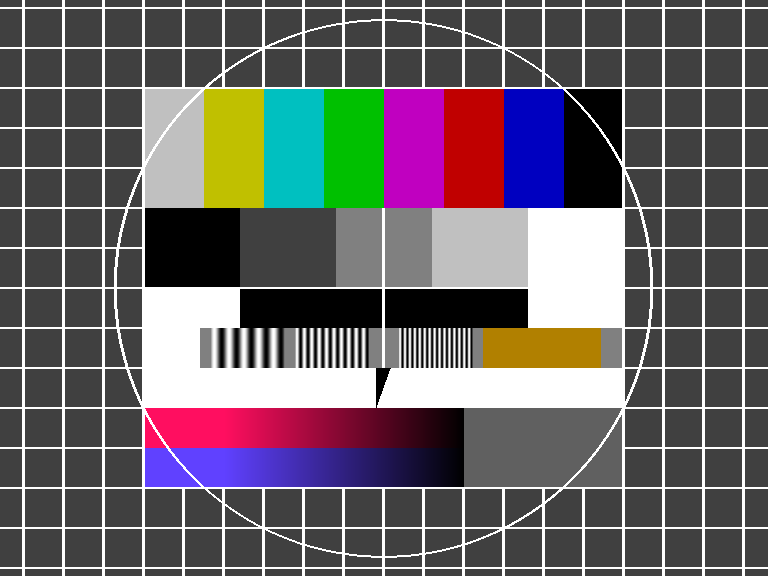
\includegraphics[width=0.3\textwidth]{images/testimage.png}
  \caption[Short figure caption]{Long figure caption displayed
  in the document.}
  \label{fig:figures:1}
\end{figure}
\end{filecontents*}

\IfElsePackageLoaded{graphicx}{%

\subsection{figure environment}
\label{sec:demo:figures:figure}

\PrintDemo{style=stacked}%

}{\DemoError{Package \package{graphicx} not loaded}}%

%% ------------------------------------------------------------
\begin{filecontents*}{\democodefile}
\begin{center}
  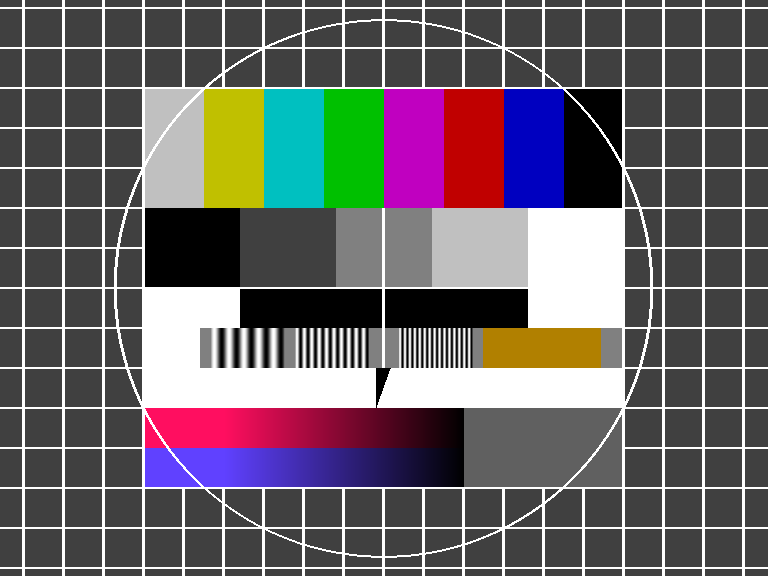
\includegraphics[width=0.3\textwidth]{images/testimage.png}
  \captionof{figure}{An example for a caption without a figure environment}
\end{center}
\end{filecontents*}

\IfElsePackageLoaded{graphicx}{%

\subsection{caption without figure environment using captionof (caption)}
\label{sec:demo:figures:captionof}
\ifcsdef{captionof}{%

\enlargethispage{5\baselineskip}
\PrintDemo{style=stacked}%
\clearpage

}{\DemoError{Command \cs{captionof} not available}}%
}{}%

%% ------------------------------------------------------------
\begin{filecontents*}{\democodefile}
\begin{center}
  \captionsetup{type=figure}
  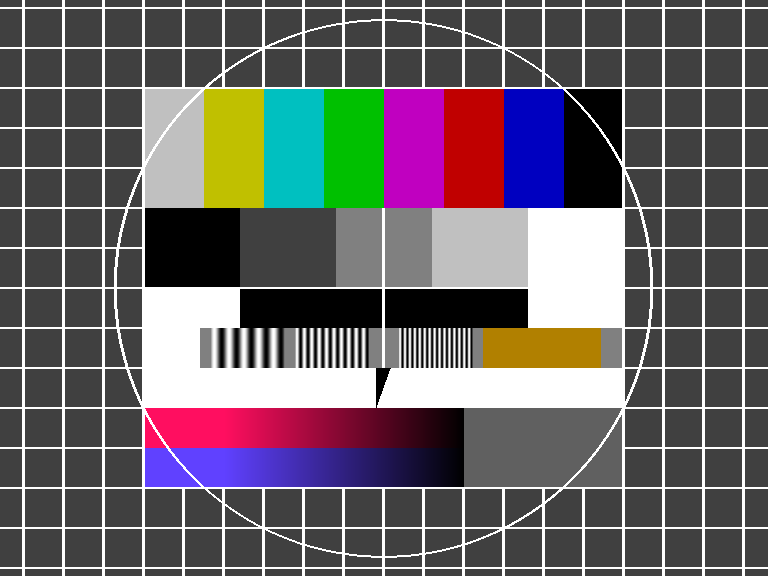
\includegraphics[width=0.3\textwidth]{images/testimage.png}
  \caption{Another example for a caption without a figure environment}
\end{center}
\end{filecontents*}

\IfElsePackageLoaded{graphicx}{%
\subsection{caption without figure environment using captionsetup (caption)}
\label{sec:demo:figures:captionsetup}

\ifcsdef{captionsetup}{%

\PrintDemo{style=stacked}%

}{\DemoError{Package \package{caption} not loaded}}%
}{}%

%% ------------------------------------------------------------
\begin{filecontents*}{\democodefile}
\begin{figure}[H]
  \IfDefined{RawFloats}{\RawFloats} % required if floatrow is loaded
  \begin{minipage}[b]{.5\linewidth}
    \centering
    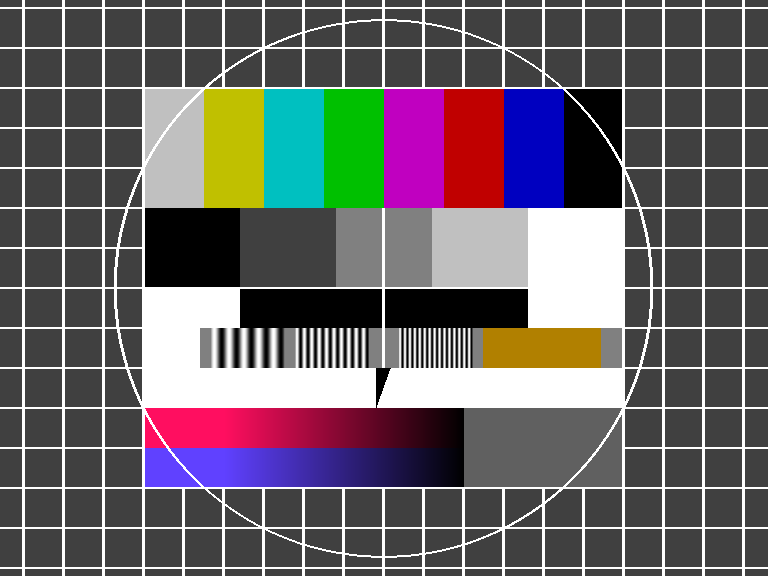
\includegraphics[width=0.5\linewidth]{images/testimage.png}
    \caption{A figure}
    \label{fig:figures:2}
  \end{minipage}%
  %\hspace{2em}
  \begin{minipage}[b]{.5\linewidth}
    \centering
    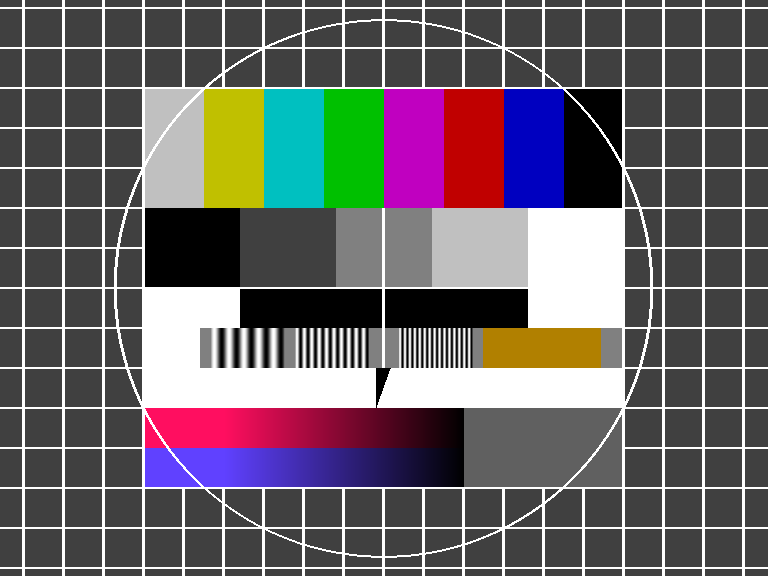
\includegraphics[width=0.5\linewidth]{images/testimage.png}
    \caption{Another figure}
    \label{fig:figures:3}
  \end{minipage}
\end{figure}
\end{filecontents*}

\IfElsePackageLoaded{graphicx}{%

\subsection{parallel figures with minipages}
\label{sec:demo:figures:minipage}

The \env{minipage} environment can be used to display figures in parallel.
However if the \package{floatrow} package is loaded the standard \latex{} behaviour must be restored using \cs{RawFloats} at the beginning of the figure.

\PrintDemo{style=stacked}%

}{\DemoError{Package \package{graphicx} not loaded}}%

%% ------------------------------------------------------------
\begin{filecontents*}{\democodefile}
\begin{figure}[H]
  \begin{minipage}[b]{.5\linewidth}
    \centering
    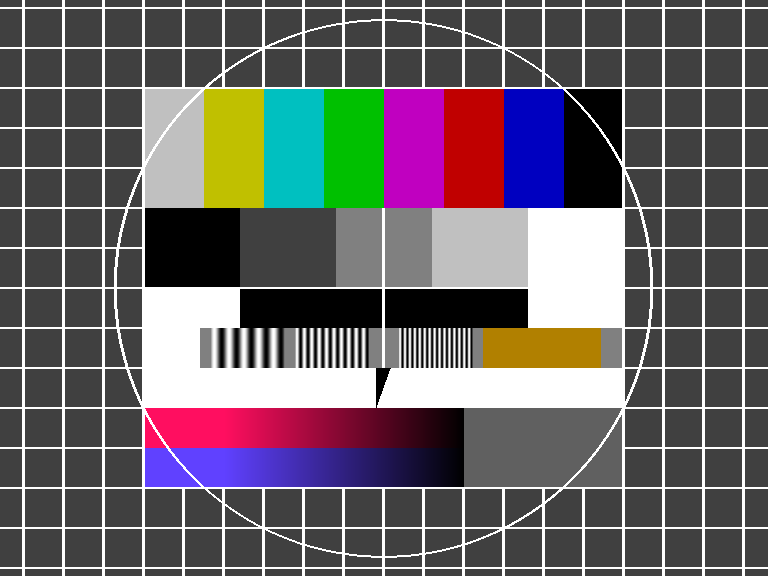
\includegraphics[width=0.5\linewidth]{images/testimage.png}
    \subcaption{A subfigure}\label{fig:1a}
  \end{minipage}%
  \begin{minipage}[b]{.5\linewidth}
    \centering
    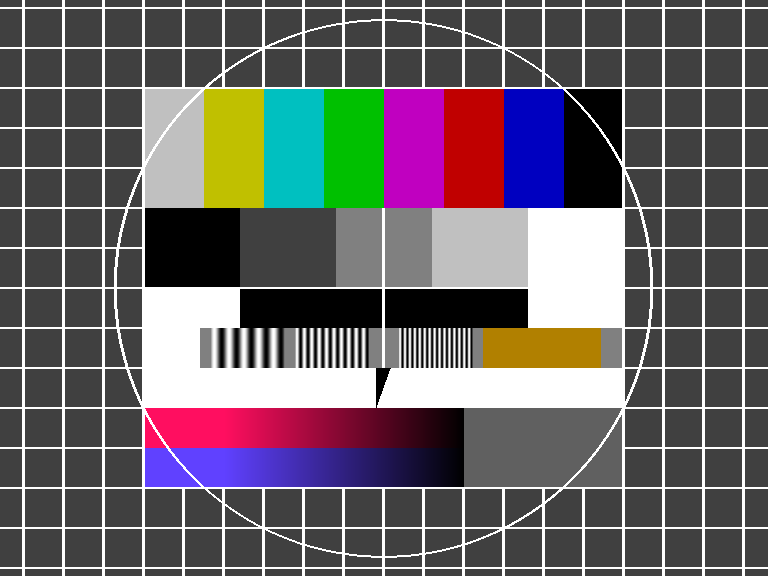
\includegraphics[width=0.5\linewidth]{images/testimage.png}
    \subcaption{Another subfigure}\label{fig:1b}
  \end{minipage}
  \caption{A figure}\label{fig:1}
\end{figure}
\end{filecontents*}

\IfElsePackageLoaded{graphicx}{%
\ifcsdef{subcaption}{%
%%
\subsection{subcaption in minipages (caption)}
\label{sec:demo:figures:subcaption}

The \cs{subcaption} command allows to define subfigure captions independent of the code used to display the pictures.

\PrintDemo{style=stacked}%

}{\DemoError{Package \package{subcaption} not loaded}}%
}{} % end if 

%% ------------------------------------------------------------
\begin{filecontents*}{\democodefile}
\begin{figure}[H]
  \begin{subfigure}[b]{.5\linewidth}
    \centering
    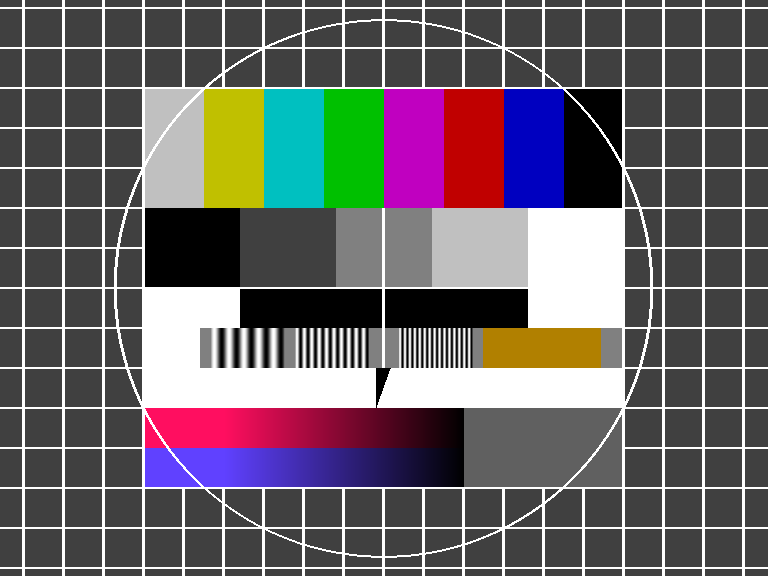
\includegraphics[width=0.5\linewidth]{images/testimage.png}
    \caption{A subfigure}\label{fig:2a}
  \end{subfigure}%
  \begin{subfigure}[b]{.5\linewidth}
    \centering
    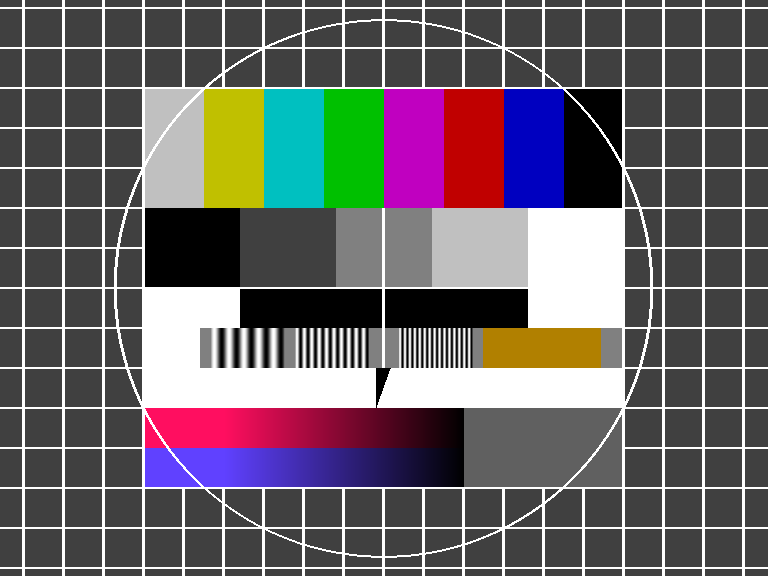
\includegraphics[width=0.5\linewidth]{images/testimage.png}
    \caption{Another subfigure}\label{fig:2b}
  \end{subfigure}
  \caption{A figure}\label{fig:2}
\end{figure}
\end{filecontents*}

\IfElsePackageLoaded{graphicx}{%
\ifcsdef{endsubfigure}{%

\subsection{subfigure environment (caption)}
\label{sec:demo:figures:subfigure}

The \env{subfigure} environment has a syntax equal to the normal figure environment, enhanced with the width and positioning arguments of a minipage environment.

\PrintDemo{style=stacked}%

}{\DemoError{Environment \env{subfigure} not available}}%
}{} % end if 


%% ------------------------------------------------------------
\begin{filecontents*}{\democodefile}
\begin{figure}[H]
  \centering
  \subfloat[first picture]{%
    \includegraphics[width=0.3\textwidth]%
    {images/testimage.png}}
    \hspace{0.1\textwidth}
  \subfloat[second picture]{%
    \includegraphics[width=0.3\textwidth]%
    {images/testimage.png}}
  \caption{An example for subfigures with subfloat}
\end{figure}
\end{filecontents*}

\IfElsePackageLoaded{graphicx}{%

\subsection{subcaption with subfloat command (subfig)}
\label{sec:demo:figures:subfloat}

\ifcsdef{subfloat}{%

\PrintDemo{style=stacked}%

}{\DemoError{Command \package{subfloat} not available}}%
}{}%

%% ------------------------------------------------------------
\begin{filecontents*}{\democodefile}
\begin{figure}[H]
\begin{floatrow}
\ffigbox[\FBwidth]
{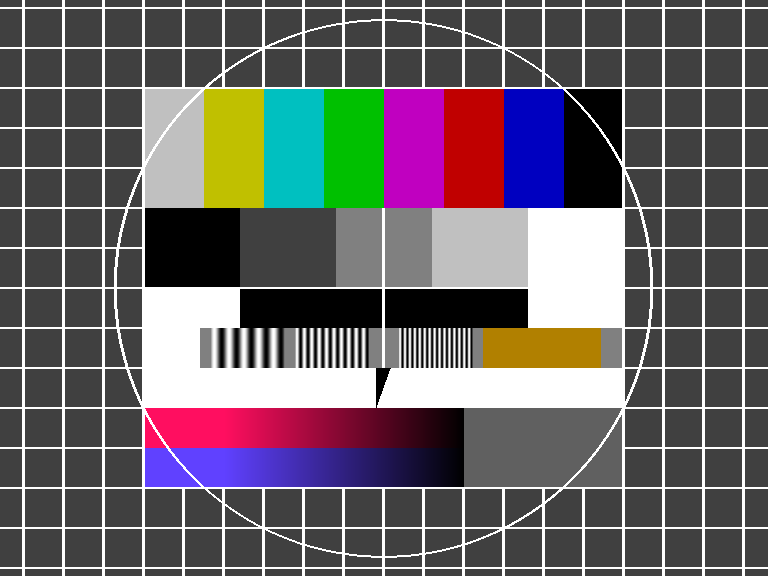
\includegraphics[width=0.3\textwidth]{images/testimage.png}}
{\caption{caption spanning the width of the picture}
 \label{fig:floatrow:example:3:a}}
%
\ffigbox[\Xhsize]
{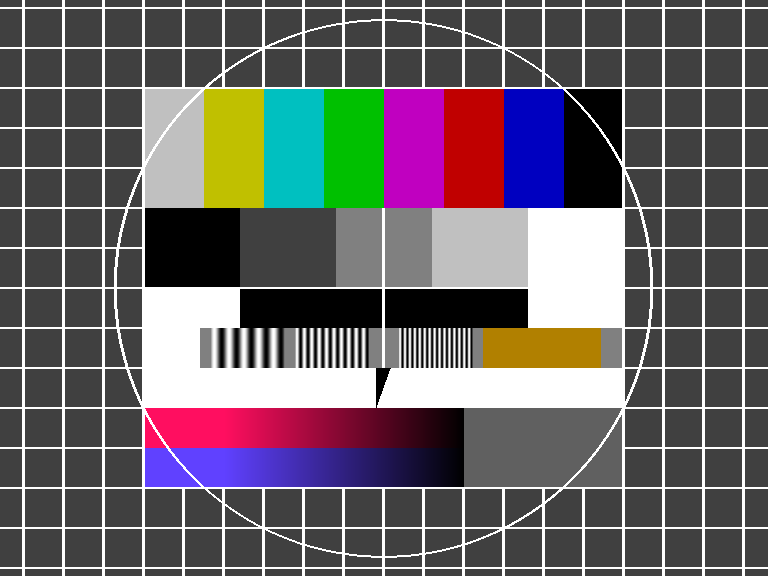
\includegraphics[width=0.3\textwidth]{images/testimage.png}}
{\caption{caption spanning the remaining width of the text width}
 \label{fig:floatrow:example:3:b}}
\end{floatrow}
\end{figure}
\end{filecontents*}

\IfElsePackageLoaded{graphicx}{%

\subsection{parallel figures (floatrow)}
\label{sec:demo:figures:floatrow:a}

\IfElsePackageLoaded{floatrow}{%

The \package{floatrow} package provides many ways to layout pictures and tables and any other floating content. Here is an example with the \cs{ffigbox} command inside the \env{floatrow} environment using the figure width for the first figure and the remaining width for the second figure.

\PrintDemo{style=stacked}%

}{\DemoError{Package \package{floatrow} not loaded}}%
}{}

%% ------------------------------------------------------------
\begin{filecontents*}{\democodefile}
\begin{figure}[H]
\begin{floatrow}
\floatbox{figure}[0.3\textwidth][\FBheight][t]
{\caption{first image positioned at the top}
 \label{fig:floatrow:example:4:a}}
{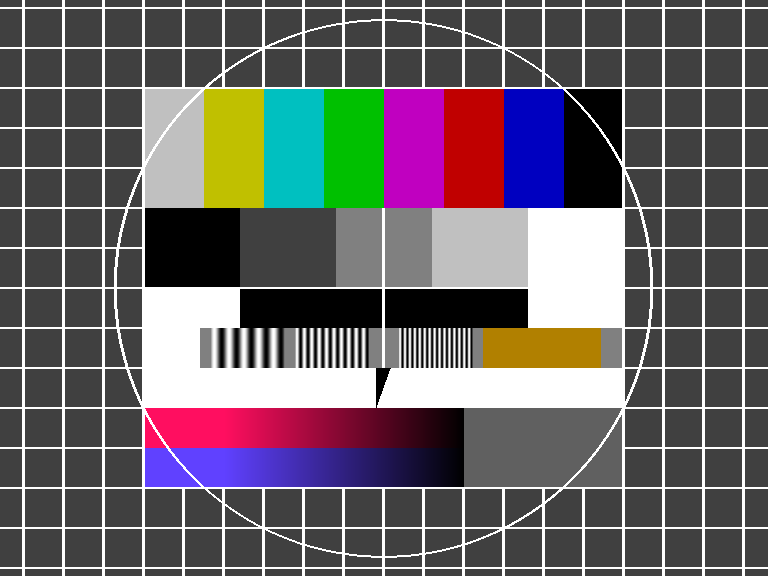
\includegraphics[width=0.25\textwidth]{images/testimage.png}}
%
\floatbox{figure}[0.3\textwidth][\FBheight][t]
{\caption{second image positioned at the top}
 \label{fig:floatrow:example:4:b}}
{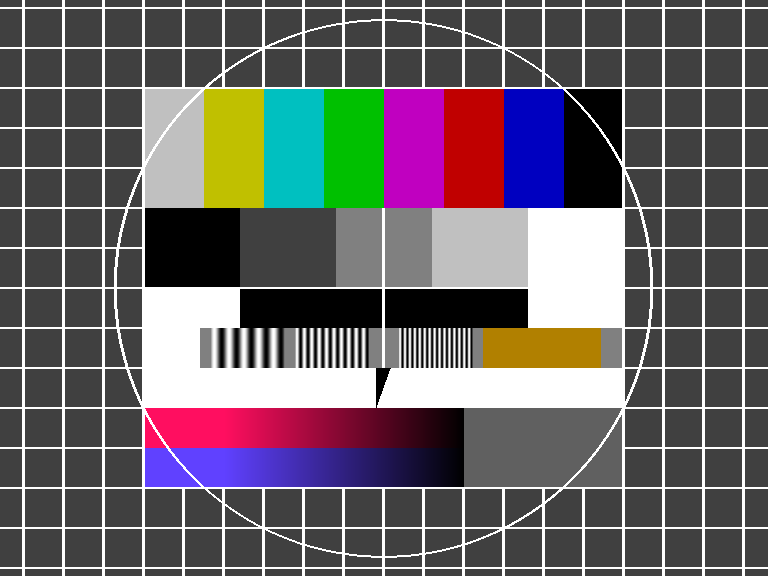
\includegraphics[width=0.15\textwidth]{images/testimage.png}}
%
\floatbox{figure}[0.3\textwidth][\FBheight][b]
{\caption{third image positioned at the bottom}
 \label{fig:floatrow:example:4:c}}
{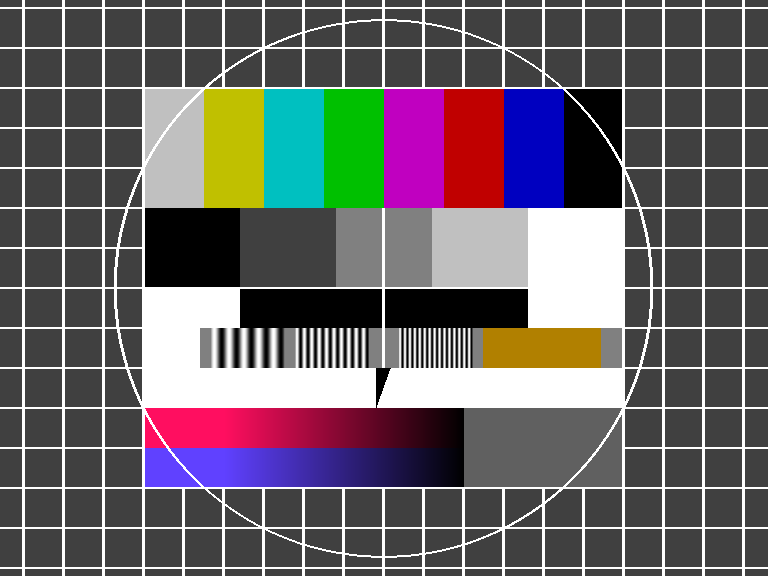
\includegraphics[width=0.15\textwidth]{images/testimage.png}}
\end{floatrow}
\end{figure}
\end{filecontents*}

\IfElsePackageLoaded{graphicx}{%
\subsection{parallel figures with vertical alignment (floatrow)}
\label{sec:demo:figures:floatrow:b}

\IfElsePackageLoaded{floatrow}{%

The general \cs{floatbox} command allows vertical alignment in the third optional parameter. Here [t]op and [b]ottom alignment is demonstrated.

\PrintDemo{style=stacked}%

}{\DemoError{Package \package{floatrow} not loaded}}%
}{}


%% ------------------------------------------------------------
\begin{filecontents*}{\democodefile}
\begin{figure}[H]
\ffigbox[\FBwidth]
{
\begin{subfloatrow}
  \ffigbox[1.5\FBwidth]
  {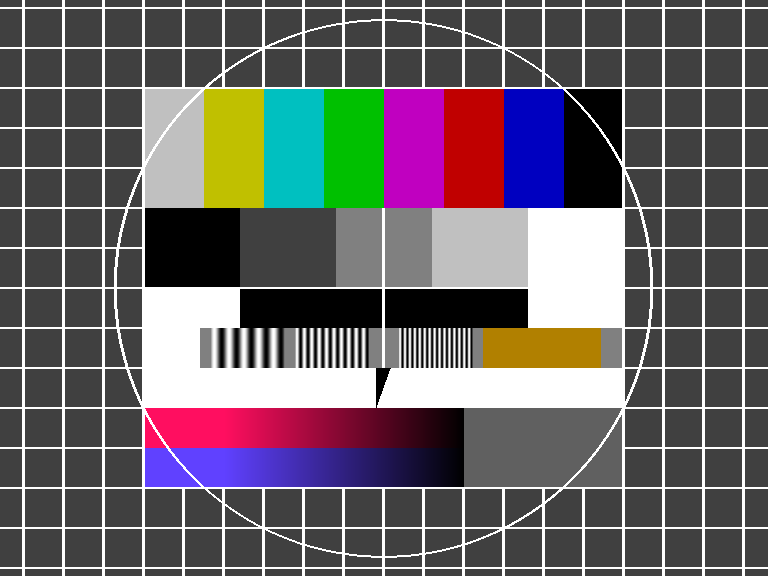
\includegraphics[width=0.2\textwidth]{images/testimage.png}}
  {\caption{first image}\label{fig:floatrow:example:5:a}}
%
  \ffigbox[1.5\FBwidth]
  {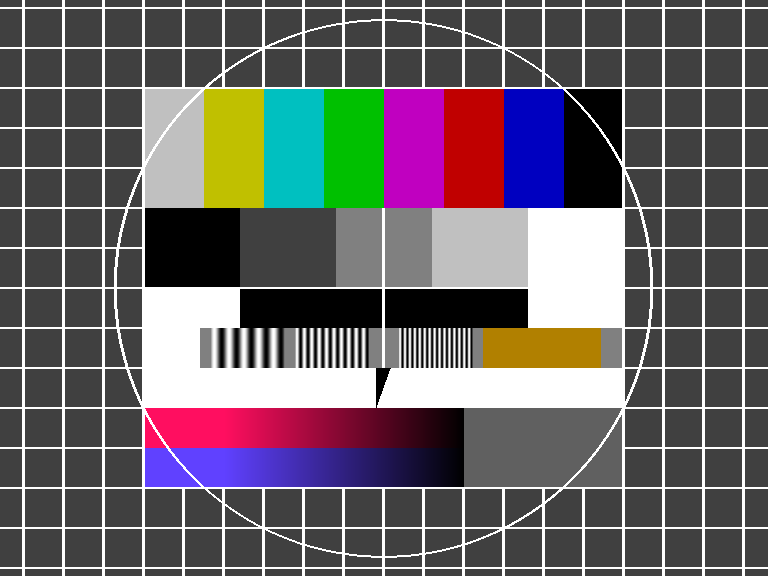
\includegraphics[width=0.2\textwidth]{images/testimage.png}}
  {\caption{second image}\label{fig:floatrow:example:5:b}}
\end{subfloatrow}
}
{\caption{subcaptions using subfloatrow environment}
 \label{fig:floatrow:example:5}}
\end{figure}
\end{filecontents*}

\IfElsePackageLoaded{graphicx}{%
\subsection{subfigures with subfloatrow environment (floatrow)}
\label{sec:demo:figures:floatrow:c}

\IfElsePackageLoaded{floatrow}{%

The figure placement and layout of \package{floatrow} can be changed to subfigures by using the \env{subfloatrow} environment.

\PrintDemo{style=stacked}%

}{\DemoError{Package \package{floatrow} not loaded}}%
}{}

%% ------------------------------------------------------------
\begin{filecontents*}{\democodefile}
\begin{figure}[H]
\floatbox[{\capbeside}]{figure}[\FBwidth]
{\caption[caption beside the figure]{caption beside the figure with some more 
text and a bit more text and a little more text to fill space}
 \label{fig:floatrow:example:6:a}}
{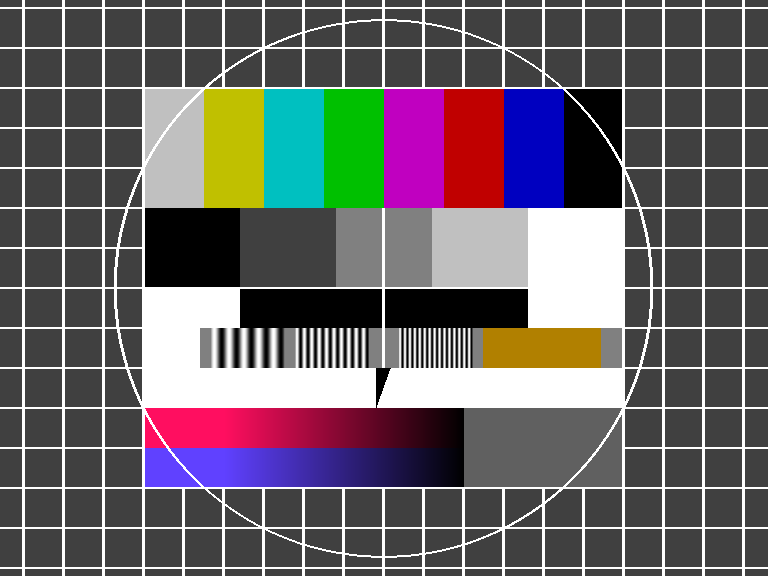
\includegraphics[width=0.3\textwidth]{images/testimage.png}}
\end{figure}
\end{filecontents*}

\IfElsePackageLoaded{graphicx}{%
\subsection{caption beside the figure (floatrow)}
\label{sec:demo:figures:floatrow:d}

\IfElsePackageLoaded{floatrow}{%

Using the first optional argument of \cs{floatbox} one can define a caption which is placed beside the figure with \cs{capbeside}.

\PrintDemo{style=stacked}%

}{\DemoError{Package \package{floatrow} not loaded}}%
}{}

%% ------------------------------------------------------------
\begin{filecontents*}{\democodefile}
\KOMAoptions{captions=bottombeside} % topbeside
\begin{figure}[H]
\IfDefined{RawFloats}{\RawFloats} % required if floatrow is loaded
\begin{captionbeside}%
  [Example of captionbeside]%
  {Example of captionbeside, with inside caption and with some more 
  text and a bit more text and a little more text to fill space.}%
  [i][0.9\textwidth][2em]
    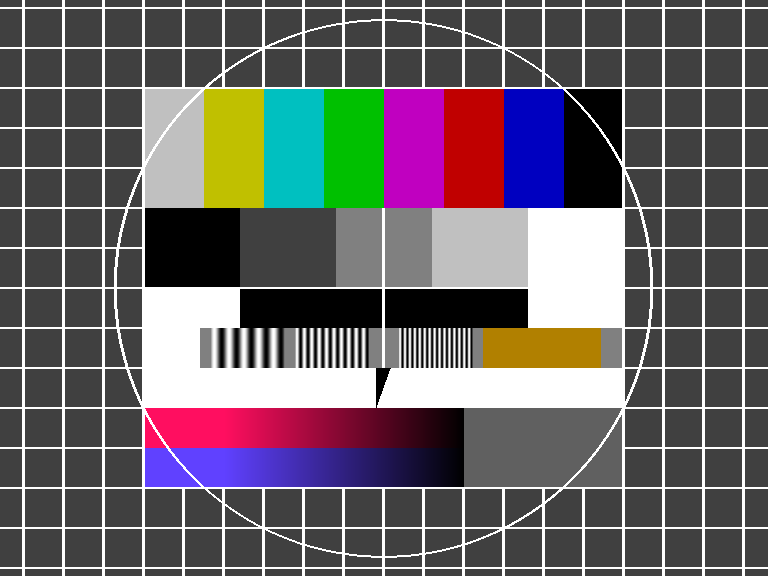
\includegraphics[width=0.3\textwidth]{images/testimage.png}
\end{captionbeside}
\label{fig:captionbeside:example}
\end{figure}
\end{filecontents*}

\IfElsePackageLoaded{graphicx}{%
\subsection{caption beside the figure with captionbeside (koma script)}
\label{sec:demo:figures:captionbeside}

\ifcsdef{captionbeside}{%

If the \package{floatrow} package is loaded the standard \latex{} behaviour must be restored using \cs{RawFloats} at the beginning of the figure.

\PrintDemo{style=stacked}%

}{\DemoError{Environment \env{captionbeside} not available}}%
}{}

%% ------------------------------------------------------------
\clearpage
\begin{filecontents*}{\democodefile}
\begin{wrapfigure}{r}{0.3\textwidth}
  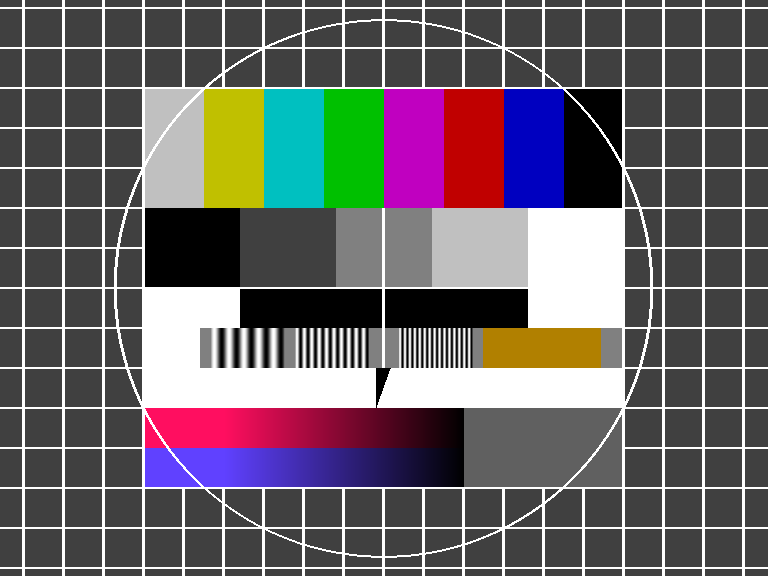
\includegraphics[width=0.8\linewidth]{images/testimage.png}
  \caption{A wrapfigure example}
   %\vspace{-2\baselineskip}
\end{wrapfigure}
...
\end{filecontents*}

\IfElsePackageLoaded{graphicx}{%
\subsection{figure inside the paragraph (wrapfigure)}
\label{sec:demo:figures:wrapfigure}

\ifcsdef{wrapfigure}{%

Non floating figure inside the paragraph. Note that this can cause
wrong placed free space in the text body. If so one must remove this by adding appropiate \cs{vspace} commands at the top and/or bottom of the figure.

\nopagebreak[4]
\vspace*{0.5em}\par\noindent
\printlatexcode%
\demoresultprefix
\begin{framed}%

\begin{wrapfigure}{r}{0.3\textwidth}
  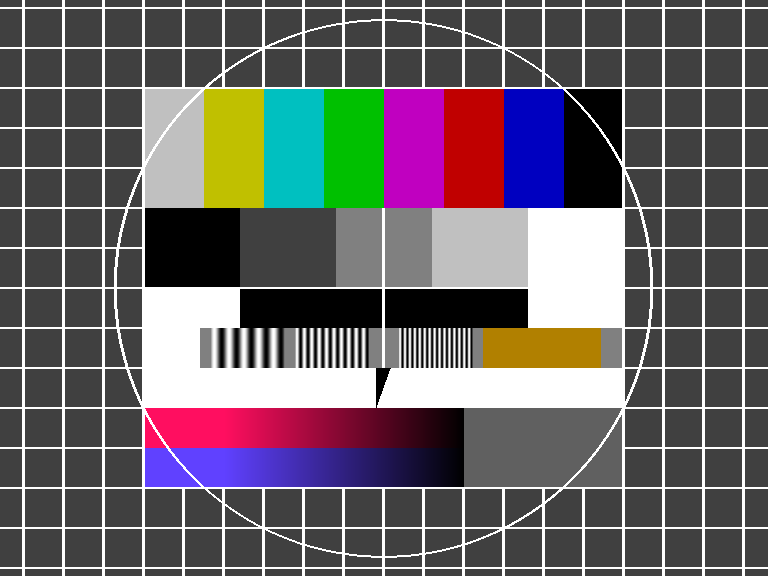
\includegraphics[width=0.8\linewidth]{images/testimage.png}
  \caption{A wrapfigure example}
   %\vspace{-2\baselineskip}
\end{wrapfigure}
Suspendisse vel felis. Ut lorem lorem, interdum
eu, tincidunt sit amet, laoreet vitae, arcu. Aenean faucibus pede eu
ante. Praesent enim elit, rutrum at, molestie non, nonummy vel,
nisl. Ut lectus eros, malesuada sit amet, fermentum eu, sodales
cursus, magna. Donec eu purus. Quisque vehicula, urna sed ultricies
auctor, pede lorem egestas dui, et convallis elit erat sed nulla.
Donec luctus. Curabitur et nunc. Aliquam dolor odio, commodo
pretium, ultricies non, pharetra in, velit. Integer arcu est,
nonummy in, fermentum faucibus, egestas vel, odio.
Suspendisse vel felis. Ut lorem lorem, interdum
eu, tincidunt sit amet, laoreet vitae, arcu. Aenean faucibus pede eu
ante. Praesent enim elit, rutrum at, molestie non, nonummy vel,
nisl. Ut lectus eros, malesuada sit amet, fermentum eu, sodales
cursus, magna. Donec eu purus. Quisque vehicula, urna sed ultricies
auctor, pede lorem egestas dui, et convallis elit erat sed nulla.
Donec luctus.

\end{framed}

}{\DemoError{Environment \env{wrapfigure} not available}}%
}{}%


%% ------------------------------------------------------------
\begin{filecontents*}{\democodefile}
\begin{wrapfloat}{figure}{r}{0.3\textwidth}
  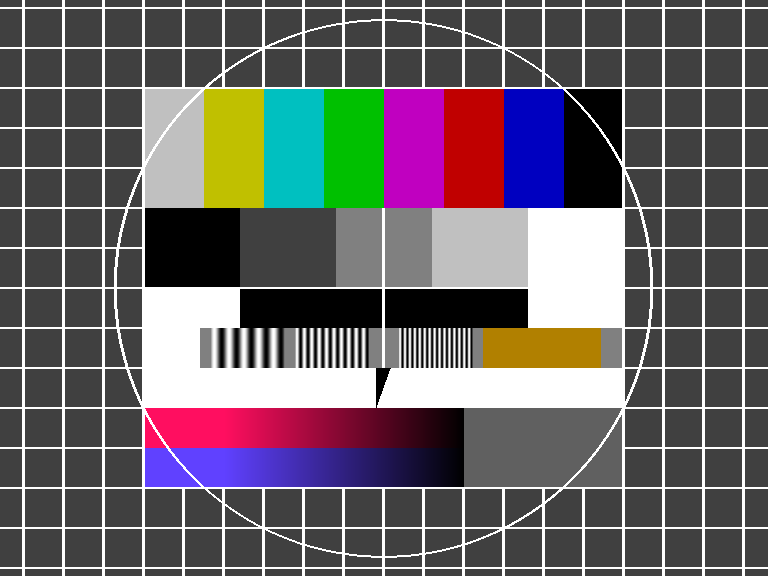
\includegraphics[width=0.8\linewidth]{images/testimage.png}
  \caption{A wrapfloat example}
   %\vspace{-2\baselineskip}
\end{wrapfloat}
...
\end{filecontents*}

\IfElsePackageLoaded{graphicx}{%
\subsection{floating figure (or table) inside the paragraph (wrapfigure)}
\label{sec:demo:figures:wrapfloat}

\ifcsdef{wrapfigure}{%

The \env{wrapfloat} environment in contrast to the \env{wrapfigure} environment is a floating environment and can be used for not only figures but any floating content.

\nopagebreak[4]
\vspace*{0.5em}\par\noindent
\printlatexcode%
\demoresultprefix
\begin{framed}%

\begin{wrapfloat}{figure}{r}{0.3\textwidth}
  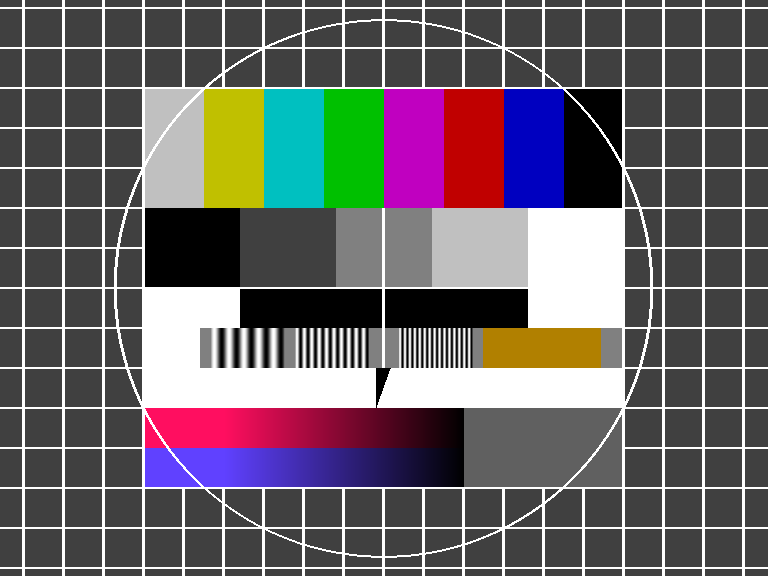
\includegraphics[width=0.8\linewidth]{images/testimage.png}
  \caption{A wrapfloat example}
   %\vspace{-2\baselineskip}
\end{wrapfloat}
Suspendisse vel felis. Ut lorem lorem, interdum
eu, tincidunt sit amet, laoreet vitae, arcu. Aenean faucibus pede eu
ante. Praesent enim elit, rutrum at, molestie non, nonummy vel,
nisl. Ut lectus eros, malesuada sit amet, fermentum eu, sodales
cursus, magna. Donec eu purus. Quisque vehicula, urna sed ultricies
auctor, pede lorem egestas dui, et convallis elit erat sed nulla.
Donec luctus. Curabitur et nunc. Aliquam dolor odio, commodo
pretium, ultricies non, pharetra in, velit. Integer arcu est,
nonummy in, fermentum faucibus, egestas vel, odio.
Suspendisse vel felis. Ut lorem lorem, interdum
eu, tincidunt sit amet, laoreet vitae, arcu. Aenean faucibus pede eu
ante. Praesent enim elit, rutrum at, molestie non, nonummy vel,
nisl. Ut lectus eros, malesuada sit amet, fermentum eu, sodales
cursus, magna. Donec eu purus. Quisque vehicula, urna sed ultricies
auctor, pede lorem egestas dui, et convallis elit erat sed nulla.
Donec luctus.

\end{framed}

}{\DemoError{Environment \env{wrapfloat} not available}}%
}{}


%% ------------------------------------------------------------
\begin{filecontents*}{\democodefile}
\begin{floatingfigure}[r]{0.3\textwidth}
   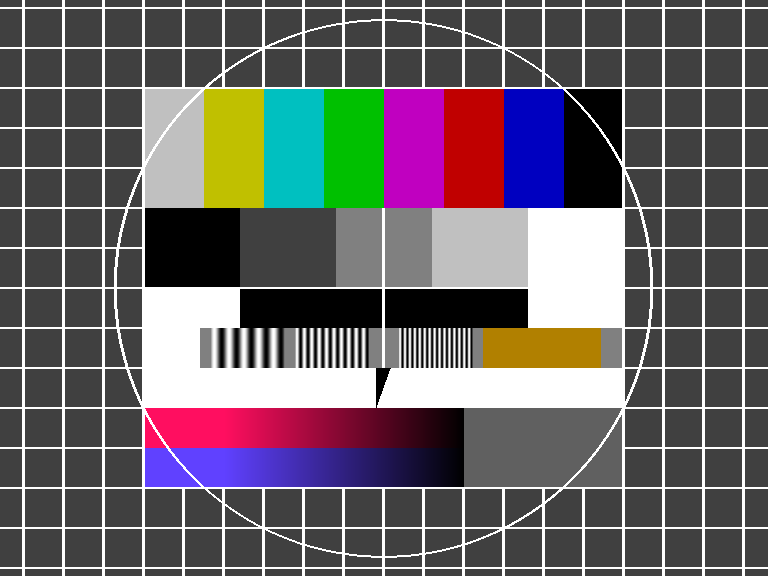
\includegraphics[width=0.25\textwidth]{images/testimage.png}
   \caption{A floatingfigure example}
\end{floatingfigure}
...
\end{filecontents*}

\IfElsePackageLoaded{graphicx}{%
\subsection{floating figure inside the paragraph (floatflt)}
\label{sec:demo:figures:floatflt}

\ifcsdef{endfloatingfigure}{%

The \env{floatingfigure} environment is a non-floating environment and can be used only for figures. It has however some layout problems compared to wrapfloat, for example the caption is larger than the image and the image size must be chosen smaller than the free space.

\nopagebreak[4]
\vspace*{0.5em}\par\noindent
\printlatexcode%
\demoresultprefix
\begin{framed}%

\begin{floatingfigure}[r]{0.3\textwidth}
   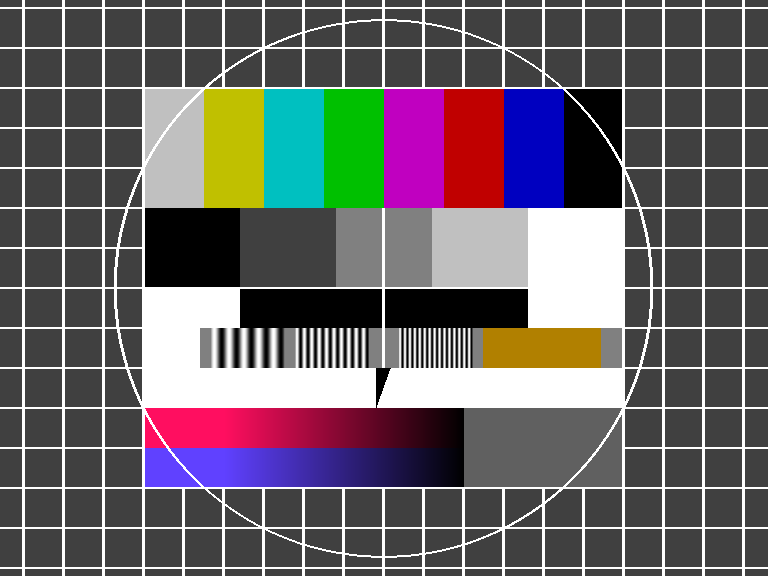
\includegraphics[width=0.25\textwidth]{images/testimage.png}
   \caption{A floatingfigure example}
\end{floatingfigure}
Suspendisse vel felis. Ut lorem lorem, interdum
eu, tincidunt sit amet, laoreet vitae, arcu. Aenean faucibus pede eu
ante. Praesent enim elit, rutrum at, molestie non, nonummy vel,
nisl. Ut lectus eros, malesuada sit amet, fermentum eu, sodales
cursus, magna. Donec eu purus. Quisque vehicula, urna sed ultricies
auctor, pede lorem egestas dui, et convallis elit erat sed nulla.
Donec luctus. Curabitur et nunc. Aliquam dolor odio, commodo
pretium, ultricies non, pharetra in, velit. Integer arcu est,
nonummy in, fermentum faucibus, egestas vel, odio.
Suspendisse vel felis. Ut lorem lorem, interdum
eu, tincidunt sit amet, laoreet vitae, arcu. Aenean faucibus pede eu
ante. Praesent enim elit, rutrum at, molestie non, nonummy vel,
nisl. Ut lectus eros, malesuada sit amet, fermentum eu, sodales
cursus, magna. Donec eu purus. Quisque vehicula, urna sed ultricies
auctor, pede lorem egestas dui, et convallis elit erat sed nulla.
Donec luctus.

\end{framed}

}{\DemoError{Environment \env{floatingfigure} not available}}%
}{}
%
%% ------------------------------------------------------------
\begin{filecontents*}{\democodefile}
\captionsetup{parboxrestore=default}

Pellentesque mollis nunc sed mauris tempor molestie. Aliquam adipiscing 
nisi eu metus. Proin viverra odio ac lorem consequat condimentum. 
Suspendisse bibendum tellus.

\begin{figure}[H]
\IfDefined{RawFloats}{\RawFloats} % required if floatrow is loaded
\begin{addmargin*}[0pt]{-0.6\marginwidth}%
\centering
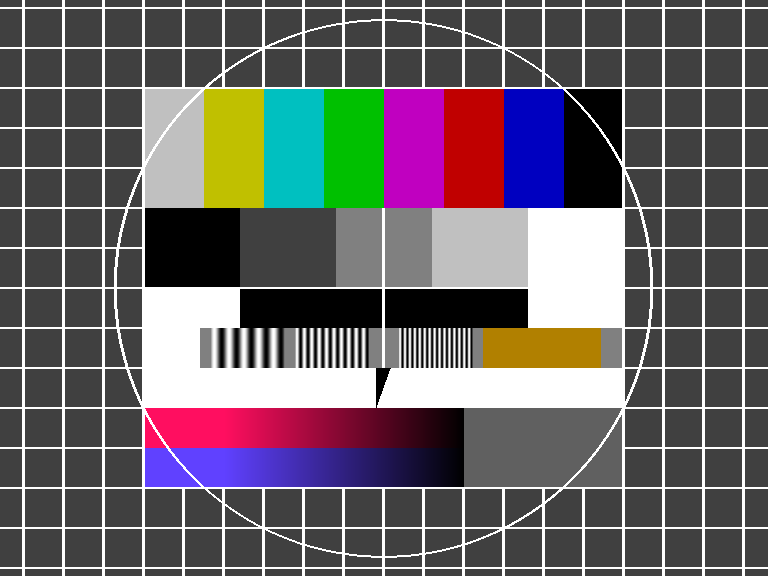
\includegraphics[width=0.22\linewidth]{images/testimage} \hfill
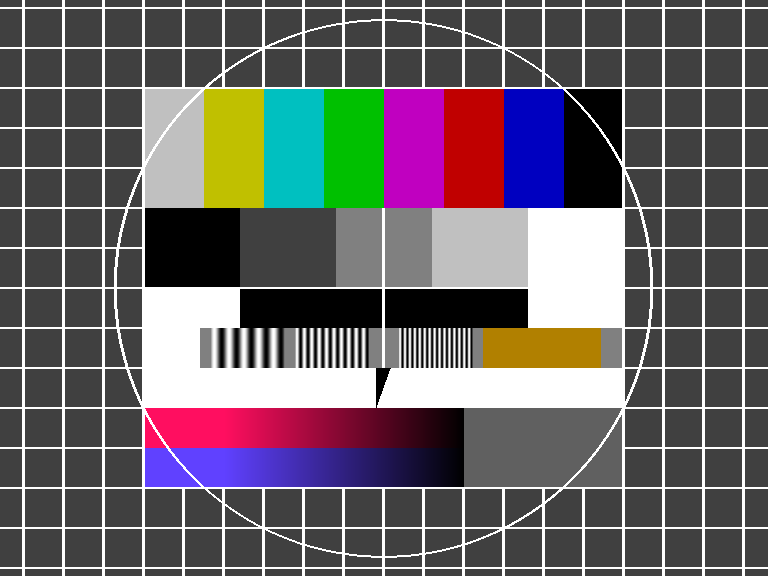
\includegraphics[width=0.22\linewidth]{images/testimage} \hfill
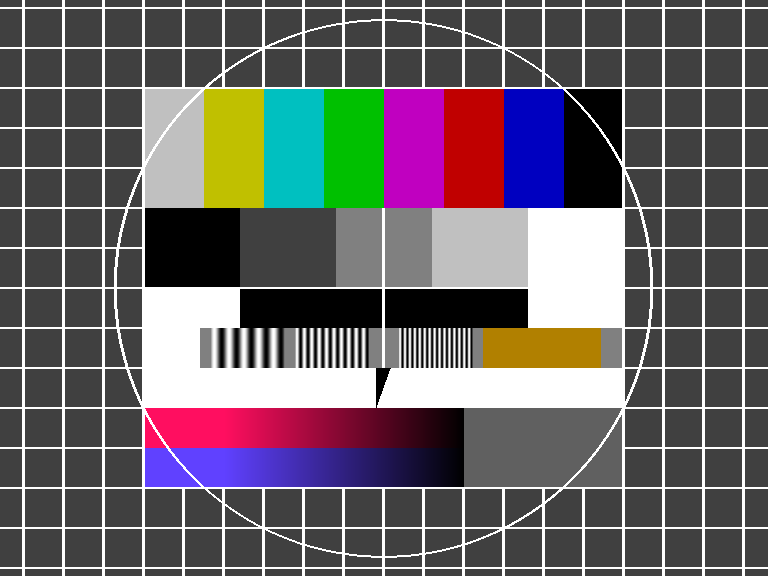
\includegraphics[width=0.22\linewidth]{images/testimage} \hfill
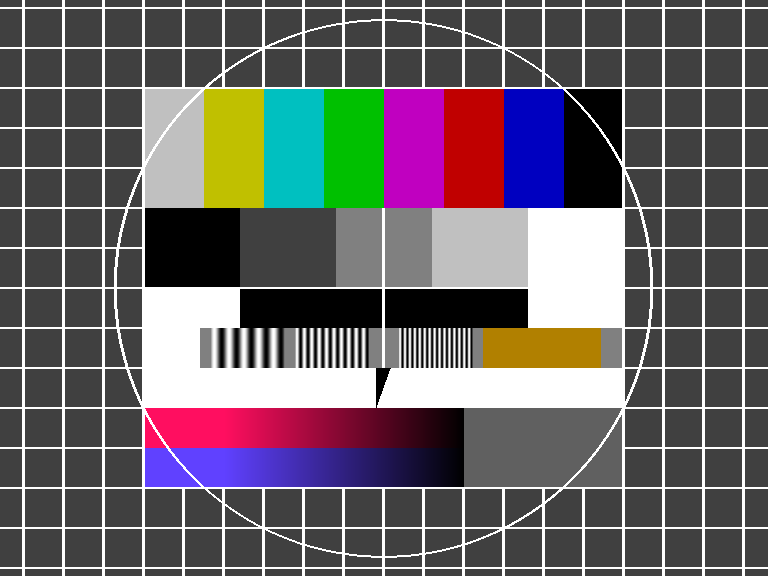
\includegraphics[width=0.22\linewidth]{images/testimage}
\caption[pictures extended into the margin]{pictures extended into the margin
-- Pellentesque mollis nunc sed mauris tempor molestie. Aliquam adipiscing
nisi eu metus. Proin viverra odio ac lorem consequat condimentum. Suspendisse
bibendum tellus. }
\label{fig:maincls.addmargin.default}
\end{addmargin*}
\end{figure}
%
Pellentesque mollis nunc sed mauris tempor molestie. Aliquam adipiscing 
nisi eu metus. Proin viverra odio ac lorem consequat condimentum. 
Suspendisse bibendum tellus.

\end{filecontents*}

\IfElsePackageLoaded{graphicx}{%
\subsection{Koma Script: addmargin (default)}
\label{sec:demo:figures:addmargin}

In this example the caption is as wide as the figure, which means that the caption spans into the margin.

\ifcsdef{addmargin}{%

\label{sec:figuresAddmargin}

\PrintDemo{style=lines}

}{\DemoError{Environment \env{addmargin} not available}}%
}{}%
%% ------------------------------------------------------------
\begin{filecontents*}{\democodefile}
\captionsetup{parboxrestore=full}

Pellentesque mollis nunc sed mauris tempor molestie. Aliquam adipiscing 
nisi eu metus. Proin viverra odio ac lorem consequat condimentum. 
Suspendisse bibendum tellus.

\begin{figure}[H]
\begin{addmargin*}[0pt]{-0.6\marginwidth}%
\centering
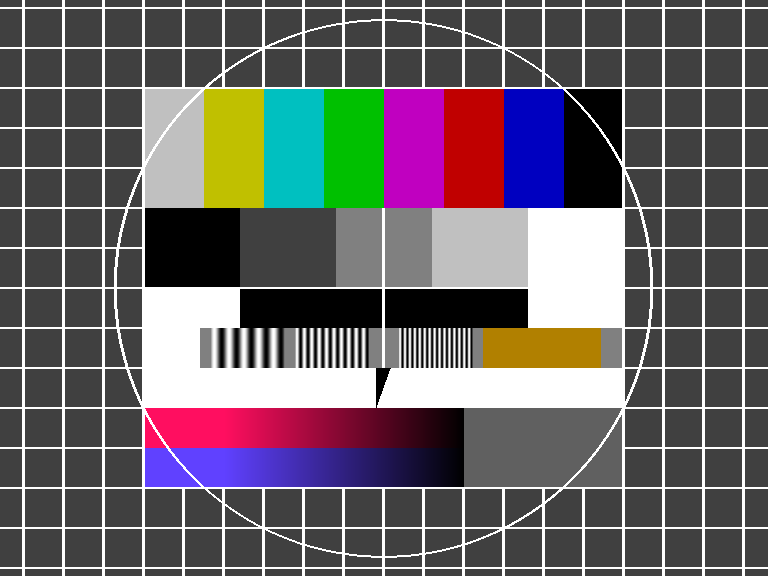
\includegraphics[width=0.22\linewidth]{images/testimage} \hfill
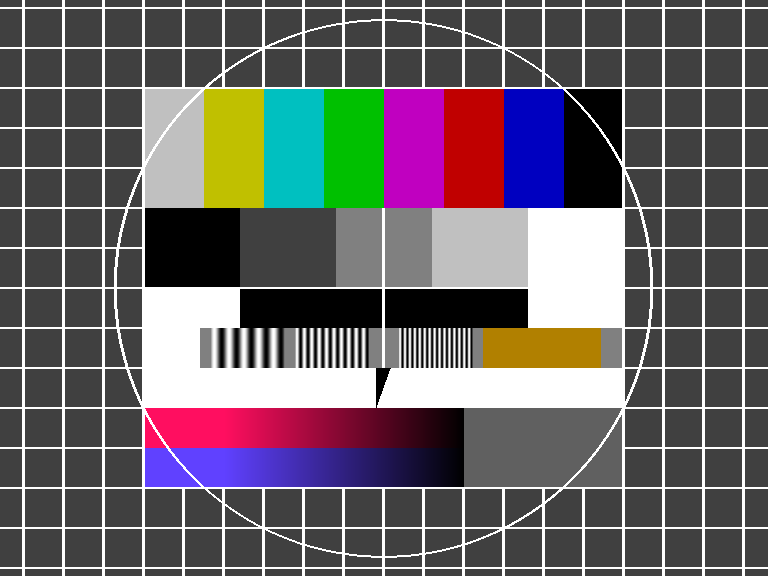
\includegraphics[width=0.22\linewidth]{images/testimage} \hfill
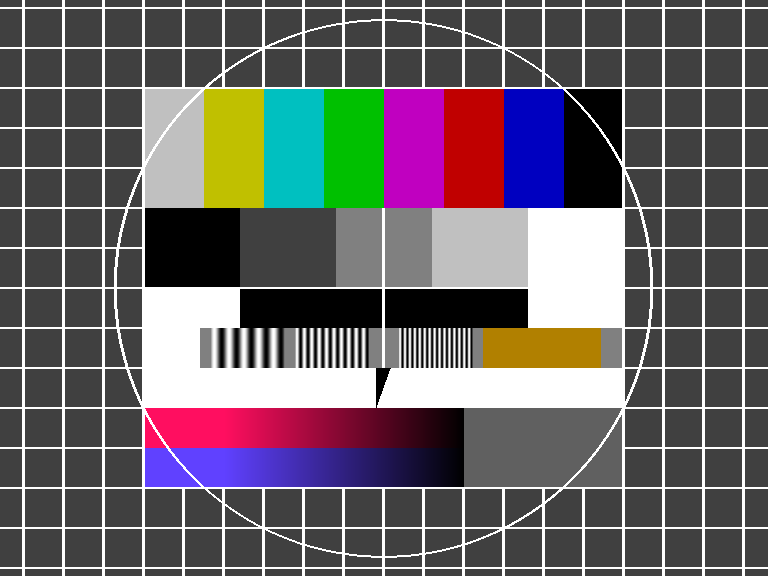
\includegraphics[width=0.22\linewidth]{images/testimage} \hfill
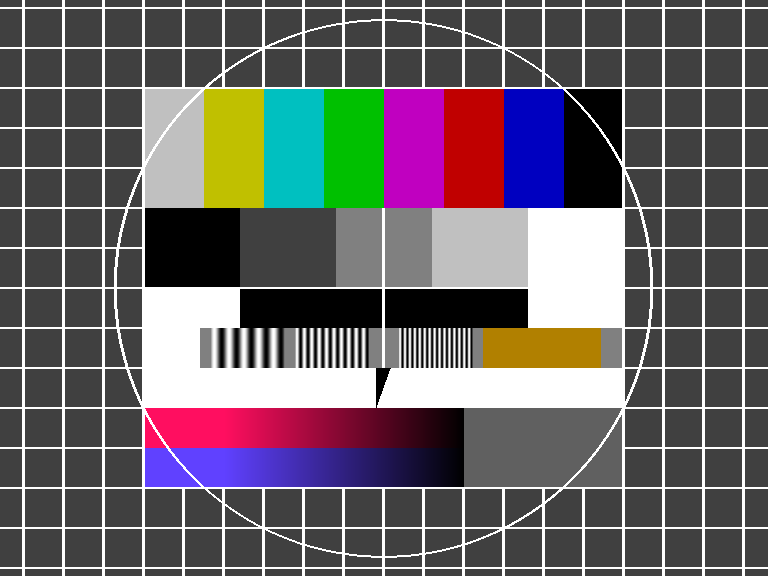
\includegraphics[width=0.22\linewidth]{images/testimage}
\caption[pictures extended into the margin]{pictures extended into the margin -- Pellentesque mollis nunc sed mauris tempor molestie. Aliquam adipiscing nisi eu metus. Proin viverra odio ac lorem consequat condimentum. Suspendisse bibendum tellus. }
\label{fig:maincls.addmargin.full}
\end{addmargin*}
\end{figure}
%
Pellentesque mollis nunc sed mauris tempor molestie. Aliquam adipiscing 
nisi eu metus. Proin viverra odio ac lorem consequat condimentum. 
Suspendisse bibendum tellus.
\end{filecontents*}

\IfElsePackageLoaded{graphicx}{%
\subsection{Koma Script: addmargin (with parboxrestore)}
\label{sec:demo:figures:addmargin:b}

Here the caption is only as wide as the textwidth, which is corrected using
the code \texttt{\bs{}captionsetup\{parboxrestore=full\}}.

\IfMultDefined{addmargin,captionsetup}{%

\PrintDemo{style=lines}%

}{\DemoError{Environment \env{addmargin} not available}}%
}{}%
%% ------------------------------------------------------------
\begin{filecontents*}{\democodefile}
Pellentesque mollis nunc sed mauris tempor molestie. Aliquam adipiscing nisi
eu metus. Proin viverra odio ac lorem consequat condimentum. Suspendisse
bibendum tellus. Duis non diam. Aliquam sodales sapien in mauris. Sed euismod
adipiscing lorem. Pellentesque nulla augue, nonummy vel, tincidunt at, blandit 

\begin{figure}[H]
\IfDefined{RawFloats}{\RawFloats} % required if floatrow is loaded
\begin{margincap}
  \centering
  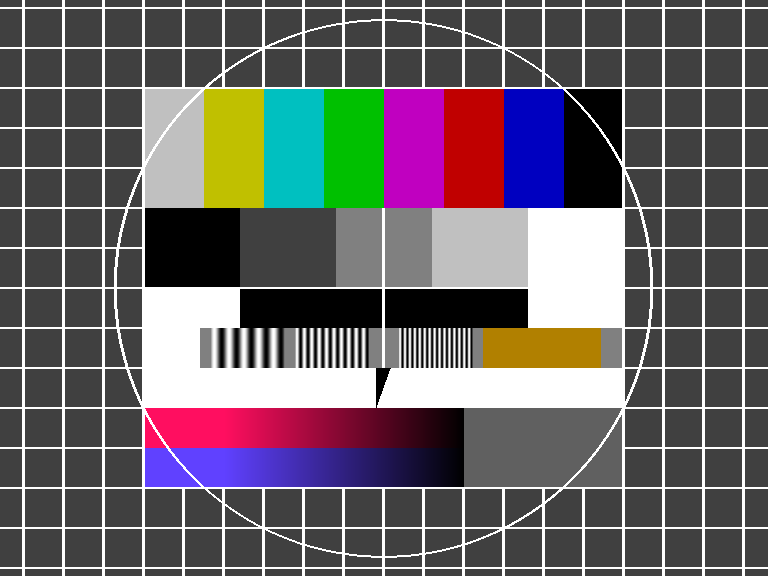
\includegraphics[width=0.4\textwidth]{images/testimage}
  \caption[short caption text]{long caption text with some more 
   text and a bit more text and a little more text to fill space.}
  \label{fig:picmargincap}
\end{margincap}
\end{figure}

Pellentesque mollis nunc sed mauris tempor molestie. Aliquam adipiscing nisi
eu metus. Proin viverra odio ac lorem consequat condimentum. Suspendisse
bibendum tellus. Duis non diam. Aliquam sodales sapien in mauris. Sed euismod
adipiscing lorem. Pellentesque nulla augue, nonummy vel, tincidunt at, blandit 
\end{filecontents*}

\IfElsePackageLoaded{graphicx}{%
\subsection{caption inside the margin (mcaption)}
\label{sec:demo:figures:mcaption}

\ifcsdef{margincap}{%

\nopagebreak[4]
\vspace*{0.5em}\par\noindent
\printlatexcode%
\printlatexresultlines

}{\DemoError{Package \package{mcaption} not loaded}}%
}{}%
% ------------------------------------------------------------

%% ------------------------------------------------------------
\subsection{document sizes}
\label{sec:demo:figures:doctextwidth}

\ifcslength{doctextwidth}{%

This template defines the commands \cs{doctextwidth} and \cs{doctextheight} which maintain their size even if the surrounding \cs{textwidth} changes. 
\vspace{0.5\baselineskip} \\ \noindent
These sizes can be used in figures to specify the width in fixed paper depended sizes.
\vspace{0.5\baselineskip} \\ \noindent
\fbox{\begin{minipage}{0.8\textwidth}
  0.8\bs{}textwidth \\[1em]
  \fbox{\begin{minipage}{0.38\doctextwidth}
    0.38\bs{}doctextwidth 
  \end{minipage}}
  \fbox{\begin{minipage}{0.38\doctextwidth}
    0.38\bs{}doctextwidth 
  \end{minipage}} \\
  \fbox{\begin{minipage}{0.38\textwidth}
    0.38\bs{}textwidth 
  \end{minipage}}
  \fbox{\begin{minipage}{0.38\textwidth}
    0.38\bs{}textwidth 
  \end{minipage}}
\end{minipage}}

}{\DemoError{Length \env{doctextwidth} not defined}}%

\EndCodeSection{DemoFigures}
%% ============================================================
\BeginCodeSection{DemoTables}
\clearpage
\section{Tables}
\label{sec:demo:tables}
%
This section about tables is organized as follows:
\begin{itemize}
\item In section~\ref{sec:tableStylesIntro} different styles to create a table are shown: 
  \begin{itemize}
  \item using booktabs line commands (\ref{sec:tableStyleBooktabs1} and
        \ref{sec:tableStyleBooktabs2}),
  \item with custom commands for the style and the colors
        (\ref{sec:tableStyleCustom}), 
  \item and with the package \package{tablestyles}
        (\ref{sec:tableStylePackage}).
  \end{itemize}
%
\item Section \ref{sec:tableColumnTypes} is about
      the alignment of columns in a table, the usage of column specifiers and the alignment of numbers using \package{siunitx}.
%
\item In section \ref{sec:tableMultiColumnRow} the usage of 
      \cs{multicolumn} and \cs{multirow} commands is shown.
%
\item Section \ref{sec:tableitemlists} shows how to correct the indentation
      for itemize lists.
%
\item Section \ref{sec:tablecolors} demonstrates the coloring of rows.
%
\item Section \ref{sec:tableTabuPackage} 
      introduces the creation of tables with the \package{tabu} package.
%
\item How to create and present very large tables is introduced in section~\ref{sec:TableLarge}.
\end{itemize}

%% ------------------------------------------------------------
\subsection{table styles}
\label{sec:tableStylesIntro}

There a many ways to design a table in terms of its lines (grid), sizes, fonts and colors. Most of these can be regarded as personal taste. However the simplest on, the grid design, is regarded as a style which should be avoided by any means, since it makes it difficult for the eye to read the table.
Here some of the most common approaches to style a table are presented.

%% ------------------------------------------------------------
\begin{filecontents*}{\democodefile}
\begin{table}[H]
% style
\small\sffamily\renewcommand{\arraystretch}{1.4}
% caption
\captionabove{table in booktabs style}
\begin{tabular}{lll}
\toprule
  header  & header  & header \\
\midrule
  content & content & content \\
  content & content & content \\
  content & content & content \\
\bottomrule
\end{tabular}
\end{table}
\end{filecontents*}

\subsubsection{Booktabs package}
\label{sec:tableStyleBooktabs1}

\IfMultDefined{toprule,captionabove}{%

\PrintDemo{style=stacked}%

}{\DemoError{Package \package{booktabs} or \package{caption} not loaded}}%

\begin{filecontents*}{\democodefile}
\small\sffamily\renewcommand{\arraystretch}{1.4}
\end{filecontents*}

\ifcsdef{toprule}{%
\noindent
Note that here the style of the table was further changed by the commands:
\lstinputlisting[style=demostyle,nolol=true]{\democodefile}%

}{}%

%% ------------------------------------------------------------
\begin{filecontents*}{\democodefile}
\begin{table}[H]
\small\sffamily\renewcommand{\arraystretch}{1.4}
\begin{tabular}{lll}
\toprule
  header  & header  & header \\ \cmidrule(r){1-1}
                                \cmidrule(lr){2-2}
                                \cmidrule(l){3-3}
  content & content & content \\
  content & content & content \\
  content & content & content \\
\bottomrule
\end{tabular}
\end{table}
\end{filecontents*}

\subsubsection{Cmidrule (booktabs)}
\label{sec:tableStyleBooktabs2}

\ifcsdef{cmidrule}{%

\PrintDemo{style=stacked}%

}{\DemoError{Package \package{booktabs} not loaded}}%



%% ------------------------------------------------------------
\begin{filecontents*}{\democodefile}
\begin{table}[H]
% style
\small\sffamily\centering\renewcommand{\arraystretch}{1.4}
% caption
\captionabove{table with style changes and zebra colored rows}
%tabular
\rowcolors{1}{tablebodycolor}{tablerowcolor}
\begin{tabular}{ccc}
\hline
\rowcolor{tableheadcolor}
  \bfseries header  & 
  \bfseries header  & 
  \bfseries header  \\
\hline
  content & content & content \\
  content & content & content \\
  content & content & content \\
\hline
\end{tabular}
\end{table}
\end{filecontents*}

\subsubsection{Custom style with alternating row colors}
\label{sec:tableStyleCustom}


\IfMultDefined{captionabove,rowcolors}{%
\IfColorsDefined{tablebodycolor,tablerowcolor,tableheadcolor}{%

Here a custom style is applied
\begin{itemize}
\item \cs{small} \hfill tables are more compact.
\item \cs{renewcommand}\{\cs{arraystretch}\}\{1.4\} \hfill better readibility of rows.
\item \cs{sffamily} \hfill tables are better distinguished from the main text.
\end{itemize}

\PrintDemo{style=stacked}%

}{\DemoError{Colors not defined}}%
}{\DemoError{Package \package{xcolor} or \package{caption} not loaded}}%


%% ------------------------------------------------------------
\begin{filecontents*}{\democodefile}
\begin{table}[H]
%
\tablestyle[sansbold]
%
\captionabove{table with bold header font using the styles by this package}
\begin{tabular}{*{2}{p{0.45\textwidth}}}
\theadstart
    \thead header &
    \thead header \\
\tbody
%
 content  & content \\
 content  & content \\
 content  & content \\
 content  & content \\
 content  & content \\
%
\tsubheadstart
 \tsubhead subhead &
 \tsubhead subhead \\
%
 content  & content \\
 content  & content \\
\tend
\end{tabular}
\end{table} 
\end{filecontents*}

\subsubsection{Tablestyles package}
\label{sec:tableStylePackage}

This package unifies the application of a style to a table. The following styles are predefined: \texttt{default}, \texttt{roman} (serif instead of sans fonts), \texttt{sansbold} (bold header), \texttt{sansboldbw} (white text on black background)

\IfMultDefined{captionabove,rowcolors,theadstart}{%

\PrintDemo{style=stacked}%

One should note, that these commands do not work together with the package \package{tabu}, since in that package most row color command do not work as expected or need to be replaced by color commands from the tabu package, see section~\ref{sec:tabletabucolor}.

}{\DemoError{Packages \package{xcolor}, \package{caption} or \package{tablestyles} not loaded}}%



%% ------------------------------------------------------------
\subsection{Column types and column specifiers}
\label{sec:tableColumnTypes}
%% ------------------------------------------------------------

\begin{filecontents*}{\democodefile}
\begin{tabular}{lcr} 
left  &  center  &  right  \\  % or \tabularnewline
A     &  B       &  C  \\
\end{tabular}
\end{filecontents*}

\subsubsection{Simple table (only alignment)}
\label{sec:simpletable}
\PrintDemo{style=stacked}%

%% ------------------------------------------------------------
\subsubsection{Column types: p}

\begin{filecontents*}{\democodefile}
\begin{center}
% Style changes
\small\renewcommand{\arraystretch}{1.4}
% tabular
\begin{tabular}{|l|p{0.1\linewidth}|p{0.2\linewidth}|p{0.4\linewidth}|}
\hline
header l & header p & header p & header p \\ \hline
%
left  &
text which is considerably longer than the width of the column & 
text which is considerably longer than the width of the column & 
text which is considerably longer than the width of the column 
\newline with a line break included \\ \hline
\end{tabular}
\end{center}
\end{filecontents*}

\IfColumntypeDefined{p}{%

p-columns have a fixed width and align the text as justified.

\PrintDemo{style=stacked}%

\noindent
Note, that such a grid should not be applied to a table.
It is here only to demonstrate the size of the columns.

}{\DemoError{Column type \env{p} not defined}}%

%% ------------------------------------------------------------
\subsubsection{Column types: p, m, b}

\begin{filecontents*}{\democodefile}
\begin{center}
% Style changes
\small\renewcommand{\arraystretch}{1.4}
% tabular
\begin{tabular}{|p{0.3\linewidth}|m{0.3\linewidth}|b{0.3\linewidth}|}
\hline
\centering header p &
\centering header m &   
\centering header b \tabularnewline
\hline
text which is considerably longer than the width of the column  & 
text which is considerably longer than the width of the column  & 
text which is considerably longer than the width of the column 
\\
\hline
\end{tabular}
\end{center}
\end{filecontents*}

\IfColumntypeDefined{p}{%

The p,b and m columns all behave the same expect for their vertical alignment:
\begin{itemize}
\item  p means normal cells, they aligned at the top line
\item  b means alignment at the bottom, so the baseline is at the bottom line
\item  m means alignment in the vertical center, i.e. the baseline is in the center.
\end{itemize}
Therefore b-columns are on top of p-columns because their baselines are aligned.

\PrintDemo{style=stacked}%

\noindent
Note, that such a grid should not be applied to a table.
It is here only to demonstrate the alignment.

}{\DemoError{Column types \env{p,m,b} not defined}}%

%% ------------------------------------------------------------
\subsubsection{Column types: X (tabularx)}

\begin{filecontents*}{\democodefile}
\begin{center}
% Style changes
\small\renewcommand{\arraystretch}{1.4}
% tabular
\small
\begin{tabularx}{0.9\textwidth}{llXX}
\hline
l & l & X & X \\\hline
%
left column & left column & 
text which is considerably longer than the width of the column & 
text which is considerably longer than the width of the column \\
\hline
\end{tabularx}
\end{center}
\end{filecontents*}

\IfColumntypeDefined{X}{%
\ifcsdef{tabularx}{

The package \package{tabularx} defines a new tabular environment, which requires the total width of the tabular as a mandatory argument. The new X-columns take the remaining space to fill the tabular. 
Each column is aligned as justified.

\PrintDemo{style=stacked}%

\noindent
Note, that such a grid should not be applied to a table.
It is here only to demonstrate the size of the columns.

}{\DemoError{Package \package{tabularx} not loaded}}%
}{\DemoError{Column types \env{X} not defined}}%

%% ------------------------------------------------------------
\subsubsection{Custom column types: L, C, R}
\label{sec:tablecolumnsLCR}

\begin{filecontents*}{\democodefile}
\begin{center}
% Style changes
\small\renewcommand{\arraystretch}{1.4}
% tabular
\small
\begin{tabular}{|L{0.3\linewidth}|C{0.3\linewidth}|R{0.3\linewidth}|}
\hline
fixed width (L: left)   & 
fixed width (C: center) &
fixed width (R: right)  \\ \hline
%
text which is considerably longer than the width of the column & 
text which is considerably longer than the width of the column & 
text which is considerably longer than the width of the column \\
\hline
\end{tabular}
\end{center}
\end{filecontents*}

\IfColumntypesDefined{L,C,R}{%

The predefined custom column types L, C and R all have a fixed width (they are based on the p-columns) but are aligned as left (L), centered (C) and right (R). All columns include hyphenation.

\PrintDemo{style=stacked}%

\noindent
Note, that such a grid should not be applied to a table.
It is here only to demonstrate the size and alignment of the columns.

}{\DemoError{Column types \env{L,C,R} not defined}}%

%% ------------------------------------------------------------
\subsubsection{Custom column types: W, Y, Z}
\label{sec:tablecolumnsWYZ}

\begin{filecontents*}{\democodefile}
\begin{center}
% Style changes
\small\renewcommand{\arraystretch}{1.4}
% tabular
\small
\begin{tabularx}{\textwidth}{|W|Z|Y|}
\hline
variable (W: left)   & 
variable (Z: center) &
variable (Y: right)  \\ \hline
%
text which is considerably longer than the width of the column & 
text which is considerably longer than the width of the column & 
text which is considerably longer than the width of the column \\
\hline
\end{tabularx}
\end{center}
\end{filecontents*}

\ifcsdef{tabularx}{
\IfColumntypesDefined{W,Y,Z}{%

The predefined custom column types W, Y and Z all have a variable width (they are based on the X-columns) but are aligned as left (W), centered (Z) and right (Y). All columns include hyphenation. The standard X column is left aligned but justified.

The choice of the character W, Y and Z is only based on the available characters. There is no hidden meaning behind them.

\PrintDemo{style=stacked}%

\noindent
Note, that such a grid should not be applied to a table.
It is here only to demonstrate the size and alignment of the columns.

}{\DemoError{Column types \env{W,Y,Z} not defined}}%
}{\DemoError{Package \package{tabularx} not loaded}}%

%% ------------------------------------------------------------
\begin{filecontents*}{\democodefile}
\begin{center}
% Style changes
\small\renewcommand{\arraystretch}{1.4}
% tabular
\begin{tabular}{l>{$}r<{$}!{=}>{$}l<{$}}
\hline
\bfseries  Description  &
\multicolumn{2}{l}{\bfseries  Property} \\ 
\hline
density         &  \rho          &  \SI{2.2}{g/cm^3} \\
heat capacity   &  c_\mathrm{p}  &  \SI{703}{J/gK}   \\
transmission    &  \multicolumn{2}{c}{185 - 2500\,\si{nm}} \\
\hline
\end{tabular}
\end{center}
\end{filecontents*}

\subsubsection{Usage of special column specifiers (>\{...\}, !\{...\})}
\label{sec:tableColumnSpecifiers}

\ifcsdef{si}{%

In this code the \texttt{!\{...\}} specifier is used to replace the cell separation by the equal sign (\texttt{!\{=\}}) and the preceding and following column are specified using \texttt{>\{\$\}...<\{\$\}} to define the columns as math mode cells. With this combination an alignment of the properties at the equal sign is achieved.

\PrintDemo{style=stacked}%

}{\DemoError{Package \package{siunitx} not loaded}}%

\begin{filecontents*}{\democodefile}
\small\renewcommand{\arraystretch}{1.4}
\end{filecontents*}

\ifcsdef{si}{%
\noindent
Note that here the style of the table was further changed by the commands:
\lstinputlisting[style=demostyle,nolol=true]{\democodefile}%

}{}%

%% ------------------------------------------------------------
\begin{filecontents*}{\democodefile}
\begin{center}
% Style changes
\small\renewcommand{\arraystretch}{1.4}
% si setup
\sisetup{%
  table-format = 2.3, % width of numbers
  round-mode=places,  % round numbers
  round-precision=3,  % with 3 decimal digits
  round-integer-to-decimal=true,  % add trailing 0
}
% tabular
\begin{tabular}{|S % center = standard
|S[table-number-alignment = left]
|S[table-number-alignment = right]|}
\hline
{Some Values} & {Some Values} & {Some Values} \\
\hline
 2.34   &  2.34   &  2.34   \\
34.2345 & 34.2345 & 34.2345 \\
56.7834 & 56.7834 & 56.7834 \\
\hline
\end{tabular}
\end{center}
\end{filecontents*}

\ifcsdef{sisetup}{%
\IfColumntypesDefined{S}{%

\subsubsection{Alignment of numbers (siunitx, S-column)}
\label{sec:tablesiunitx}

In this table all numbers are aligned, rounded and zeros added if necessary

\PrintDemo{style=stacked}%

\noindent
Note, that such a grid should not be applied to a table.
It is here only to demonstrate the size and alignment of the columns.

}{\DemoError{Column type \env{S} not defined}}%
}{\DemoError{Package \package{siunitx} not loaded}}%

%% ------------------------------------------------------------
\subsection{Multicolumn and multirow cells}
\label{sec:tableMultiColumnRow}
%% ------------------------------------------------------------
\begin{filecontents*}{\democodefile}
\begin{center}
\renewcommand{\arraystretch}{1.4}
\begin{tabular}{|l|c|r|}  
\hline
left  &  center  &  right       \\ \hline
\multicolumn{3}{|c|}{3 columns} \\ \hline
1     &  2       &  3           \\ \hline
\end{tabular}
\end{center}
\end{filecontents*}

\subsubsection{Multicolumn}
\label{sec:multicolumn}

\ifcsdef{multicolumn}{%

\PrintDemo{style=parallel}%

\noindent
Note, that such a grid should not be applied to a table.
It is here only to demonstrate the usage of \cs{multicolumn}

}{\DemoError{Command \cs{multicolumn} not available}}%

%% ------------------------------------------------------------
\begin{filecontents*}{\democodefile}
\begin{center}
\renewcommand{\arraystretch}{1.4}
\begin{tabular}{|l|c|r|}  \hline
left   &  centered  &  right  \\ \hline
\multirow{2}{*}{two  cells}  
       &  b         &  c      \\ \cline{2-3}
       &  2         &  3      \\ \hline
\end{tabular}
\end{center}
\end{filecontents*}

\subsubsection{Multirow}
\label{sec:multirow}

\ifcsdef{multirow}{%

\PrintDemo{style=parallel}%
\noindent
Note, that such a grid should not be applied to a table.
It is here only to demonstrate the usage of \cs{multicolumn}

}{\DemoError{Command \cs{multirow} not available}}%

%% ------------------------------------------------------------
\begin{filecontents*}{\democodefile}
\begin{center}
\renewcommand{\arraystretch}{1.4}
\begin{tabular}{|c|c|c|}  \hline
1  &  2  &  3  \\  \hline
\multicolumn{2}{|c|}{\multirow{2}{*}{2x2  cells}}
         &  6  \\  \cline{3-3}
\multicolumn{2}{|c|}{}  
         &  9  \\  \hline
\end{tabular}
\end{center}
\end{filecontents*}

\subsubsection{Multirow and multicolumn combined}

\ifcsdef{multirow}{%

\PrintDemo{style=parallel}%
\noindent
Note, that such a grid should not be applied to a table.
It is here only to demonstrate the usage of \cs{multicolumn}

}{\DemoError{Command \cs{multirow} not available}}%

%% ------------------------------------------------------------
\begin{filecontents*}{\democodefile}
\begin{center}
\renewcommand{\arraystretch}{1.4}
\begin{tabular}{|c|c|}
\hline
\multirow{4}{2cm}{text} 
  & Column a \\
  & Column b \\
  & Column c \\
  & Column d \\
\hline
\multirow{3}[6]*{text} 
  & Column a \bigstrut \\ \cline{2-2}
  & Column b \bigstrut \\ \cline{2-2}
  & Column c \bigstrut \\
\hline
\multirow{4}[8]{1in}{text} 
  & Column a \bigstrut \\ \cline{2-2}
  & Column b \bigstrut \\ \cline{2-2}
  & Column c \bigstrut \\ \cline{2-2}
  & Column d \bigstrut \\
\hline
\multirow{4}*{%
  \begin{tabular}{c} 
     row a \\ row b 
  \end{tabular}
} 
  & Column a \\
  & Column b \\
  & Column c \\
  & Column d \\
\hline
\end{tabular}
\end{center}
\end{filecontents*}

% .............................................................
\subsubsection{Multirow usage in a complex example}
\label{sec:multirowcomplex}

\ifcsdef{multirow}{%

\PrintDemo{style=parallel}%

}{\DemoError{Command \cs{multirow} not available}}%


%% ------------------------------------------------------------
\begin{filecontents*}{\democodefile}
\begin{center}
% Style changes
\small\centering\renewcommand{\arraystretch}{1.4}  
% tabular
\begin{tabularx}{1\textwidth}{|X|X|X|}
\hline
   \centering header X &
   \centering header items (X) &   
   \centering header enums (X) \tabularnewline
\hline
%
The \LaTeX{} document preparation system is a special version of Donald
Knuth's \TeX{} program. \TeX{} is a sophisticated program designed to 
produce high-quality typesetting, especially for mathematical text.
&
\tableitemize
\begin{itemize}
\item The \LaTeX{} document preparation system is a special version of Donald
Knuth's \TeX{} program.
\item \TeX{} is a sophisticated program designed to produce high-quality typesetting,
\item especially for mathematical text.
\end{itemize}
&
\tableitemize
\begin{enumerate}
\item The \LaTeX{} document preparation system is a special version of Donald
Knuth's \TeX{} program.
\item \TeX{} is a sophisticated program designed to produce high-quality typesetting,
\item especially for mathematical text.
\end{enumerate}
\tabularnewline
\hline
\end{tabularx}
\end{center}
\end{filecontents*}

\subsection{Item lists inside tabular cells}
\label{sec:tableitemlists}
List require a special correction to be not, or rather to be intended correct in a tabular cell. The same commands work in tabu tables, see section~\ref{sec:tableitemliststabu}.

\IfMultDefined{tabularx,tableitemize}{%

\PrintDemo{style=stacked}%

\noindent
Note, that the grid lines should not be applied to a table.
It is here only to demonstrate the size and alignment of the columns.

}{\DemoError{Command \cs{tableitemize} not available or package \package{tabularx} not loaded}}%

%% ------------------------------------------------------------
\begin{filecontents*}{\democodefile}
\begin{center}
% Style changes
\small\centering\renewcommand{\arraystretch}{1.4}  
% tabular
\begin{tabularx}{\textwidth}{|X|}
\hline
   \centering header \tabularnewline
\hline
%
The \LaTeX{} document preparation system is a special version of Donald
Knuth's \TeX{} program\tablefootnote{first footnote in table}. 
\TeX{} is a sophisticated program designed to produce high-quality
typesetting, especially for mathematical text\tablefootnote{second footnote in table}.
\tabularnewline
\hline
\end{tabularx}
\end{center}
\end{filecontents*}

\subsection{Footnotes in tables (tablefootnote)}
\label{sec:tableFootnotes}

\ifcsdef{tablefootnote}{%

\PrintDemo{style=stacked}%

}{\DemoError{Command \cs{tablefootnote} not available}}%


%% ------------------------------------------------------------
\begin{filecontents*}{\democodefile}
\begin{center}
% Style changes
\small\sffamily\renewcommand{\arraystretch}{1.4}  
% tabular
\rowcolors{1}{tablerowcolor}{tablebodycolor}
\begin{tabular}{ccc}
\hline
\rowcolor{tableheadcolor}
head & head & head \\
\hline
content & content & content \\
content & content & content \\
content & content & content \\
\hline
\end{tabular}
\end{center}	
\end{filecontents*}

\subsection{Colors in tables: rowcolor(s)}
\label{sec:tablecolors}
The alternating row colors (zebra table style) is created by the \cs{rowcolors} commmand. A single row is colored with \cs{tableheadcolor}.

\ifcsdef{rowcolor}{%
\IfColorsDefined{tablerowcolor,tablebodycolor,tableheadcolor}{

\PrintDemo{style=stacked}%

}{\DemoError{Colors not defined}}%
}{\DemoError{Command \cs{rowcolor} not available}}%

%% ------------------------------------------------------------
\subsection{Tables with the tabu package}
\label{sec:tableTabuPackage}
%% ------------------------------------------------------------
\begin{filecontents*}{\democodefile}
\begin{center}
% Style changes
\small\sffamily\renewcommand{\arraystretch}{1.4}  
% tabu
\begin{tabu}{|l|r|c|}
\hline
left & right & center \\ \hline
1    & 2     & 3 \\ \hline
4    & 5     & 6 \\ \hline
\end{tabu}
\end{center}	
\end{filecontents*}

\subsubsection{Simple table}
\label{sec:tabletabusimple}

\ifcsdef{tabu}{%

The tabu environment from the tabu-package provides an alternative method for the creation of tables. This table is a very simple example where only the environment is exchanged.

\PrintDemo{style=stacked}%

\noindent
Note, that the grid lines should not be applied to a table.
It is here only to demonstrate the size and alignment of the columns.

}{\DemoError{Package \package{tabu} not loaded}}%

%% ------------------------------------------------------------
\begin{filecontents*}{\democodefile}
\begin{center}
% Style changes
\small\sffamily\renewcommand{\arraystretch}{1.4}  
% tabu
\begin{tabu} to 0.6\textwidth{|l|X[r]|X[l]|}
\hline
left &  X (right) &  X (left)  \\ \hline
1    & 2     & 3 \\ \hline
4    & 5     & 6 \\ \hline
\end{tabu}
\end{center}	
\end{filecontents*}

\subsubsection{X columns}

Tabu provides X-type columns which have an additional horizontal alignment as an argument.

\ifcsdef{tabu}{%

\PrintDemo{style=stacked}%

\noindent
Note, that the grid lines should not be applied to a table.
It is here only to demonstrate the size and alignment of the columns.

}{\DemoError{Package \package{tabu} not loaded}}%

%% ------------------------------------------------------------
\begin{filecontents*}{\democodefile}
\begin{center}
% Style changes
\small\sffamily\renewcommand{\arraystretch}{1.4}  
% tabu
\begin{tabu}  to  0.6\textwidth
{|X[1,l]|X[2,c]|X[3,c]|X[1,r]|}
\hline
1x    &  2x     &  3x     &  1x    \\ \hline
left  &  center &  center &  right \\ \hline
text  &  text   &  text   &  text  \\ \hline
\end{tabu}
\end{center}	
\end{filecontents*}

\subsubsection{X columns (multiples)}
The X-columns can also be stretched using a multiplier.

\ifcsdef{tabu}{%

\PrintDemo{style=stacked}%

\noindent
Note, that the grid lines should not be applied to a table.
It is here only to demonstrate the size and alignment of the columns.

}{\DemoError{Package \package{tabu} not loaded}}%


%% ------------------------------------------------------------
\begin{filecontents*}{\democodefile}
\begin{center}
% Style changes
\small\sffamily\renewcommand{\arraystretch}{1.4}  
% tabu
\begin{tabu}  to  0.9\textwidth{|X[2,Lp]|X[2,Cm]|X[2,Rb]|X[2,J]|}
\hline
left  (p)  &  left  (m)  &  left  (b)  &  justified  (p)  \\  \hline
text which is considerably longer than the width of the column &
text which is considerably longer than the width of the column &
text which is considerably longer than the width of the column &
text which is considerably longer than the width of the column \\
\hline
\end{tabu}
\end{center}	
\end{filecontents*}

\subsubsection{Vertical and horizontal alignment}

The X-columns further take the alignment as an option. Possible values are L,C,R and J (justified) and in the vertical direction p,m and b.

\ifcsdef{tabu}{%

\PrintDemo{style=stacked}%

\noindent
Note, that the grid lines should not be applied to a table.
It is here only to demonstrate the size and alignment of the columns.

}{\DemoError{Package \package{tabu} not loaded}}%


%% ------------------------------------------------------------
\begin{filecontents*}{\democodefile}
\begin{center}
% Style changes
\small\sffamily\renewcommand{\arraystretch}{1.4}  
% tabu
\begin{tabu} to 0.9\textwidth {X[1,l]X[1,c]X[1,c]X[1,c]}
\hline
\rowfont[c]{\bfseries}
\taburowcolors 1{tableheadcolor .. tableheadcolor}
head    & head    & head    & head    \\
\hline
\taburowcolors 2{tablebodycolor .. tablerowcolor}
content & content & content & content \\
content & content & content & content\\
content & content & content & content\\
content & content & content & content\\
\hline
\end{tabu}
\end{center}	
\end{filecontents*}

\subsubsection{Colors in tabu tables}
\label{sec:tabletabucolor}

The color commands from the xcolor package (\cs{rowcolor}) can not be used in tabu-tables. For this purpose the commands from the tabu package need to be applied, such as \cs{taburowcolors}.

\ifcsdef{tabu}{%
\ifcsdef{rowcolor}{%

\PrintDemo{style=stacked}%

}{\DemoError{Command \cs{rowcolor} not available}}%
}{\DemoError{Package \package{tabu} not loaded}}%


%% ------------------------------------------------------------
\begin{filecontents*}{\democodefile}
\begin{center}
% Style changes
\small\centering\renewcommand{\arraystretch}{1.4}  
% tabular
\begin{tabu} to 1.0\textwidth {X[1,l]X[1,l]X[1,l]}
\hline
   \centering header X &
   \centering header items (X) &   
   \centering header enums (X) \tabularnewline
\hline
%
The \LaTeX{} document preparation system is a special version of Donald
Knuth's \TeX{} program. \TeX{} is a sophisticated program designed to 
produce high-quality typesetting, especially for mathematical text.
&
\tableitemize
\begin{itemize}
\item The \LaTeX{} document preparation system is a special version of Donald
Knuth's \TeX{} program.
\item \TeX{} is a sophisticated program designed to produce high-quality typesetting,
\item especially for mathematical text.
\end{itemize}
&
\tableitemize
\begin{enumerate}
\item The \LaTeX{} document preparation system is a special version of Donald
Knuth's \TeX{} program.
\item \TeX{} is a sophisticated program designed to produce high-quality typesetting,
\item especially for mathematical text.
\end{enumerate}
\tabularnewline
\hline
\end{tabu}
\end{center}
\end{filecontents*}

\subsubsection{Item lists inside tabu tables}
\label{sec:tableitemliststabu}
List require a special correction to intended correct in a tabu cell.

\IfMultDefined{tabu,tableitemize}{%

\PrintDemo{style=stacked}%

}{\DemoError{Command \cs{tableitemize} not available or package \package{tabu} not loaded}}%

%% ------------------------------------------------------------
\subsection{Large tables}
\label{sec:TableLarge}
%% ------------------------------------------------------------
\begin{filecontents*}{\democodefile}
% Creation of the table in a separate file
\begin{filecontents}{content/longtable.tex}
\begin{longtable}{>{\itshape}l*{5}{Z}}
\captionabove{longtable tabular with tabularx columns} \\
  \hline
  \rowcolor{tableheadcolor}
  \upshape
  \bfseries title &
  \bfseries title &
  \bfseries title &
  \bfseries title &
  \bfseries title &
  \bfseries title \\ \hline
\endfirsthead
  \hline
\upshape
  title &
  title &
  title &
  title &
  title &
  title \\ \hline
\endhead
  \hline 
  \multicolumn{6}{r}{\emph{continued on next page \ldots}}
\endfoot
  \hline
\endlastfoot
description   & content & content & content & content & content \\
description   & content & content & content & content & content \\
description   & content & content & content & content & content \\
description   & content & content & content & content & content \\
description   & content & content & content & content & content \\
description   & content & content & content & content & content \\
description   & content & content & content & content & content \\
description   & content & content & content & content & content \\
description   & content & content & content & content & content \\
description   & content & content & content & content & content \\
description   & content & content & content & content & content \\
description   & content & content & content & content & content \\
description   & content & content & content & content & content \\
description   & content & content & content & content & content \\
description   & content & content & content & content & content \\
description   & content & content & content & content & content \\
description   & content & content & content & content & content \\
description   & content & content & content & content & content \\
description   & content & content & content & content & content \\
description   & content & content & content & content & content \\
description   & content & content & content & content & content \\
description   & content & content & content & content & content \\
description   & content & content & content & content & content \\
description   & content & content & content & content & content \\
description   & content & content & content & content & content \\
description   & content & content & content & content & content \\
description   & content & content & content & content & content \\
description   & content & content & content & content & content \\
description   & content & content & content & content & content \\
description   & content & content & content & content & content \\
description   & content & content & content & content & content \\
description   & content & content & content & content & content \\
description   & content & content & content & content & content \\
description   & content & content & content & content & content \\
description   & content & content & content & content & content \\
description   & content & content & content & content & content \\
description   & content & content & content & content & content \\
description   & content & content & content & content & content \\
description   & content & content & content & content & content \\
\end{longtable}
\end{filecontents}

% Loading of the table from the separate file
{
  \small\renewcommand{\arraystretch}{1.4}\sffamily
  % required if floatrow is loaded
  \IfDefined{floatsetup}{\floatsetup[longtable]{font={sf,small}}} 
  \rowcolors{1}{tablebodycolor}{tablerowcolor}
  \LTXtable{\textwidth}{content/longtable.tex}
}
\end{filecontents*}

\subsubsection{Longtable}
\label{sec:tableLargeLongtable}

This code demonstrates how to create columns which span over more than one page.

\IfMultDefined{longtable,rowcolors}{%

\PrintDemo{style=none}%

}{\DemoError{Packages \package{xcolor} or \package{longtable} not loaded}}%

%% ------------------------------------------------------------
\begin{filecontents*}{\democodefile}
  { % start a group 
  % style
  \small\renewcommand{\arraystretch}{1.4}\sffamily
  % required if floatrow is loaded
  \IfDefined{floatsetup}{\floatsetup[longtable]{font={sf,small}}} 
  % the table
  \begin{longtabu} to \textwidth{>{\itshape}l*5{X[c]}}
\captionabove{longtabu tabular with X columns} \\
  \hline
  \taburowcolors 1{tableheadcolor .. tableheadcolor}
  \upshape
  \bfseries title &
  \bfseries title &
  \bfseries title &
  \bfseries title &
  \bfseries title &
  \bfseries title \\ \hline
\endfirsthead
  \hline
\upshape
  title &
  title &
  title &
  title &
  title &
  title \\ \hline
\endhead
  \hline 
  \taburowcolors 1{white .. white}
  \multicolumn{6}{r}{\emph{continued on next page \ldots}}
\endfoot
  \hline
\endlastfoot
\taburowcolors 2{tablebodycolor .. tablerowcolor}
description   & content & content & content & content & content \\
description   & content & content & content & content & content \\
description   & content & content & content & content & content \\
description   & content & content & content & content & content \\
description   & content & content & content & content & content \\
description   & content & content & content & content & content \\
description   & content & content & content & content & content \\
description   & content & content & content & content & content \\
description   & content & content & content & content & content \\
description   & content & content & content & content & content \\
description   & content & content & content & content & content \\
description   & content & content & content & content & content \\
description   & content & content & content & content & content \\
description   & content & content & content & content & content \\
description   & content & content & content & content & content \\
description   & content & content & content & content & content \\
description   & content & content & content & content & content \\
description   & content & content & content & content & content \\
description   & content & content & content & content & content \\
description   & content & content & content & content & content \\
description   & content & content & content & content & content \\
description   & content & content & content & content & content \\
description   & content & content & content & content & content \\
description   & content & content & content & content & content \\
description   & content & content & content & content & content \\
description   & content & content & content & content & content \\
description   & content & content & content & content & content \\
description   & content & content & content & content & content \\
description   & content & content & content & content & content \\
description   & content & content & content & content & content \\
description   & content & content & content & content & content \\
description   & content & content & content & content & content \\
description   & content & content & content & content & content \\
description   & content & content & content & content & content \\
description   & content & content & content & content & content \\
description   & content & content & content & content & content \\
description   & content & content & content & content & content \\
description   & content & content & content & content & content \\
description   & content & content & content & content & content \\
\end{longtabu}
} % close the group
\end{filecontents*}

\subsubsection{longtabu (tabu package)}
\label{sec:tableLargeLongtabu}

This code demonstrates how to create columns which span over more than one page using the \package{longtable} and the \package{tabu} package.

The advantage here is, that no extra file needs to be created and X columns
can be used with the additional possibilities of the \package{tabu}
package.

\IfMultDefined{longtable,rowcolors,longtabu}{%

\PrintDemo{style=none}%

}{\DemoError{Packages \package{xcolor}, \package{longtable} or \package{tabu} not loaded}}%

%% ------------------------------------------------------------
\subsubsection{Wide tables (addmargin)}
\label{sec:tableLargeMargin}

For wide tables one can use the \env{addmargin} environment to
extend the textwidth into the margin. The usage is demonstrate in section~\ref{sec:EnvAddmargin} and \ref{sec:figuresAddmargin}. 


%% ------------------------------------------------------------
\begin{filecontents*}{\democodefile}
\begin{table}[H]
  \centering\small\renewcommand{\arraystretch}{1.4}\sffamily
  \captionabove{very wide table (sideways)}
  \rowcolors{1}{tablebodycolor}{tablerowcolor}
\begin{sideways}
\begin{tabularx}{0.90\textheight}{*{6}{X}}
\hline
\rowcolor{tableheadcolor}
head & head & head & head & head & head \\
\hline
text which is considerably longer than the width of the column & 
text which is considerably longer than the width of the column & 
text which is considerably longer than the width of the column &
text which is considerably longer than the width of the column & 
text which is considerably longer than the width of the column & 
text which is considerably longer than the width of the column \\
text which is considerably longer than the width of the column & 
text which is considerably longer than the width of the column & 
text which is considerably longer than the width of the column &
text which is considerably longer than the width of the column & 
text which is considerably longer than the width of the column & 
text which is considerably longer than the width of the column \\
text which is considerably longer than the width of the column & 
text which is considerably longer than the width of the column & 
text which is considerably longer than the width of the column &
text which is considerably longer than the width of the column & 
text which is considerably longer than the width of the column & 
text which is considerably longer than the width of the column \\
\hline
\end{tabularx}	
\end{sideways}
\end{table}
\end{filecontents*}

\subsubsection{landscape orientated tables (sideways)}
\label{sec:tableLargeSideways}

The table orientated in landscape created by the environment \env{sideways} is floating with the caption placed above the table in the direction of the page.

\IfMultDefined{sideways,rowcolors}{%

\PrintDemo{style=page}%

}{\DemoError{Packages \package{xcolor} or \package{rotating} not loaded}}%



%% ------------------------------------------------------------
\begin{filecontents*}{\democodefile}

\begin{sidewaystable}
\begin{center}
  \centering\small\renewcommand{\arraystretch}{1.4}\sffamily
  \captionsetup{type=table}
  \captionabove{very wide table (sidewaystable)}
  \rowcolors{1}{tablebodycolor}{tablerowcolor}
\begin{tabularx}{1.0\textwidth}{*{6}{X}}
\hline
\rowcolor{tableheadcolor}
head & head & head & head & head & head \\
\hline
text which is considerably longer than the width of the column & 
text which is considerably longer than the width of the column & 
text which is considerably longer than the width of the column &
text which is considerably longer than the width of the column & 
text which is considerably longer than the width of the column & 
text which is considerably longer than the width of the column \\
text which is considerably longer than the width of the column & 
text which is considerably longer than the width of the column & 
text which is considerably longer than the width of the column &
text which is considerably longer than the width of the column & 
text which is considerably longer than the width of the column & 
text which is considerably longer than the width of the column \\
text which is considerably longer than the width of the column & 
text which is considerably longer than the width of the column & 
text which is considerably longer than the width of the column &
text which is considerably longer than the width of the column & 
text which is considerably longer than the width of the column & 
text which is considerably longer than the width of the column \\
\hline
\end{tabularx}	
\end{center}
\end{sidewaystable}
\end{filecontents*}

\subsubsection{landscape orientated tables (sidewaystable)}
\label{sec:tableLargeSidewaystable}

The table orientated in landscape created by the environment \cs{sidewaystable} is non-floating. The content is displayed on the following page. The caption is rotated as well and thus placed above the table in the orientation of the table.

\IfMultDefined{sideways,rowcolors}{%

\PrintDemo{style=page}%

}{\DemoError{Packages \package{xcolor} or \package{rotating} not loaded}}%

%
\EndCodeSection{DemoTables}
%% ============================================================
\BeginCodeSection{DemoMath}
\clearpage
\section{Math}

For all math environments and commands the \url{mathmode.pdf} script by Herbert Voss is a very good reference.

%% ------------------------------------------------------------
\begin{filecontents*}{\democodefile}
Green's theorem
\begin{equation}
  \underset{\mathcal{G}\quad}\iiint
  \left[u\nabla^{2}v+\left(\nabla  u,\nabla  v\right)\right]\mathrm{d}^{3}V
  =\underset{\mathcal{S}\quad}\oiint  u\,\frac{\partial v}{\partial n}
  \,\,\mathrm{d}^{2}A
\end{equation}
Jacobian matrix
\begin{equation}
  J_f(a) := \frac{\partial {f}}{\partial {x}}(a) 
         := \frac{\partial(f_1,  \ldots, f_m)}{\partial(x_1, \ldots, x_n)}(a)
         := \left(\frac{\partial f_i(a)}{\partial x_j}\right)_{i=1,\ldots,m;\
             j=1,\ldots,n}
\end{equation}
\end{filecontents*}

\subsection{Math formulas}
\label{sec:mathformulars}

Examples taken from \url{wikipedia.org}

\IfMultDefined{equation,mathcal,oiint,underset}{%
%\IfPackageNotLoaded{MdSymbol}{

\PrintDemo{style=stacked}%

%}{}%
}{\DemoError{Commands \cs{mathcal}, \cs{oiint} or \cs{underset} not available.}}%


%% ------------------------------------------------------------
\begin{filecontents*}{\democodefile}
\begin{align}
  \dot{q}_i & = \frac{\partial H}{\partial p_i} \\
  \dot{p}_i & = -\frac{\partial H}{\partial q_i} 
\end{align}
\end{filecontents*}

\subsection{Multiline equations (align)}

\ifcsdef{align}{%

\PrintDemo{style=stacked}%

}{\DemoError{Command \cs{align} not available.}}%


%% ------------------------------------------------------------
\begin{filecontents*}{\democodefile}
\begin{equation}
\begin{aligned}
  \dot{q}_i & = \frac{\partial H}{\partial p_i} \\
  \dot{p}_i & = -\frac{\partial H}{\partial q_i} 
\end{aligned}
\end{equation}
\end{filecontents*}

\subsection{Multiline equations with only one number (aligned)}

\ifcsdef{aligned}{%

\PrintDemo{style=stacked}%

}{\DemoError{Command \cs{aligned} not available.}}%

%% ------------------------------------------------------------
\begin{filecontents*}{\democodefile}
\begin{alignat}{3}
  a & = b + c     && = d - c \\
  m & = n + k + w && = l - f
\end{alignat}
\end{filecontents*}

\subsection{Multiline equations with multiple alignments (alignat)}
Here the number of alignment specifiers must be declared.

\ifcsdef{alignat}{%

\PrintDemo{style=stacked}%

}{\DemoError{Command \cs{alignat} not available.}}%

%% ------------------------------------------------------------
\begin{filecontents*}{\democodefile}
\[ 
\operatorname{rect}(t) =
\begin{cases} 
  0 &           \text{if } |t| > \frac{1}{2} \\ 
  \frac{1}{2} & \text{if } |t| = \frac{1}{2} \\
  1 &           \text{if } |t| < \frac{1}{2}
\end{cases} 
\] 
\end{filecontents*}

\subsection{special environments: cases}

\IfMultDefined{cases,operatorname}{%

\PrintDemo{style=stacked}%

}{\DemoError{Command \cs{operatorname} or environment \env{cases} not available.}}%

%% ------------------------------------------------------------
\begin{filecontents*}{\democodefile}
The determinant of the matrix
\[ A = \begin{pmatrix} a & b \\ c & d \end{pmatrix} \]
is written as 
\[ \det A  = \begin{vmatrix} a & b \\ c & d \end{vmatrix} = ad-bc. \] 
\end{filecontents*}

\IfElsePackageLoaded{amsmath}{

\subsection{special environments: matrices}

\IfMultDefined{pmatrix,vmatrix}{%

\PrintDemo{style=stacked}%

}{\DemoError{Command \cs{pmatrix} not available.}}%
}{\DemoError{Package \package{amsmath} not loaded}}%

%% ------------------------------------------------------------
\begin{filecontents*}{\democodefile}
\begin{equation}
   \text{bra:} \Bra{a} \qquad \text{ket:} \Ket{a} \qquad \text{braket:}
   \Braket{a|b} \qquad \Braket{a|A|b}
\end{equation}
\end{filecontents*}

\subsection{special commands: braket}

\ifcsdef{braket}{%

\PrintDemo{style=stacked}%

}{\DemoError{Package \package{braket} not loaded}}%
%% ------------------------------------------------------------
\begin{filecontents*}{\democodefile}
\begin{equation}
  f(x) = \frac{\cancel{(a+1)}x}{(x-1)\cancel{(a+1)}}
\end{equation}
\end{filecontents*}

\subsection{special commands: cancel}

\ifcsdef{cancel}{%

\PrintDemo{style=stacked}%

}{\DemoError{Package \package{cancel} not loaded}}%
%% ------------------------------------------------------------
\begin{filecontents*}{\democodefile}
\begin{empheq}[box=\fbox]{align}
  f(x) & = e^{-E/kT}
\end{empheq}
\end{filecontents*}

\subsection{special commands: empheq}

\ifcsdef{empheq}{%

\PrintDemo{style=stacked}%

}{\DemoError{Package \package{empheq} not loaded}}%

%% ------------------------------------------------------------
\begin{filecontents*}{\democodefile}
\[
\mathbb{N}\subset\mathbb{Z}
          \subset\mathbb{Q}
          \subset\mathbb{R}
          \subset\mathbb{C}
\]
\end{filecontents*}

\subsection{Double stroke math font (mathbb)}

\ifcsdef{mathbb}{%

\PrintDemo{style=parallel}%

}{\DemoError{Command \cs{mathbb} not available.}}%
%% ------------------------------------------------------------
\begin{filecontents*}{\democodefile}
\[
\mathds{N}\subset\mathds{Z}
          \subset\mathds{Q}
          \subset\mathds{R}
          \subset\mathds{C}
\]
\end{filecontents*}

\subsection{Double stroke math font (mathds)}

\ifcsdef{mathds}{%

\PrintDemo{style=parallel}%

}{\DemoError{Command \cs{mathds} not available.}}%
%% ------------------------------------------------------------
\begin{filecontents*}{\democodefile}
\[
  \mathcal{A} \quad \mathcal{B} \quad 
  \mathcal{C} \quad \mathcal{D} \quad 
  \mathcal{E} \quad \mathcal{F}
\]
\end{filecontents*}

\subsection{Euler script symbols in math mode (mathcal)}

\ifcsdef{mathcal}{%

\PrintDemo{style=parallel}%

}{\DemoError{Command \cs{mathcal} not available.}}%
%% ------------------------------------------------------------
\begin{filecontents*}{\democodefile}
You take \sfrac{1}{2} cup of sugar, \ldots
\end{filecontents*}

\subsection{split level fractions}

\ifcsdef{sfrac}{%

\PrintDemo{style=stacked}%

}{\DemoError{Command \cs{sfrac} not available.}}%

%% ------------------------------------------------------------
\begin{filecontents*}{\democodefile}
New commands (absolute, norm, trace):
\begin{equation}
\abs{-x} + \Abs{(x-3)^2} + \norm{\vec a - \vec b}
\end{equation}
%
\begin{equation}
\Trace{M} = \Trace{\begin{pmatrix} 
			  \alpha & \beta\\ 
			  \gamma & \delta 
				   \end{pmatrix}} = \alpha + \delta
\end{equation}
%
Differentials (partial and total):
\begin{equation}
	\int x y \, \pd x \td y
\end{equation}
%
Abbreviations (real and imaginary)
\begin{equation}
\Re\{\i - 1\} + \Im\{\i - 1\}
\end{equation}
%
Characters for: complex, real, hamiltonian, probability, unity
\begin{equation}
\complex, \real, \Ham, \Prob, \unity
\end{equation} 
%
New operators
\begin{equation}
\rot \vec{a} + \grad \vec{a} + \div \vec{a} + \rect f(x) + \e^{-\i x} = \const
\end{equation} 
%
New Symbols (laplace, dalembert)
\begin{gather}
\laplace f(x,y) = \frac{\partial^2 f}{\partial x^2} + \frac{\partial^2 f}{\partial y^2} \\
\dalembert = \frac{\partial ^2}{c^2\partial t^2} - \laplace
\end{gather} 
%
\end{filecontents*}

\subsection{Math and Physics symbols defined in the template}

\ifcsdef{pmatrix}{%

\PrintDemo{style=stacked}%

}{\DemoError{Command \cs{pmatrix} from amsmath not available.}}%

\EndCodeSection{DemoMath}
%%% ============================================================
\BeginCodeSection{DemoScience}
\clearpage
\section{Science}
This section is mainly about packages that are useful for special professions,
and the use of units in text is demonstrated.

%% ------------------------------------------------------------
\begin{filecontents*}{\democodefile}
\begin{tabular}{ll}
Micrometer in text mode:          & 33\,\textmu m \\
and in math mode with units:      & $1,23\,\si{\micro m/s}$ \\
and with formating of the number: & $\SI{0,25e-11}{m/s^2}$ \\
and finally with an uncertainty:  & $\SI{1,7(5)e-11}{m/s^2}$ \\
\end{tabular}
\end{filecontents*}

\subsection{units with siunitx}


\ifcsdef{si}{%

\PrintDemo{style=stacked}%

}{\DemoError{Package \cs{siunitx} not loaded.}}%

%% ------------------------------------------------------------
\begin{filecontents*}{\democodefile}
\begin{tabular}{ll}
units: & $1.23\,\unit{\micro m/s}$ \\
units: & $\unit[2.34]{\micro m/s}$ \\
unitfrac: & $1.23\,\unitfrac{\micro m}{s}$ \\
unitfrac: & $\unitfrac[2.34]{\micro m}{s}$ \\
\end{tabular}
\end{filecontents*}

\subsection{compatible commands for units}

The old units package defines the commands \cs{unit} and \cs{nicefrac}. The following commands are defined to provide some compatibility while the basic packages is switched to siunitx.

Note that the numbers must be provided in the siunitx format.

\IfMultDefined{unit,si}{%

\PrintDemo{style=stacked}%

}{\DemoError{Package \cs{siunitx} not loaded.}}%

\EndCodeSection{DemoScience}
%% ============================================================
\BeginCodeSection{DemoSymbols}
\clearpage
\section{Symbols}
%% ------------------------------------------------------------
\begin{filecontents*}{\democodefile}
  \ding{52} \quad \ding{222}
            \quad \ding{237} 
\end{filecontents*}

\subsection{Zapf Dingbats Symbols}

\ifcsdef{Pifont}{%

\PrintDemo{style=parallel}%

}{\DemoError{Command \cs{ding} not available.}}%

\EndCodeSection{DemoSymbols}
%% ============================================================
\BeginCodeSection{DemoBib}
\clearpage
\section{Bibliographies and Citations}

\begin{filecontents*}{bib/demo.bib}
@STRING{anch-ie = {Angew.~Chem. Int.~Ed.} }
@STRING{cup	    = {Cambridge University Press} }
@STRING{dtv	    = {Deutscher Taschenbuch-Verlag} }
@STRING{hup	    = {Harvard University Press} }
@STRING{jams	= {J.~Amer. Math. Soc.} }
@STRING{jchph	= {J.~Chem. Phys.} }
@STRING{jomch	= {J.~Organomet. Chem.} }
@STRING{pup	    = {Princeton University Press} }

@Book{companion,
  hyphenation = {american},
  sorttitle	  = {LaTeX Companion},
  author	  = {Goossens, Michel and Mittelbach, Frank and Samarin, Alexander},
  indextitle  = {LaTeX Companion, The},
  title		  = {The LaTeX Companion},
  shorttitle  = {LaTeX Companion},
  edition	  = {1},
  publisher	  = {Addison-Wesley},
  location	  = {Reading, Mass.},
  date		  = {1994},
  pagetotal	  = {528},
  annotation  = {A book with three authors. Note the formatting of the author
                 list. By default, only the first name is reversed in the
                 bibliography}
}

@Book{augustine,
  hyphenation = {american},
  author	  = {Augustine, Robert L.},
  title		  = {Heterogeneous catalysis for the synthetic chemist},
  shorttitle  = {Heterogeneous catalysis},
  publisher	  = {Marcel Dekker},
  location	  = {New York},
  date		  = {1995},
  annotation  = {A plain \texttt{book} entry}
}

@Article{bertram,
  hyphenation = {american},
  author	  = {Bertram, Aaron and Wentworth, Richard},
  title		  = {Gromov invariants for holomorphic maps on Riemann surfaces},
  shorttitle  = {Gromov invariants},
  journaltitle  = jams,
  volume	  = {9},
  number	  = {2},
  date		  = {1996},
  pages		  = {529--571},
  annotation  = {An \texttt{article} entry with a \texttt{volume} and a \texttt{number} field}
}

@Book{cotton,
  hyphenation = {british},
  author	  = {Cotton, Frank Albert and Wilkinson, Geoffrey and Murillio,
                 Carlos A. and Bochmann, Manfred},
  title		  = {Advanced inorganic chemistry},
  edition	  = {6},
  publisher	  = {Wiley},
  location	  = {Chichester},
  date		  = {1999},
  annotation  = {A \texttt{book} entry with \arabic{author} authors and an
   \texttt{edition} field. By default, long \texttt{author} and
   \texttt{editor} lists are automatically truncated. This is configurable}
}

@Book{hammond,
  hyphenation  = {british},
  sorttitle	  = {Basics of crystallography and diffraction},
  author	  = {Hammond, Christopher},
  indextitle  = {Basics of crystallography and diffraction, The},
  title		  = {The basics of crystallography and diffraction},
  shorttitle  = {Crystallography and diffraction},
  publisher	  = {International Union of Crystallography and Oxford University Press},
  location	  = {Oxford},
  date		  = {1997},
  annotation  = {A \texttt{book} entry. Note the \texttt{sorttitle} and
   \texttt{indextitle}fields as well as the format of the \texttt{publisher}
   field}
}

@Book{massa,
  hyphenation = {british},
  author	  = {Werner Massa},
  title		  = {Crystal structure determination},
  edition	  = {2},
  publisher	  = {Spinger},
  location	  = {Berlin},
  date		  = {2004},
  annotation  = {A \texttt{book} entry with an \texttt{edition} field}
}

@Article{murray,
  hyphenation  = {american},
  author	  = {Hostetler, Michael J. and Wingate, Julia E. and Zhong,
    Chuan-Jian and Harris, Jay E. and Vachet, Richard W. and Clark, Michael R.
    and Londono, J. David and Green, Stephen J. and Stokes, Jennifer J. and
    Wignall, George D. and Glish, Gary L. and Porter, Marc D. and Evans, Neal
    D. and Murray, Royce W.},
  indextitle  = {Alkanethiolate gold cluster molecules},
  title		  = {Alkanethiolate gold cluster molecules with core diameters from 1.5 to 5.2~nm},
  subtitle	  = {Core and monolayer properties as a function of core size},
  shorttitle  = {Alkanethiolate gold cluster molecules},
  journaltitle	= {Langmuir},
  volume	  = {14},
  number	  = {1},
  date		  = {1998},
  pages		  = {17--30},
  annotation  = {An \texttt{article} entry with \arabic{author} authors. By
    default, long author and editor lists are automatically truncated. This is
    configurable}
}
\end{filecontents*}

%% ------------------------------------------------------------
\subsection{biblatex}
\label{sec:demo:biblatex}
The text of this example is taken from the original biblatex examples.

\subsubsection{Standard citation examples}

\begin{filecontents*}{\democodefile}
\cite{companion}
\cite[59]{companion}
\cite[see][]{companion}
\cite[see][59--63]{companion}
\end{filecontents*}

\IfElsePackageLoaded{biblatex}{
  \PrintDemo{style=parallel}%
}{\DemoError{Package \package{biblatex} not loaded.}}%


\subsubsection{Examples using \cs{parencite}}

The \cs{parencite} command is similar to \cs{cite} at
first glance, but the placement of the prenote argument is
different.

\begin{filecontents*}{\democodefile}
This is just filler text \parencite{companion}.
This is just filler text \parencite[59]{companion}.
This is just filler text \parencite[see][]{companion}.
This is just filler text \parencite[see][59--63]{companion}.
\end{filecontents*}

\IfElsePackageLoaded{biblatex}{
  \PrintDemo{style=stacked}%
}{\DemoError{Package \package{biblatex} not loaded.}}%


\subsubsection{Examples using \cs{textcite}}

\begin{filecontents*}{\democodefile}
\textcite{companion} show that this is just filler text.
\textcite[59]{companion} show that this is just filler text.
\textcite[see][]{companion} show that this is just filler text.
\textcite[see][59--63]{companion} show that this is just filler text.
\end{filecontents*}

\IfElsePackageLoaded{biblatex}{
  \PrintDemo{style=stacked}%
}{\DemoError{Package \package{biblatex} not loaded.}}%

\subsubsection{Example using \cs{autocite}}

By default, the \cs{autocite} command works like \cs{parencite}.

\begin{filecontents*}{\democodefile}
This is just filler text \autocite{companion}.
\end{filecontents*}

\IfElsePackageLoaded{biblatex}{
  \PrintDemo{style=stacked}%
}{\DemoError{Package \package{biblatex} not loaded.}}%

\subsubsection{Multiple citations}

By default, a list of multiple citations is not sorted. You can
enable sorting by setting the `sortcites' package option.

\begin{filecontents*}{\democodefile}
\cite{companion,augustine,bertram,cotton,hammond,massa,murray}
\end{filecontents*}

\IfElsePackageLoaded{biblatex}{
  \PrintDemo{style=stacked}%
}{\DemoError{Package \package{biblatex} not loaded.}}%

\subsubsection{Citations details}

\begin{filecontents*}{\democodefile}
\cite{companion} \\
\citetitle{companion} \\
\citeyear{companion} \\
\citeauthor{companion} \\
\end{filecontents*}

\IfElsePackageLoaded{biblatex}{
  \PrintDemo{style=parallel}%
}{\DemoError{Package \package{biblatex} not loaded.}}%


\EndCodeSection{DemoBib}

% ============================================================
\BeginCodeSection{DemoIndexGlossar}
\clearpage
\section{Index, glossaries, list of symbols, list of acronyms, \ldots}

%% ------------------------------------------------------------
\subsection{Index}

The result of the index is not displayed here, but is shown in the appendix of the document on page~\pageref{sec:Index}.


\begin{filecontents*}{\democodefile}
Lorem\index{example!Lorem} ipsum\index{example!ipsum} 
dolor\index{example!dolor} sit amet, consectetuer adipiscing 
elit Nam dui ligula, fringilla a, euismod sodales, 
sollicitudin vel, wisi.

The resulting index is printed on page~\pageref{sec:Index}.
\end{filecontents*}

\ifcsdef{index}{
  \PrintDemo{style=stacked}%
}{\DemoError{Command \cs{index} not available.}}%


%% ------------------------------------------------------------
\subsection{Package glossaries (acronyms, symbols, glossaries)}

You need to configure the editor to execute the command \texttt{makeglossaries texdocument}, which is a script that executes the necessary makeindex commands.

You can also execute makeindex directly. See the documentation of the glossaries package for further details.

\IfPackageLoaded{glossaries}{%
  % disable overwriting of marks
  \renewcommand{\glossarymark}[1]{}
}  

%% ------------------------------------------------------------
\subsubsection{List of acronyms (glossaries)}


\begin{filecontents*}{\democodefile}
% place these definitions before \begin{document}
\newacronym{NA}{NA}{numerical Apertur}
\newacronym{DOF}{DOF}{depth of field}
\newacronym{PSF}{PSF}{point spread function}

% use the acronyms in a document.
The \gls{NA} of an microscope objective is defined by
$\mathrm{NA} = n \sin(\alpha)$, where and $\alpha$ is the
half-angle of the maximum cone of light that can exit the lens
The $z$-length under which the objective displays the probe with a sharp
picture is named \gls{DOF} and the distribution of a single light point in the
focal area through the whole imaging system is termed \gls{PSF}. Both, the
\gls{DOF} and the \gls{PSF} are dependent on the \gls{NA}.

% print out acronym list (style can be modified)
\printglossary[type=\acronymtype]

\end{filecontents*}

\IfElsePackageLoaded{glossaries}{%
\ifcsdef{gls}{%
  \PrintDemo{style=stacked}%
}{\DemoError{Command \cs{gls} not available.}}%
}{\DemoError{Package \package{glossaries} not loaded.}}%

%% ------------------------------------------------------------
\subsubsection{List of symbols (glossaries)}

\begin{filecontents*}{\democodefile}
% place these definitions before \begin{document}
\newglossaryentry{symb:Pi}{%
  name=$\pi$,%
  description={mathematical constant},%
  sort=symbolpi, type=symbolslist%
}
\newglossaryentry{symb:Phi}{%
  name=$\varphi$,%
  description={arbitrary angle},%
  sort=symbolphi, type=symbolslist%
}
\newglossaryentry{symb:Lambda}{%
  name=$\lambda$,%
  description={wavelength},%
  sort=symbollambda, type=symbolslist%
}
% use the symbols in a document.
Calculations with \gls{symb:Pi} always give an inaccurate result,
because \gls{symb:Pi} is an irrational number.

% Add symbols not used in the text
\glsadd{symb:Phi}
\glsadd{symb:Lambda}

% print out symbol list (style can be modified)
\printglossary[type=symbolslist]
\end{filecontents*}

\IfElsePackageLoaded{glossaries}{%
\ifcsdef{gls}{%
  \PrintDemo{style=stacked}%
}{\DemoError{Command \cs{gls} not available.}}%
}{\DemoError{Package \package{glossaries} not loaded.}}%

%% ------------------------------------------------------------
\subsubsection{Glossary (package glossaries)}

\begin{filecontents*}{\democodefile}
% place these definitions before \begin{document}
\newglossaryentry{glos:CD}{name=Compact disc (CD),
  description={The Compact Disc (also known as a CD) is an optical disc used
  to store digital data. It was originally developed to store and playback sound recordings exclusively, but later expanded to encompass storage of data (Source: wikipedia)}
}
\newglossaryentry{glos:DVD}{name=DVD,
  description={DVD is an optical disc storage media format, invented and
  developed by Philips, Sony, Toshiba, and Panasonic in 1995. DVDs offer
  higher storage capacity than Compact Discs while having the same dimensions.
  The basis of the DVD name stems from the term \textit{digital versatile disc}. (Source: wikipedia)}
}
% use the symbols in a document.
The \gls{glos:CD} was originally developed to play sound recordings, but later extended to data storage. Later the \gls{glos:DVD} replaced the CD for the usage of data storage.

% print out glossary
\printglossary[style=altlist]
\end{filecontents*}

\IfElsePackageLoaded{glossaries}{%
\ifcsdef{gls}{%
  \PrintDemo{style=stacked}%
}{\DemoError{Command \cs{gls} not available.}}%
}{\DemoError{Package \package{glossaries} not loaded.}}%

%% ------------------------------------------------------------
\subsubsection{Styles of package glossaries}

The glossaries packages allows to print out its lists (symbols, acronmys, glossaries) using styles. The package itself defines more than 20 styles. Here only a selections is shown using the symbol list defined before.

\begin{filecontents*}{\democodefile}
\printglossary[type=symbolslist,style=list, title=list]
\end{filecontents*}

\IfElsePackageLoaded{glossaries}{%
\ifcsdef{gls}{%
  \PrintDemo{style=stacked}%
}{\DemoError{Command \cs{gls} not available.}}%
}{\DemoError{Package \package{glossaries} not loaded.}}%

%% ------------------------------------------------------------
\begin{filecontents*}{\democodefile}
\printglossary[type=symbolslist,style=altlist, title=altlist]
\end{filecontents*}

\IfElsePackageLoaded{glossaries}{%
\ifcsdef{gls}{%
  \PrintDemo{style=stacked}%
}{\DemoError{Command \cs{gls} not available.}}%
}{\DemoError{Package \package{glossaries} not loaded.}}%

%% ------------------------------------------------------------
\begin{filecontents*}{\democodefile}
\printglossary[type=symbolslist,style=long, title=long]
\end{filecontents*}

\IfElsePackageLoaded{glossaries}{%
\ifcsdef{gls}{%
  \PrintDemo{style=stacked}%
}{\DemoError{Command \cs{gls} not available.}}%
}{\DemoError{Package \package{glossaries} not loaded.}}%

%% ------------------------------------------------------------
\begin{filecontents*}{\democodefile}
\printglossary[type=symbolslist,style=longheader, title=longheader]
\end{filecontents*}

\IfElsePackageLoaded{glossaries}{%
\ifcsdef{gls}{%
  \PrintDemo{style=stacked}%
}{\DemoError{Command \cs{gls} not available.}}%
}{\DemoError{Package \package{glossaries} not loaded.}}%

\IfPackageLoaded{glossaries}{%
\ifcsdef{gls}{%
This template defines the following styles
}{}}%

%% ------------------------------------------------------------
\begin{filecontents*}{\democodefile}
\printglossary[type=symbolslist,style=longFancy,title=longFancy]
\end{filecontents*}

\IfElsePackageLoaded{glossaries}{%
\ifcsdef{gls}{%
  \PrintDemo{style=stacked}%
}{\DemoError{Command \cs{gls} not available.}}%
}{\DemoError{Package \package{glossaries} not loaded.}}%

%% ------------------------------------------------------------
\begin{filecontents*}{\democodefile}
\printglossary[type=symbolslist,style=longFancyHeader,title=longFancyHeader]
\end{filecontents*}

\IfElsePackageLoaded{glossaries}{%
\ifcsdef{gls}{%
  \PrintDemo{style=stacked}%
}{\DemoError{Command \cs{gls} not available.}}%
}{\DemoError{Package \package{glossaries} not loaded.}}%

%% ------------------------------------------------------------
\begin{filecontents*}{\democodefile}
\printglossary[type=symbolslist,style=longtabuFancy, 
               title=longtabuFancy]
\end{filecontents*}

\IfElsePackageLoaded{glossaries}{%
\ifcsdef{gls}{%
  \IfPackageLoaded{tabu}{%
    \PrintDemo{style=stacked}%
  }
}{\DemoError{Command \cs{gls} not available.}}%
}{\DemoError{Package \package{glossaries} not loaded.}}%

%% ------------------------------------------------------------
\begin{filecontents*}{\democodefile}
\printglossary[type=symbolslist,style=longtabuFancyHeader,
               title=longtabuFancyHeader]
\end{filecontents*}

\IfElsePackageLoaded{glossaries}{%
\ifcsdef{gls}{%
  \IfPackageLoaded{tabu}{%
    \PrintDemo{style=stacked}%
  }
}{\DemoError{Command \cs{gls} not available.}}%
}{\DemoError{Package \package{glossaries} not loaded.}}%

%% ------------------------------------------------------------

\subsection{Todo notes (package todonotes)}

\begin{filecontents*}{\democodefile}
The most common usage this package is to insert clearly visible todo notes in 
a latex\todo{Should be written as LaTeX} document in the margin or inline 
in the text. An example of its usage is the command \emph{todo}, which 
renders in the default setting with a orange box in the margin.

The line connecting the note with the place in the text can be disabled 
with the option \emph{noline}.\todo[noline]{A note with no line connecting 
the note to the placement in the text.}

Furthermore it is possible to place the notes in the main text instead 
of placing them in the margin. This is recommended if the text too large for
printing it to the margin. However this also means that the placement of 
paragraphs, figures and tables in the the normal text is influenced.
\todo[inline]{A todo note placed in the text}
\end{filecontents*}

\IfElsePackageLoaded{todonotes}{%

The \package{todonotes} package provides the commands \cs{todo} and \cs{missingfigure} to insert todo notes in a \latex{} document. These notes are automatically collected and can be printed out at the end of the document.

\PrintDemo{style=lines}%

}{\DemoError{Package \package{todonotes} not loaded.}}%

\begin{filecontents*}{\democodefile}
\missingfigure{Description or Caption of the missing figure}
\end{filecontents*}

\IfElsePackageLoaded{todonotes}{%

The \cs{missingfigure} command is supposed to indicate missing figures. It can be handled as an \cs{includegraphics} command in any figure environment.

\PrintDemo{style=lines}%
}{}%



\EndCodeSection{DemoIndexGlossar} 
%% ============================================================
\BeginCodeSection{DemoVerbatim}

\clearpage
\section{Verbatim, Listings}
% ------------------------------------------------------------
\subsection{fancyvrb}

Different styles of frames and line numbering:

\begin{filecontents*}{\democodefile}
\begin{Verbatim}[fontfamily=helvetica]
Verbatim line.
\end{Verbatim}
\end{filecontents*}

\IfElsePackageLoaded{fancyvrb}{
  \PrintDemo{style=none}%
}{\DemoError{Package \package{fancyvrb} not loaded.}}%

\begin{filecontents*}{\democodefile}
\begin{Verbatim}[frame=lines]
Verbatim line.
\end{Verbatim}
\end{filecontents*}

\IfElsePackageLoaded{fancyvrb}{
  \PrintDemo{style=none}%
}{}%

\begin{filecontents*}{\democodefile}
\begin{Verbatim}[frame=single]
Verbatim line.
\end{Verbatim}
\end{filecontents*}

\IfElsePackageLoaded{fancyvrb}{
  \PrintDemo{style=none}%
}{}%

\begin{filecontents*}{\democodefile}
\begin{Verbatim}[frame=single,framesep=5mm]
Verbatim line.
\end{Verbatim}
\end{filecontents*}

\IfElsePackageLoaded{fancyvrb}{
  \PrintDemo{style=none}%
}{}%

\begin{filecontents*}{\democodefile}
\begin{Verbatim}[%
  frame=single,
  framerule=1mm,
  framesep=3mm,
  rulecolor=\color{red},
  fillcolor=\color{yellow}]
Verbatim line.
\end{Verbatim}
\end{filecontents*}

\IfElsePackageLoaded{fancyvrb}{
  \PrintDemo{style=none}%
}{}%

\begin{filecontents*}{\democodefile}
\begin{Verbatim}[frame=single,label=My text]
First verbatim line.
Second verbatim line.
\end{Verbatim}
\end{filecontents*}

\IfElsePackageLoaded{fancyvrb}{
  \PrintDemo{style=none}%
}{}%

\begin{filecontents*}{\democodefile}
\begin{Verbatim}[frame=topline,
  framesep=4mm,
  label=\fbox{\Large\emph{The code}}]
First verbatim line.
Second verbatim line.
\end{Verbatim}
\end{filecontents*}

\IfElsePackageLoaded{fancyvrb}{
  \PrintDemo{style=none}%
}{}%

\begin{filecontents*}{\democodefile}
\begin{Verbatim}[numbers=left]
First verbatim line.
Second verbatim line.
\end{Verbatim}
\end{filecontents*}

\IfElsePackageLoaded{fancyvrb}{
  \PrintDemo{style=none}%
}{}%

\begin{filecontents*}{\democodefile}
% Make all odd lines uppercase
\renewcommand{\FancyVerbFormatLine}[1]{%
   \ifodd\value{FancyVerbLine}%
      \MakeUppercase{#1}%
   \else%
      #1%
   \fi%
}%
\begin{Verbatim}
First verbatim line.
Second verbatim line.
Third verbatim line.
\end{Verbatim}

\renewcommand{\FancyVerbFormatLine}{}
\end{filecontents*}

\IfElsePackageLoaded{fancyvrb}{
  Formating of the code depending on the line number:
  \PrintDemo{style=none}%
}{}%

% ------------------------------------------------------------

\subsection{listings}
\label{sec:demo:listings}

\begin{filecontents*}{\democodefile}
\begin{lstlisting}[style=lstStyleCpp]
// interface
class Person
{
public:
   Person();  // constructor
   ~Person(); // destructor
   void setName(string name);
   string name();
   void setAge(int age);
   int age();
private:
   string m_name;
   int m_age;
};
\end{lstlisting}
\end{filecontents*}

\IfElsePackageLoaded{listings}{
  \subsubsection{C++ code example}
  \PrintDemo{style=none}%
}{}%

\begin{filecontents*}{\democodefile}
\begin{lstlisting}[style=lstStyleLaTeX,
   caption={[LaTeX Listings] Lines of code in a typical LaTeX document},
   label=lstLaTeXLinesOfCode]
\documentclass[paper=a4,fontsize=11pt]{scrartcl}
%  preamble: (load packages, setup layout)
%  100 - 1000  lines of code (loc)
\usepackage[utf8]{inputenc}
\usepackage[ngerman]{babel}
...
%  document:  >  2000  loc
\begin{document}
\chapter{Introduction}
Some text ...
\chapter{Theory}
...
\end{document}
\end{lstlisting}
\end{filecontents*}

\IfElsePackageLoaded{listings}{
  \subsubsection{LaTeX code example}
  This example includes a caption that can be printed in a list at the end of the document with \cs{lstlistoflistings}.
  \PrintDemo{style=none}%
}{}%


\EndCodeSection{DemoVerbatim}
 
% ============================================================
\BeginCodeSection{DemoFancy}
\clearpage
\section{Fancy Packages.}


% ------------------------------------------------------------
\subsection{lettrine}

\begin{filecontents*}{\democodefile}
\lettrine{A}{} first example shows the default behavior of lettrine.
It will produce an initial two lines, followed by the text between
the curly brackets, which is set in small caps. The following text flows
 around the initial.
\end{filecontents*}

\ifcsdef{lettrine}{
  \PrintDemo{style=stacked}%
}{\DemoError{Command \cs{lettrine} not available.}}%

\begin{filecontents*}{\democodefile}
\lettrine[lines=3]{A}{} second example where the initial is printed across
three lines. Note the indentation of the second and third line. This may be
influenced by the parameter \texttt{nindent}. The indent of the first line is set with the parameter \texttt{findent}.
\end{filecontents*}

\ifcsdef{lettrine}{
  \PrintDemo{style=none}%
}{}%

\begin{filecontents*}{\democodefile}
\lettrine[lhang=1, nindent=0pt, lines=3]{W}{e} move now in the third example,
the initial in the margin area. This behavior is controlled by the
\texttt{lhang} parameter.
\end{filecontents*}

\ifcsdef{lettrine}{
  \PrintDemo{style=none}%
}{}%


\begin{filecontents*}{\democodefile}
\lettrine[lines=4, loversize=-.1, lraise=.1]{Q}{uality} has its price. And if
it's just the time to learn how such gimmicks can be achieved. But the
results show that the effort is worthwhile. As you can see, the underscore
of the Q does not protrude into the text.
\end{filecontents*}

\ifcsdef{lettrine}{
  \PrintDemo{style=none}%
}{}%

%% ------------------------------------------------------------
\begin{filecontents*}{\democodefile}
\begin{boxedminipage}{0.5\textwidth}
Pellentesque mollis nunc sed mauris tempor molestie. Aliquam adipiscing nisi eu metus. Proin viverra odio ac lorem consequat condimentum. Suspendisse bibendum tellus. Duis non diam. Aliquam sodales sapien in mauris. Sed euismod adipiscing lorem. Pellentesque nulla augue, nonummy vel, tincidunt at, blandit 
\end{boxedminipage}
\end{filecontents*}

\subsection{boxedminipage}

\ifcsdef{boxedminipage}{%

\PrintDemo{style=stacked}%

}{\DemoError{Environment \env{boxedminipage} not available.}}%


%% ------------------------------------------------------------
\begin{filecontents*}{\democodefile}
\begin{framed}
Pellentesque mollis nunc sed mauris tempor molestie.
Aliquam adipiscing nisi eu metus. Proin viverra odio ac
lorem consequat condimentum. Suspendisse bibendum tellus.
Duis non diam. Aliquam sodales sapien in mauris. Sed
euismod adipiscing lorem. Pellentesque nulla augue, 
nonummy vel, tincidunt at, blandit 
\end{framed}
\end{filecontents*}

\subsection{framed}

Framed boxes with text width, which can span over more than one page.

\ifcsdef{framed}{%

\PrintDemo{style=none}%

}{\DemoError{Command \cs{framed} not available.}}%
%% ------------------------------------------------------------
\begin{filecontents*}{\democodefile}
% setup for all frames
\mdfsetup{skipabove=\topskip,skipbelow=\topskip}
% style definition
\global\mdfdefinestyle{exampledefault}{%
  linecolor=red,linewidth=3pt,%
  leftmargin=1cm,rightmargin=1cm}
%
\begin{mdframed}[ style=exampledefault ]
Pellentesque mollis nunc sed mauris tempor molestie.
Aliquam adipiscing nisi eu metus. Proin viverra odio ac
lorem consequat condimentum. Suspendisse bibendum tellus.
Duis non diam. Aliquam sodales sapien in mauris. Sed
euismod adipiscing lorem. Pellentesque nulla augue, 
nonummy vel, tincidunt at, blandit 
\end{mdframed}
\end{filecontents*}

\subsection{mdframed}

Framed boxes, which can span over more than one page and where the style can
be defined in every detail.

\ifcsdef{mdframed}{%

\PrintDemo{style=stacked}%

}{\DemoError{Package \cs{mdframed} not loaded.}}%

\EndCodeSection{DemoFancy}

%% ============================================================
\BeginCodeSection{DemoDiagrams}
\clearpage
\section{Diagrams and plots with LaTeX}
\label{sec:demo:diagram}

%% ------------------------------------------------------------
\begin{filecontents*}{\democodefile}
\begin{figure}[H]
\centering
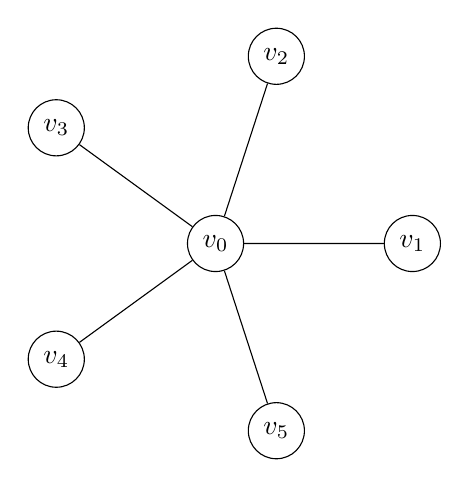
\begin{tikzpicture}[scale=2.5]
\tikzstyle{every node}=[draw,shape=circle];
\path (0:0cm)    node (v0) {$v_0$};
\path (0:1cm)    node (v1) {$v_1$};
\path (72:1cm)   node (v2) {$v_2$};
\path (2*72:1cm) node (v3) {$v_3$};
\path (3*72:1cm) node (v4) {$v_4$};
\path (4*72:1cm) node (v5) {$v_5$};
\draw (v0) -- (v1)
      (v0) -- (v2)
      (v0) -- (v3)
      (v0) -- (v4)
      (v0) -- (v5);
\end{tikzpicture}
\end{figure}
\end{filecontents*}

\subsection{tikz/pgf}
\IfElsePackageLoaded{graphicx}{%
\IfElsePackageLoaded{tikz}{%

\subsubsection{basic nodes}
\PrintDemo{style=stacked}%

}{\DemoError{Package \package{tikz} not loaded}}%
}{\DemoError{Package \package{graphicx} not loaded}}%


%% ------------------------------------------------------------
\begin{filecontents*}{\democodefile}
\begin{figure}[H]
\centering
% code origin: 
% http://www.texample.net/tikz/examples/rotated-polygons/
\newcounter{density}
\setcounter{density}{20}
\begin{tikzpicture}[scale=0.75]
  \def\couleur{OrangeRed}
  \path[coordinate] (0,0)  coordinate(A)
        ++( 90:12cm) coordinate(B)
        ++(  0:12cm) coordinate(C)
        ++(-90:12cm) coordinate(D);
  \draw[fill=\couleur!\thedensity] (A) -- (B) -- (C) --(D) -- cycle;
  \foreach \x in {1,...,40}{%
    \pgfmathsetcounter{density}{\thedensity+20}
    \setcounter{density}{\thedensity}
    \path[coordinate] coordinate(X) at (A){};
    \path[coordinate] (A) 
              -- (B) coordinate[pos=.10](A)
              -- (C) coordinate[pos=.10](B)
              -- (D) coordinate[pos=.10](C)
              -- (X) coordinate[pos=.10](D);
    \draw[fill=\couleur!\thedensity] (A)--(B)--(C)-- (D) -- cycle;
  }
\end{tikzpicture}
\end{figure}
\end{filecontents*}

\IfElsePackageLoaded{graphicx}{%
\IfElsePackageLoaded{tikz}{%
\IfColorDefined{OrangeRed}{

\subsubsection{for each example}
\PrintDemo{style=stacked}%

}{\DemoError{Package \package{xcolor} not loaded, Color \emph{OrangeRed} not defined}}%
}{\DemoError{Package \package{tikz} not loaded}}%
}{}%

%% ------------------------------------------------------------
\begin{filecontents*}{\democodefile}
\begin{figure}[H]
\centering
% code origin: pgf/tikz manual
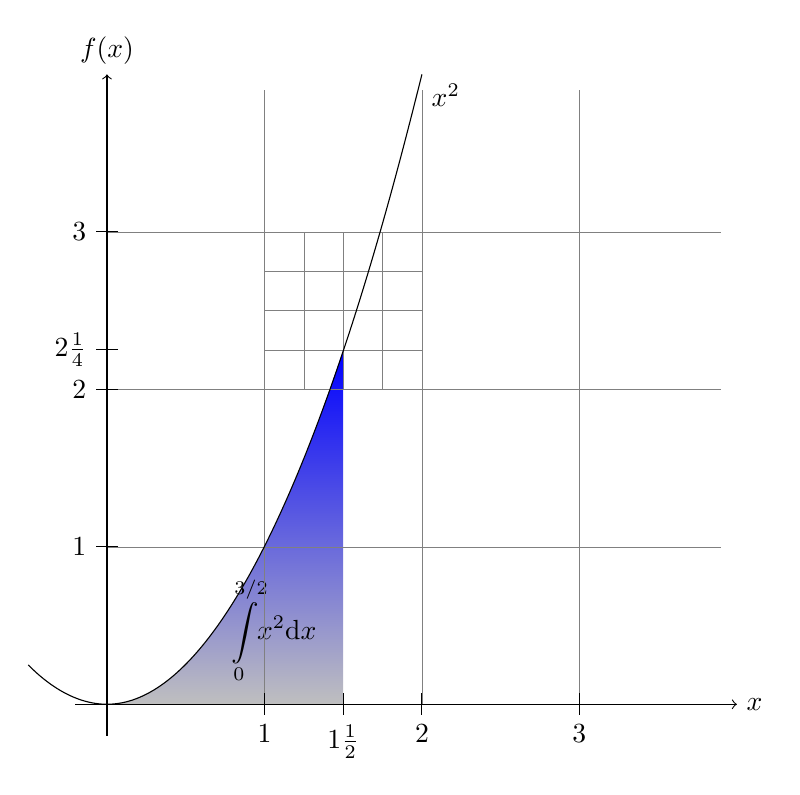
\begin{tikzpicture}[scale=2]
  \shade[top color=blue,bottom color=gray!50] 
    (0,0) parabola (1.5,2.25) |- (0,0);
  \draw (1.05cm,2pt) node[above] 
    {$\displaystyle\int_0^{3/2} \!\!x^2\mathrm{d}x$};
  \draw[help lines]  (0,0) grid (3.9,3.9)
       [step=0.25cm] (1,2) grid +(1,1);
  \draw[->] (-0.2,0) -- (4,0) node[right] {$x$};
  \draw[->] (0,-0.2) -- (0,4) node[above] {$f(x)$};
  \foreach \x/\xtext in {1/1, 1.5/1\frac{1}{2}, 2/2, 3/3}
    \draw[shift={(\x,0)}] (0pt,2pt) -- (0pt,-2pt) node[below] {$\xtext$};
  \foreach \y/\ytext in {1/1, 2/2, 2.25/2\frac{1}{4}, 3/3}
    \draw[shift={(0,\y)}] (2pt,0pt) -- (-2pt,0pt) node[left] {$\ytext$};
  \draw (-.5,.25) parabola bend (0,0) (2,4) node[below right] {$x^2$};
\end{tikzpicture}
\end{figure}
\end{filecontents*}

\IfElsePackageLoaded{graphicx}{%
\IfElsePackageLoaded{tikz}{%

\subsubsection{Fancy plot with tikz}
\PrintDemo{style=stacked}%

}{\DemoError{Package \package{tikz} not loaded}}%
}{}%

%% ------------------------------------------------------------
\begin{filecontents*}{\democodefile}
\begin{figure}[H]
\centering
% code origin: pgf/tikz manual
\begin{tikzpicture}[rotate=-90, scale = 0.9,
                    circuit ee IEC,
                    x=3.25cm,y=2.25cm,semithick,
                    every info/.style={font=\footnotesize},
                    small circuit symbols,
                    set resistor graphic=var resistor IEC graphic,
                    set diode graphic=var diode IEC graphic,
                    set make contact graphic= var make contact IEC graphic]
% Let us start with some contacts:
\foreach \contact/\y in {1/1,2/2,3/3.5,4/4.5,5/5.5}
{
      \node [contact] (left contact \contact) at (0,\y) {};
      \node [contact] (right contact \contact) at (1,\y) {};
}
\draw  (right contact 1) -- (right contact 2) -- (right contact 3)
    -- (right contact 4) -- (right contact 5);
%
\draw (left contact 1) to [diode] ++(down:1)
                       to [voltage source={near start,
                                           direction info={volt=3}},
                          resistor={near end,ohm=3}] ++(right:1)
                       to (right contact 1);
%
\draw (left contact 1) to [resistor={ohm=4}] (right contact 1);
\draw (left contact 1) to [resistor={ohm=3}] (left contact 2);
\draw (left contact 2) to [voltage source={near start,
                                           direction info={<-,volt=8}},
                           resistor={ohm=2,near end}] (right contact 2);
%
\draw (left contact 2) to [resistor={near start,ohm=1},
                           make contact={near end,info'={[red]$S_1$}}]
                           (left contact 3);
%
\draw (left contact 3) to [current direction'={near start,info=$\iota$},
                           resistor={near end,info={$R=4\Omega$}}]
                           (right contact 3);
%
\draw (left contact 4) to [voltage source={near start,
                           direction info={<-,volt=8}},
                           resistor={ohm=2,near end}] (right contact 4);
%
\draw (left contact 3) to [resistor={ohm=1}] (left contact 4);
\draw (left contact 4) to [resistor={ohm=3}] (left contact 5);
\draw (left contact 5) to [resistor={ohm=4}] (right contact 5);
\draw (left contact 5) to [diode] ++(up:1)
                       to [voltage source={near start,
                           direction info={volt=3}},
                           resistor={near end,ohm=3}] ++(right:1)
                       to (right contact 5);
\end{tikzpicture}
\end{figure}
\end{filecontents*}

\IfElsePackageLoaded{graphicx}{%
\IfElsePackageLoaded{tikz}{%

\subsubsection{Circuit Libraries}

\IfTikzLibraryLoaded{circuits}{
\PrintDemo{style=stacked}%
}{\DemoError{tikz library `circuits' not loaded}}
}{\DemoError{Package \package{tikz} not loaded}}%
}{}%

%% ------------------------------------------------------------
\begin{filecontents*}{\democodefile}
\begin{figure}[H]
\centering
% code origin: pgf/tikz manual
\begin{tikzpicture}
\pgfdeclarelindenmayersystem{Koch curve}{
   \rule{F -> F-F++F-F}
}
\shadedraw [top color=white, bottom color=blue!50, draw=blue!50!black]
           [l-system={Koch curve, step=2pt, angle=60, axiom=F++F++F, order=3}]
           lindenmayer system -- cycle;
\end{tikzpicture}
\end{figure}
\end{filecontents*}

\IfElsePackageLoaded{graphicx}{%
\IfElsePackageLoaded{tikz}{%

\subsubsection{Lindenmayer System Drawing Library}

\IfTikzLibraryLoaded{lindenmayersystems}{

\PrintDemo{style=stacked}%

}{\DemoError{tikz library `lindenmayer' not loaded}}
}{\DemoError{Package \package{tikz} not loaded}}%
}{}%

%% ------------------------------------------------------------
\begin{filecontents*}{\democodefile}
\begin{figure}[H]
\centering
% code origin: pgf/tikz manual
\begin{tikzpicture}
  \path[mindmap,concept color=black,text=white]
    node[concept] {Computer Science}
    [clockwise from=0]
    % note that `sibling angle' can only be defined in
    % `level 1 concept/.append style={}'
    child[concept color=green!50!black] {
      node[concept] {practical}
      [clockwise from=90]
      child { node[concept] {algorithms} }
      child { node[concept] {data structures} }
      child { node[concept] {pro\-gramming languages} }
      child { node[concept] {software engineer\-ing} }
    }
    child[concept color=blue] {
      node[concept] {applied}
      [clockwise from=-30]
      child { node[concept] {databases} }
      child { node[concept] {WWW} }
    }
    child[concept color=red] { node[concept] {technical} }
    child[concept color=orange] { node[concept] {theoretical} };
\end{tikzpicture}
\end{figure}
\end{filecontents*}

\IfElsePackageLoaded{graphicx}{%
\IfElsePackageLoaded{tikz}{%

\subsubsection{Mindmap Drawing Library}

\IfTikzLibraryLoaded{mindmap}{
\PrintDemo{style=stacked}%
}{\DemoError{tikz library `mindmap' not loaded}}
}{\DemoError{Package \package{tikz} not loaded}}%
}{}%

%% ------------------------------------------------------------
\begin{filecontents*}{\democodefile}
\begin{figure}[H]
\centering
% code origin: pgf/tikz manual
\begin{tikzpicture}[scale=2]
\shade[upper left=red,upper right=green,
      lower left=blue,lower right=yellow]       
  (0,0) rectangle (3,2);
\end{tikzpicture}
\end{figure}
\end{filecontents*}

\IfElsePackageLoaded{graphicx}{%
\IfElsePackageLoaded{tikz}{%

\subsubsection{Shadings Library}

\IfTikzLibraryLoaded{shadings}{
\PrintDemo{style=stacked}%

}{\DemoError{tikz library `shadings' not loaded}}
}{\DemoError{Package \package{tikz} not loaded}}%
}{}%
%
%% ------------------------------------------------------------
\begin{filecontents*}{\democodefile}
\begin{figure}[H]
\centering
% code origin: pgf/tikz manual
\begin{tikzpicture}[shorten >=1pt,node distance=2cm,on grid]
  \node[state,initial] (q_0) {$q_0$};
  \node[state] (q_1) [right=of q_0] {$q_1$};
  \node[state,accepting](q_2) [right=of q_1] {$q_2$};
  \path[->] (q_0) edge node [above] {0} (q_1)
                  edge [loop above] node {1} ()
                  edge [bend left] node [above] {1} (q_2)
                  edge [bend right] node [below] {0} (q_2)
            (q_1) edge node [above] {1} (q_2);
\end{tikzpicture}
\end{figure}
\end{filecontents*}

\IfElsePackageLoaded{graphicx}{%
\IfElsePackageLoaded{tikz}{%

\subsubsection{Automata Drawing and To Path Library}

\IfTikzLibraryLoaded{automata}{
\IfTikzLibraryLoaded{topaths}{
\PrintDemo{style=stacked}%

}{\DemoError{tikz library `topaths' not loaded}}%
}{\DemoError{tikz library `automata' not loaded}}%
}{\DemoError{Package \package{tikz} not loaded}}%
}{}%

%% ------------------------------------------------------------
\clearpage
\subsection{pgfplots}
%% ------------------------------------------------------------
\begin{filecontents*}{\democodefile}
\begin{figure}[H]
\pgfplotsset{width=0.8\textwidth, height=0.6\textwidth}
\centering
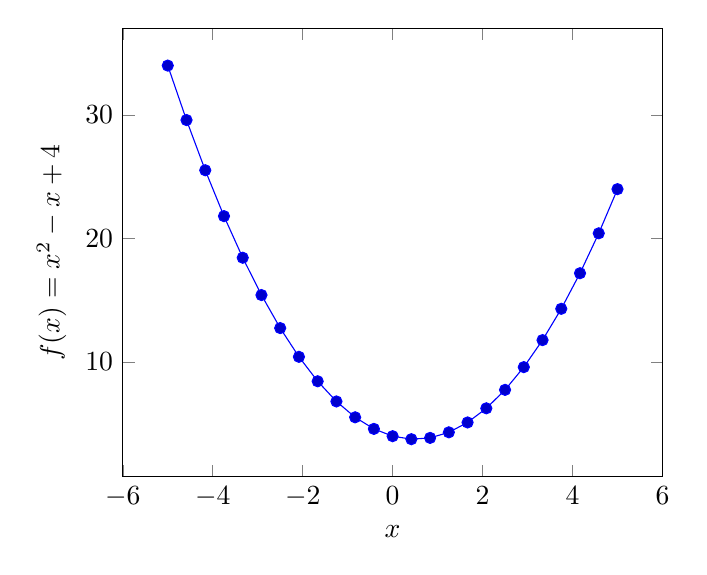
\begin{tikzpicture}
\begin{axis}[
  xlabel=$x$,
  ylabel={$f(x) = x^2 - x +4$}
]
% use TeX as calculator:
\addplot {x^2 - x +4};
\end{axis}
\end{tikzpicture}
\end{figure}
\end{filecontents*}

\IfElsePackageLoaded{graphicx}{%
\IfElsePackageLoaded{pgfplots}{%

\subsubsection{Simple plot with curve (calculated by TeX)}
\PrintDemo{style=stacked}%

}{\DemoError{Package \package{pgfplots} not loaded}}%
}{\DemoError{Package \package{graphicx} not loaded}}%


%% ------------------------------------------------------------
\begin{filecontents*}{\democodefile}
\begin{figure}[H]
\pgfplotsset{width=0.8\textwidth, height=0.6\textwidth}
\pgfplotsset{samples=2000}
\centering
\begin{tikzpicture}
\begin{axis}[
  xlabel=$x$,
  ylabel={$\sin(x) (x+1) + 3x$},
  grid=major,
  /pgfplots/enlargelimits=false,
  ymax=500,
  /pgfplots/xtick={0,20,...,100},
  /pgfplots/ytick={0,100,...,600},
]
%
\addplot[domain=0:100, blue,style={line width=0.7pt}]
  gnuplot{sin(x)*(x+1) + 3*x};
%
\legend{$\sin(x) (x+1) + 3x$}
\end{axis}
\end{tikzpicture}
\end{figure}
\end{filecontents*}

\IfElsePackageLoaded{graphicx}{%
\IfElsePackageLoaded{pgfplots}{%

\subsubsection{Simple plot with curve (calculated by gnuplot)}
\PrintDemo{style=stacked}%

}{\DemoError{Package \package{pgfplots} not loaded}}%
}{}%

%% ------------------------------------------------------------
\begin{filecontents*}{\democodefile}
\begin{figure}[H]
\pgfplotsset{width=0.8\textwidth, height=0.6\textwidth}
\centering
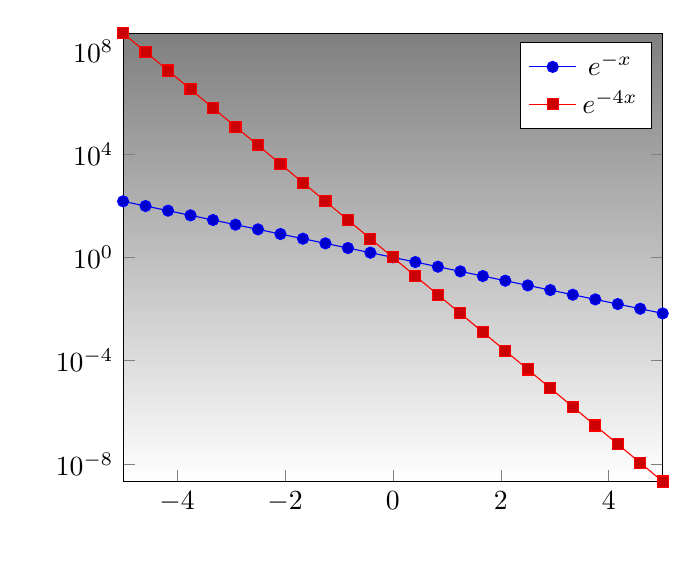
\begin{tikzpicture}
  \begin{semilogyaxis}[
    axis background/.style={shade,top color=gray,bottom color=white},
    legend style={fill=white},
    /pgfplots/enlargelimits=false]
    %
    \addplot {exp(-x)};
    \addplot {exp(-4*x)};
    %
    \legend{$e^{-x}$,$e^{-4x}$}
  \end{semilogyaxis}
\end{tikzpicture}
\end{figure}
\end{filecontents*}

\IfElsePackageLoaded{graphicx}{%
\IfElsePackageLoaded{pgfplots}{%

\subsubsection{Semilog axis with filled background}
\PrintDemo{style=stacked}%

}{\DemoError{Package \package{pgfplots} not loaded}}%
}{}%


%% ------------------------------------------------------------
\begin{filecontents*}{\democodefile}
\begin{figure}[H]
\pgfplotsset{width=0.8\textwidth, height=0.6\textwidth}
\centering
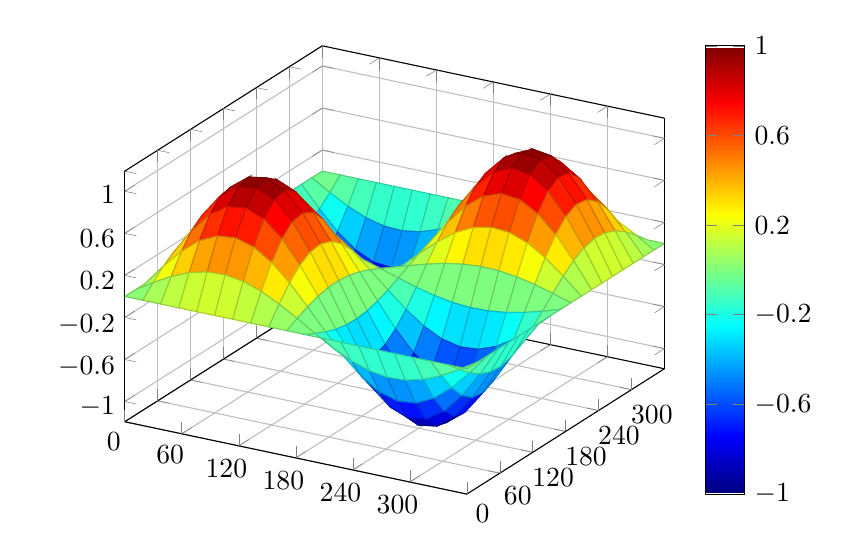
\begin{tikzpicture}
\begin{axis}[view={30}{30},grid=major,
   /pgfplots/xtick={0,60,...,300},
   /pgfplots/ytick={0,60,...,300},
   /pgfplots/ztick={-1.0,-0.6,...,1.0},
   colorbar,
   colorbar style={ytick={-1.0,-0.6,...,1.0},
                   ymin=-1,ymax=1},
   colormap/jet
]
\addplot3[surf,domain=0:360,samples=20]
  {sin(x)*sin(y)};
\end{axis}
\end{tikzpicture}
\end{figure}
\end{filecontents*}

\IfElsePackageLoaded{graphicx}{%
\IfElsePackageLoaded{pgfplots}{%

\subsubsection{3D plot}
\PrintDemo{style=stacked}%

}{\DemoError{Package \package{pgfplots} not loaded}}%
}{}%


%% ------------------------------------------------------------
\begin{filecontents*}{plotdata.txt}
0	0
0.15787	0.18867
0.31574	0.37913
0.47361	0.56789
0.63148	0.75108
0.78934	0.92486
0.94721	1.0858
1.1051	1.2316
1.263	1.361
1.4208	1.4748
1.5787	1.5756
1.7366	1.6678
1.8944	1.7577
2.0523	1.8526
2.2102	1.9604
2.368	2.0888
2.5259	2.244
2.6838	2.4303
2.8416	2.6488
2.9995	2.8973
3.1574	3.1697
3.3152	3.4564
3.4731	3.745
3.631	4.021
3.7889	4.2697
3.9467	4.4773
4.1046	4.6331
4.2625	4.7308
4.4203	4.7698
4.5782	4.7562
4.7361	4.7024
4.8939	4.6272
5.0518	4.5536
5.2097	4.5074
5.3675	4.5139
5.5254	4.5958
5.6833	4.7695
5.8412	5.0433
5.999	5.4152
6.1569	5.8721
6.3148	6.3902
6.4726	6.9367
6.6305	7.472
6.7884	7.9544
6.9462	8.3437
7.1041	8.6062
7.262	8.7188
7.4198	8.6729
7.5777	8.4764
7.7356	8.1542
7.8934	7.7469
8.0513	7.3081
8.2092	6.8988
8.3671	6.5819
8.5249	6.4152
8.6828	6.4448
8.8407	6.699
8.9985	7.1839
9.1564	7.8815
9.3143	8.7493
9.4721	9.7239
9.63	10.726
9.7879	11.669
9.9457	12.466
10.104	13.041
10.261	13.336
10.419	13.323
10.577	13
10.735	12.402
10.893	11.593
11.051	10.663
11.209	9.7198
11.367	8.8774
11.524	8.2443
11.682	7.9121
11.84	7.9444
11.998	8.369
12.156	9.1739
12.314	10.306
12.472	11.677
12.63	13.17
12.787	14.65
12.945	15.982
13.103	17.04
13.261	17.724
13.419	17.97
13.577	17.76
13.735	17.119
13.892	16.121
14.05	14.877
14.208	13.526
14.366	12.22
14.524	11.109
14.682	10.325
14.84	9.9681
14.998	10.094
15.155	10.71
15.313	11.773
15.471	13.193
15.629	14.843
15.787	16.573
15.945	18.223
16.103	19.643
16.261	20.706
16.418	21.322
16.576	21.448
16.734	21.091
16.892	20.307
17.05	19.196
17.208	17.89
17.366	16.539
17.523	15.295
17.681	14.297
17.839	13.656
17.997	13.446
18.155	13.692
18.313	14.376
18.471	15.434
18.629	16.766
18.786	18.246
18.944	19.739
19.102	21.11
19.26	22.242
19.418	23.047
19.576	23.472
19.734	23.504
19.891	23.172
20.049	22.539
20.207	21.696
20.365	20.753
20.523	19.823
20.681	19.014
20.839	18.416
20.997	18.093
21.154	18.08
21.312	18.375
21.47	18.95
21.628	19.747
21.786	20.69
21.944	21.692
22.102	22.667
22.26	23.534
22.417	24.232
22.575	24.717
22.733	24.971
22.891	25.001
23.049	24.834
23.207	24.517
23.365	24.108
23.522	23.669
23.68	23.262
23.838	22.94
23.996	22.743
24.154	22.697
24.312	22.81
24.47	23.072
24.628	23.461
24.785	23.944
24.943	24.479
25.101	25.026
25.259	25.544
25.417	26.001
25.575	26.373
25.733	26.646
25.891	26.82
26.048	26.902
26.206	26.909
26.364	26.862
26.522	26.789
26.68	26.713
26.838	26.66
26.996	26.646
27.153	26.685
27.311	26.783
27.469	26.939
27.627	27.146
27.785	27.395
27.943	27.671
28.101	27.96
28.259	28.246
28.416	28.519
28.574	28.767
28.732	28.986
28.89	29.172
29.048	29.327
29.206	29.455
29.364	29.563
29.521	29.658
29.679	29.748
29.837	29.84
29.995	29.941
30.153	30.055
30.311	30.184
30.469	30.33
30.627	30.491
30.784	30.665
30.942	30.848
31.1	31.037
31.258	31.227
31.416	31.416
\end{filecontents*}

\begin{filecontents*}{\democodefile}
\begin{figure}[H]
\pgfplotsset{width=0.8\textwidth, height=0.6\textwidth}
\centering
\begin{tikzpicture}
\begin{axis}[scale only axis,/pgfplots/enlargelimits=false]
  \addplot[style=solid, color=blue, mark=none,
           style={line width=0.7pt}]
    file{plotdata.txt};
\end{axis}
\end{tikzpicture}
\end{figure}
\end{filecontents*}

\IfElsePackageLoaded{graphicx}{%
\IfElsePackageLoaded{pgfplots}{%

\subsubsection{Plotting data from a file}
\PrintDemo{style=stacked}%

}{\DemoError{Package \package{pgfplots} not loaded}}%
}{}%

%% ------------------------------------------------------------
\begin{filecontents*}{\democodefile}
\begin{figure}[H]
\pgfplotsset{width=0.8\textwidth, height=0.6\textwidth}
\centering
\begin{tikzpicture}
\begin{axis}[scale only axis,
             /pgfplots/enlargelimits=false,
             ymax = 34,
             legend cell align=left,
             legend style={
               cells={anchor=west},
               legend pos=north west,
               font=\small
             }]
  \addplot[style=solid, color=blue, mark=none, style={line width=0.7pt}]
    file {plotdata.txt};
    %
  \addplot [raw gnuplot,
            style=solid, color=red, mark=none, style={line width=0.7pt}]
    gnuplot [id=plotdata] {
      % define function which should be fitted
      f(x)=a*x;
      % let gnuplot fit using column 1 and 2 of the data file
      fit f(x) 'plotdata.txt' using 1:2 via a;
      % Plot the function with the specified plot range
      plot [x=0:30] f(x); 
    };  
  %
  \legend{{\raisebox{2.5ex}{
          $f(x) = 5\exp\left(-\left(\dfrac{x-5\pi}{2.5\pi}\right)^2\right)
                   \sin(2x) + x$}},
          $f(x)_\text{fit} = x$}
\end{axis}
\end{tikzpicture}
\end{figure}
\end{filecontents*}

\IfElsePackageLoaded{graphicx}{%
\IfElsePackageLoaded{pgfplots}{%

\subsubsection{fitting with gnuplot}
\PrintDemo{style=stacked}%

}{\DemoError{Package \package{pgfplots} not loaded}}%
}{}%


%% ------------------------------------------------------------
\subsubsection{plotting multiple lines from single file}
\begin{filecontents*}{plotdata.txt}
x1	y1	y2	y3	y4
0	0.05754	4.858e-016	4.5469e-063	2.4067e-174
0.31733	0.085313	2.9249e-015	5.5675e-061	5.5022e-170
0.63467	0.12393	1.682e-014	6.2829e-059	1.1073e-165
0.952	0.1764	9.2386e-014	6.5344e-057	1.9616e-161
1.2693	0.24602	4.8467e-013	6.2633e-055	3.0588e-157
1.5867	0.33617	2.4285e-012	5.5329e-053	4.1987e-153
1.904	0.45008	1.1622e-011	4.5046e-051	5.0733e-149
2.2213	0.59041	5.3126e-011	3.3799e-049	5.396e-145
2.5387	0.75886	2.3195e-010	2.3373e-047	5.0521e-141
2.856	0.95566	9.6721e-010	1.4896e-045	4.1637e-137
3.1733	1.1792	3.8523e-009	8.7492e-044	3.0206e-133
3.4907	1.4256	1.4655e-008	4.7361e-042	1.929e-129
3.808	1.6887	5.3246e-008	2.3628e-040	1.0843e-125
4.1253	1.96	1.8478e-007	1.0864e-038	5.3655e-122
4.4427	2.2289	6.1249e-007	4.6036e-037	2.3371e-118
4.76	2.4835	1.9391e-006	1.7979e-035	8.9607e-115
5.0773	2.7112	5.8634e-006	6.4709e-034	3.0243e-111
5.3947	2.9001	1.6934e-005	2.1465e-032	8.985e-108
5.712	3.0394	4.6713e-005	6.5621e-031	2.3498e-104
6.0293	3.1211	0.00012308	1.8489e-029	5.4093e-101
6.3467	3.1403	0.00030972	4.8009e-028	1.0961e-097
6.664	3.0958	0.00074444	1.1489e-026	1.9553e-094
6.9813	2.9902	0.001709	2.534e-025	3.0701e-091
7.2986	2.8299	0.0037473	5.1508e-024	4.2434e-088
7.616	2.6241	0.0078479	9.6492e-023	5.1627e-085
7.9333	2.3841	0.015698	1.6659e-021	5.5292e-082
8.2506	2.1224	0.029992	2.6508e-020	5.2126e-079
8.568	1.8511	0.054729	3.8873e-019	4.3257e-076
8.8853	1.582	0.095387	5.2538e-018	3.1599e-073
9.2026	1.3246	0.15879	6.5441e-017	2.0319e-070
9.52	1.0868	0.25248	7.5123e-016	1.1501e-067
9.8373	0.87359	0.38342	7.9479e-015	5.7303e-065
10.155	0.68805	0.55615	7.7496e-014	2.5133e-062
10.472	0.53097	0.77048	6.9639e-013	9.703e-060
10.789	0.40147	1.0195	5.7674e-012	3.2975e-057
11.107	0.29743	1.2885	4.4021e-011	9.8645e-055
11.424	0.2159	1.5554	3.0967e-010	2.5976e-052
11.741	0.15355	1.7933	2.0076e-009	6.0213e-050
12.059	0.107	1.9749	1.1995e-008	1.2286e-047
12.376	0.073057	2.0772	6.6053e-008	2.2067e-045
12.693	0.048874	2.0867	3.3522e-007	3.4889e-043
13.011	0.032035	2.0022	1.5679e-006	4.8557e-041
13.328	0.020574	1.835	6.7585e-006	5.9486e-039
13.645	0.012946	1.6062	2.685e-005	6.415e-037
13.963	0.0079819	1.3429	9.8306e-005	6.0895e-035
14.28	0.0048218	1.0723	0.00033172	5.0884e-033
14.597	0.002854	0.81787	0.0010316	3.7428e-031
14.915	0.0016551	0.5958	0.0029567	2.4234e-029
15.232	0.00094047	0.41455	0.0078099	1.3812e-027
15.549	0.0005236	0.27549	0.019012	6.9294e-026
15.867	0.00028562	0.17486	0.042656	3.0602e-024
16.184	0.00015266	0.10601	0.088202	1.1896e-022
16.501	7.9943e-005	0.061386	0.16808	4.0709e-021
16.819	4.1019e-005	0.03395	0.29521	1.2263e-019
17.136	2.0622e-005	0.017934	0.47783	3.2515e-018
17.453	1.0158e-005	0.0090483	0.71281	7.5891e-017
17.771	4.9026e-006	0.0043603	0.98	1.5592e-015
18.088	2.3184e-006	0.0020069	1.2417	2.8199e-014
18.405	1.0742e-006	0.00088228	1.45	4.4893e-013
18.723	4.8765e-007	0.00037046	1.5606	6.2912e-012
19.04	2.1691e-007	0.00014857	1.5479	7.7607e-011
19.357	9.4533e-008	5.6909e-005	1.415	8.427e-010
19.675	4.0367e-008	2.0821e-005	1.1921	8.0549e-009
19.992	1.6889e-008	7.2756e-006	0.92557	6.7773e-008
20.309	6.9235e-009	2.4283e-006	0.66232	5.0196e-007
20.627	2.7809e-009	7.741e-007	0.4368	3.2725e-006
20.944	1.0944e-009	2.3569e-007	0.26549	1.8781e-005
21.261	4.22e-010	6.8542e-008	0.14871	9.4876e-005
21.579	1.5944e-010	1.9038e-008	0.076774	0.0004219
21.896	5.9019e-011	5.0508e-009	0.036528	0.0016515
22.213	2.1406e-011	1.2798e-009	0.016018	0.0056904
22.531	7.6072e-012	3.0975e-010	0.0064731	0.01726
22.848	2.6488e-012	7.1601e-011	0.0024109	0.046081
23.165	9.0366e-013	1.5809e-011	0.00082756	0.1083
23.483	3.0207e-013	3.3337e-012	0.0002618	0.22405
23.8	9.8932e-014	6.7145e-013	7.6328e-005	0.40802
24.117	3.1748e-014	1.2917e-013	2.051e-005	0.65406
24.435	9.9821e-015	2.3735e-014	5.079e-006	0.92293
24.752	3.0752e-015	4.1654e-015	1.1592e-006	1.1464
25.069	9.2823e-016	6.9821e-016	2.4382e-007	1.2534
25.387	2.7452e-016	1.1178e-016	4.7266e-008	1.2064
25.704	7.955e-017	1.7093e-017	8.4446e-009	1.0221
26.021	2.2586e-017	2.4965e-018	1.3905e-009	0.76223
26.339	6.2831e-018	3.4827e-019	2.11e-010	0.50038
26.656	1.7126e-018	4.6403e-020	2.951e-011	0.28915
26.973	4.5737e-019	5.9052e-021	3.8036e-012	0.14708
27.291	1.1968e-019	7.1777e-022	4.5183e-013	0.065859
27.608	3.0683e-020	8.3329e-023	4.9466e-014	0.025958
27.925	7.7078e-021	9.2399e-024	4.991e-015	0.0090063
28.243	1.8971e-021	9.7858e-025	4.6411e-016	0.0027506
28.56	4.575e-022	9.8989e-026	3.9775e-017	0.00073947
28.877	1.081e-022	9.564e-027	3.1416e-018	0.00017499
29.195	2.5027e-023	8.8257e-028	2.2868e-019	3.6453e-005
29.512	5.6771e-024	7.779e-029	1.5342e-020	6.6844e-006
29.829	1.2618e-024	6.5487e-030	9.4855e-022	1.0789e-006
30.147	2.7477e-025	5.2655e-031	5.4051e-023	1.533e-007
30.464	5.8626e-026	4.0438e-032	2.8385e-024	1.9174e-008
30.781	1.2256e-026	2.9662e-033	1.3738e-025	2.1109e-009
31.099	2.5105e-027	2.0781e-034	6.1281e-027	2.0458e-010
31.416	5.0385e-028	1.3906e-035	2.5193e-028	1.7452e-011
\end{filecontents*}

\begin{filecontents*}{\democodefile}
\begin{figure}[H]
\centering
\pgfplotsset{width=0.8\textwidth, height=0.6\textwidth}
% read data to table
\pgfplotstableread{plotdata.txt}\datatable
%
\begin{tikzpicture}
\begin{axis}[scale only axis,
             every axis plot/.append style={line width=1.5pt},
             mark=none, style=solid,
             enlargelimits=false, ymax = 3.5,
             cycle list name=colorseries-office,
             smooth]
  %  column with header  "y1", "y2", ...
  \addplot+ table[x=x1,y=y1]  from  \datatable;
  \addplot+ table[x=x1,y=y2]  from  \datatable;
  \addplot+ table[x=x1,y=y3]  from  \datatable;
  \addplot+ table[x=x1,y=y4]  from  \datatable;
\end{axis}
\end{tikzpicture}
\end{figure}
\end{filecontents*}

\IfElsePackageLoaded{graphicx}{%
\IfElsePackageLoaded{pgfplots}{%

\PrintDemo{style=stacked}%

}{\DemoError{Package \package{pgfplots} not loaded}}%
}{}%




\EndCodeSection{DemoDiagrams}

% -- bibliography --
% (must be placed _before_ appendix)
\IfPackageLoaded{biblatex}{
  \printbibliography[%
    heading=bibintoc, % (bibintoc, bibnumbered)
  ]	
}

%% -- list of figures and tables --
\clearpage
\listoffigures
\listoftables
\cleardoublepage
\IfDefined{lstlistoflistings}{\lstlistoflistings}
\cleardoublepage
\IfDefined{printindex}{\printindex}

\typeout{time elapsed: \the\pdfelapsedtime/65536 s}

%%% Dokument END %%%%%%%%%%%%%%%%%%%%%%%%%%%%%%%%%%%%%%%%%%%%%%%%%%%%%%%%%%%
\end{document}
%%%%%%%%%%%%%%%%%%%%%%%%%%%%%%%%%%%%%%%%%%%%%%%%%%%%%%%%%%%%%%%%%%%%%%%%%%%%
